\documentclass[11pt,a4paper]{article}

\usepackage[T1]{fontenc}
\usepackage[utf8]{inputenc}
\usepackage{lmodern}
\usepackage[margin=2.2cm]{geometry}
\usepackage{amsmath,amssymb,amsthm,mathtools}
\usepackage{bm}
\usepackage{booktabs}
\usepackage{array}
\usepackage{xcolor}
\usepackage{graphicx}
\usepackage{tikz}
\usetikzlibrary{arrows.meta,calc,positioning,shapes.geometric}
\usepackage{enumitem}
\usepackage[colorlinks=true,linkcolor=blue!60!black,citecolor=blue!60!black,urlcolor=blue!60!black]{hyperref}

\setlength{\emergencystretch}{3em}
\setlength{\parskip}{4pt}

\definecolor{atomblue}{RGB}{41,128,185}
\definecolor{defectred}{RGB}{211,47,47}
\definecolor{okgreen}{RGB}{46,125,50}
\definecolor{amberh}{RGB}{245,158,11}
\definecolor{boxbg}{RGB}{245,248,252}
\definecolor{boxframe}{RGB}{180,200,225}
\definecolor{warnbg}{RGB}{255,248,235}
\definecolor{warnframe}{RGB}{225,180,100}

\newcommand{\R}{\mathbb{R}}
\newcommand{\Z}{\mathbb{Z}}
\newcommand{\T}{^{\mathsf T}}
\newcommand{\mT}{^{-\mathsf T}}
\newcommand{\tr}{\operatorname{tr}}
\newcommand{\Cred}{\mathbf{C}_{\mathrm{red}}}
\newcommand{\code}[1]{\texttt{#1}}

\newtheorem{proposition}{Proposition}

\newenvironment{keyidea}[1][Key Physical Idea]{%
  \par\medskip\noindent
  \begin{tikzpicture}
    \node[draw=boxframe,fill=boxbg,rounded corners=4pt,inner sep=10pt,text width=\dimexpr\textwidth-22pt\relax] (box) \bgroup
    \textbf{\textcolor{blue!60!black}{#1.}}\par\smallskip
}{%
    \egroup;
  \end{tikzpicture}\par\medskip
}

\newenvironment{cautionbox}[1][Numerical Subtlety]{%
  \par\medskip\noindent
  \begin{tikzpicture}
    \node[draw=warnframe,fill=warnbg,rounded corners=4pt,inner sep=10pt,text width=\dimexpr\textwidth-22pt\relax] (box) \bgroup
    \textbf{\textcolor{orange!75!black}{#1.}}\par\smallskip
}{%
    \egroup;
  \end{tikzpicture}\par\medskip
}

\title{\textbf{Coupling Dislocation Plasticity and Hydrogen Diffusion in the Mesoscopic Tensorial Model (MTM)}\\[6pt]
\large Variational Formulation, FEM Discretization Order, Delaunay Remeshing Invariance, and Staggered Solution Algorithms}
\author{MTM Lattice-Triangulation Technical Reference}
\date{November 2026}

\begin{document}
\maketitle

\begin{abstract}
\noindent
Hydrogen embrittlement in crystalline metals arises from the multiscale interplay of discrete dislocation cores, grain-boundary disconnections, stress-driven interstitial diffusion, deep microstructural trapping, and bond decohesion. Neither molecular dynamics (restricted to nanosecond timescales where dislocations outrun diffusion) nor continuum crystal plasticity (which smears out discrete dislocation stress singularities and avalanche statistics) can resolve all of these ingredients simultaneously. This document formulates a thermodynamically consistent chemo-mechanical extension of the 2D Mesoscopic Tensorial Model (MTM) that couples $\mathrm{GL}(2,\Z)$-invariant finite-strain crystal plasticity and adaptive CGAL Delaunay remeshing with stress-assisted hydrogen transport and Oriani/McNabb--Foster trapping. We explain in detail: (i) how FEM dislocation energy minimization (preconditioned L-BFGS + Delaunay surgery) couples variationally to the hydrogen chemical potential and modifies the tangent Hessian soft modes; (ii) \emph{at which spatial FEM order} the hydrogen equations must be discretized ($P_1$ nodal / Voronoi control-volume FEM with $L^2$-projected hydrostatic stress and Scharfetter--Gummel edge stabilization) to overcome the $P_0$ stress-gradient paradox without breaking MTM's discrete lattice topology; (iii) why storing hydrogen per host atom at mesh nodes guarantees exact machine-precision mass conservation across arbitrary Delaunay edge-flip avalanches; and (iv) \emph{at which temporal and operator-splitting order} (L-stable BDF1 across avalanches, 2nd-order TR-BDF2 on elastic branches, quadratic Newton--CHOLMOD inner solves) the coupled equations should be integrated.
\end{abstract}

\tableofcontents
\newpage

% ============================================================================
\section{Visual Guide: Where Hydrogen Sits \& How \texorpdfstring{\code{EnergyFunctions.h}}{EnergyFunctions.h} Feels It}
\label{sec:visual_guide}
% ============================================================================

Before presenting the full thermodynamic and finite-element derivations, this section explains the entire coupling in two concrete pictures: \textbf{(1) where hydrogen physically and computationally lives on your MTM lattice}, and \textbf{(2) why passing local hydrogen parameters into your existing \code{EnergyFunctions.h} generates exact swelling forces and L-BFGS relaxation with zero changes to your force-assembly formulas.}

\subsection{Where Hydrogen Sits on the Mesh (\code{Point2D} vs.\ \code{ElementTriangle2D})}

\begin{figure}[ht!]
\centering
\resizebox{\textwidth}{!}{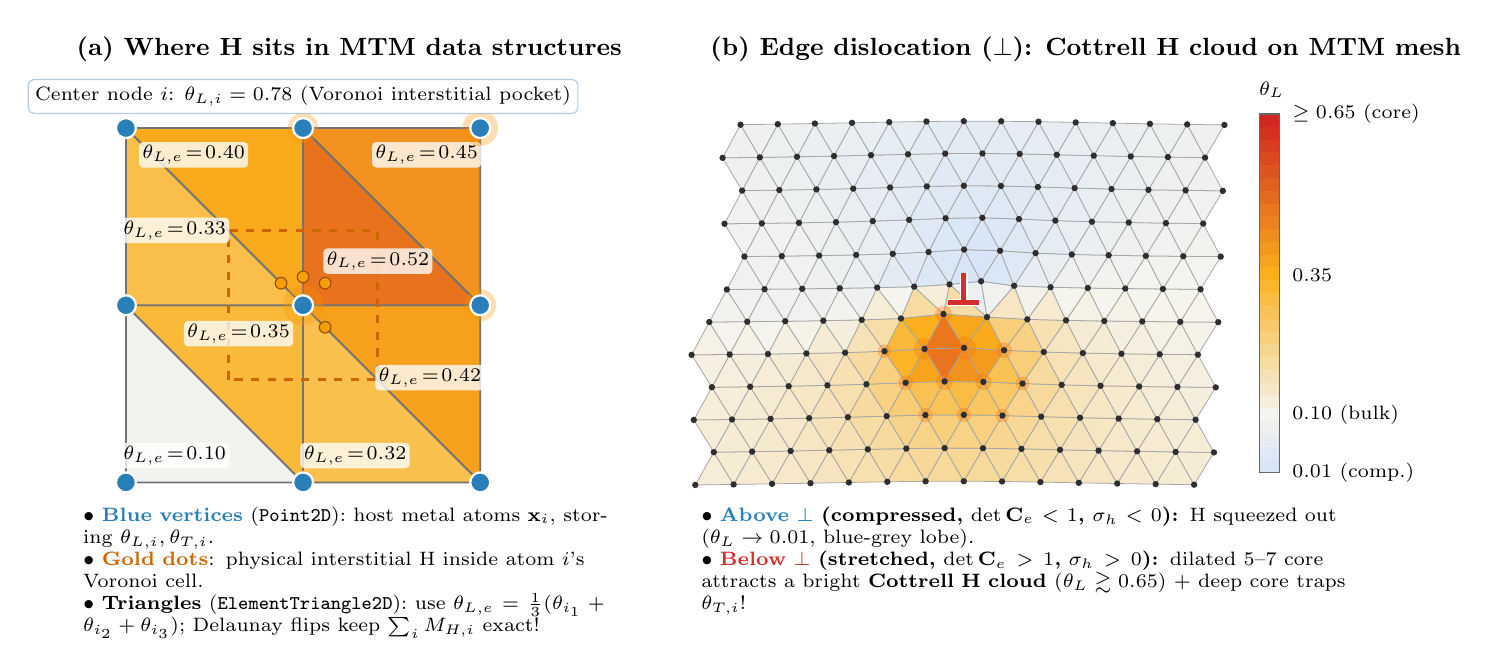
\begin{tikzpicture}[>=Stealth, font=\small]
  \node[anchor=west, font=\bfseries\small] at (0.0, 6.95) {(a) Where H sits in MTM data structures};
  \filldraw[fill={rgb,255:red,242;green,243;blue,239}, draw=black!55, line width=0.65pt] (0.750,1.450) -- (3.000,1.450) -- (0.750,3.700) -- cycle;
  \filldraw[fill={rgb,255:red,250;green,186;blue,57}, draw=black!55, line width=0.65pt] (3.000,3.700) -- (0.750,3.700) -- (3.000,1.450) -- cycle;
  \filldraw[fill={rgb,255:red,250;green,192;blue,78}, draw=black!55, line width=0.65pt] (3.000,1.450) -- (5.250,1.450) -- (3.000,3.700) -- cycle;
  \filldraw[fill={rgb,255:red,246;green,160;blue,28}, draw=black!55, line width=0.65pt] (5.250,3.700) -- (3.000,3.700) -- (5.250,1.450) -- cycle;
  \filldraw[fill={rgb,255:red,250;green,191;blue,73}, draw=black!55, line width=0.65pt] (0.750,3.700) -- (3.000,3.700) -- (0.750,5.950) -- cycle;
  \filldraw[fill={rgb,255:red,249;green,169;blue,28}, draw=black!55, line width=0.65pt] (3.000,5.950) -- (0.750,5.950) -- (3.000,3.700) -- cycle;
  \filldraw[fill={rgb,255:red,233;green,114;blue,30}, draw=black!55, line width=0.65pt] (3.000,3.700) -- (5.250,3.700) -- (3.000,5.950) -- cycle;
  \filldraw[fill={rgb,255:red,242;green,145;blue,29}, draw=black!55, line width=0.65pt] (5.250,5.950) -- (3.000,5.950) -- (5.250,3.700) -- cycle;
  \draw[dashed, orange!80!black, line width=1.1pt] (2.055,2.755) rectangle (3.945,4.645);
  \filldraw[fill=amberh, draw=orange!60!black, line width=0.4pt] (2.720,3.980) circle (2.1pt);
  \filldraw[fill=amberh, draw=orange!60!black, line width=0.4pt] (3.280,3.980) circle (2.1pt);
  \filldraw[fill=amberh, draw=orange!60!black, line width=0.4pt] (2.720,3.420) circle (2.1pt);
  \filldraw[fill=amberh, draw=orange!60!black, line width=0.4pt] (3.280,3.420) circle (2.1pt);
  \filldraw[fill=amberh, draw=orange!60!black, line width=0.4pt] (3.000,4.060) circle (2.1pt);
  \node[fill=white, fill opacity=0.78, text opacity=1, rounded corners=1.5pt, inner sep=1.2pt, font=\scriptsize] at (1.370,1.790) {$\theta_{L,e}\!=\!0.10$};
  \node[fill=white, fill opacity=0.78, text opacity=1, rounded corners=1.5pt, inner sep=1.2pt, font=\scriptsize] at (2.180,3.340) {$\theta_{L,e}\!=\!0.35$};
  \node[fill=white, fill opacity=0.78, text opacity=1, rounded corners=1.5pt, inner sep=1.2pt, font=\scriptsize] at (3.660,1.790) {$\theta_{L,e}\!=\!0.32$};
  \node[fill=white, fill opacity=0.78, text opacity=1, rounded corners=1.5pt, inner sep=1.2pt, font=\scriptsize] at (4.610,2.780) {$\theta_{L,e}\!=\!0.42$};
  \node[fill=white, fill opacity=0.78, text opacity=1, rounded corners=1.5pt, inner sep=1.2pt, font=\scriptsize] at (1.370,4.650) {$\theta_{L,e}\!=\!0.33$};
  \node[fill=white, fill opacity=0.78, text opacity=1, rounded corners=1.5pt, inner sep=1.2pt, font=\scriptsize] at (1.610,5.610) {$\theta_{L,e}\!=\!0.40$};
  \node[fill=white, fill opacity=0.78, text opacity=1, rounded corners=1.5pt, inner sep=1.2pt, font=\scriptsize] at (3.950,4.260) {$\theta_{L,e}\!=\!0.52$};
  \node[fill=white, fill opacity=0.78, text opacity=1, rounded corners=1.5pt, inner sep=1.2pt, font=\scriptsize] at (4.570,5.610) {$\theta_{L,e}\!=\!0.45$};
  \filldraw[fill=atomblue, draw=white, line width=0.8pt] (0.750,1.450) circle (3.6pt);
  \filldraw[fill=atomblue, draw=white, line width=0.8pt] (3.000,1.450) circle (3.6pt);
  \filldraw[fill=atomblue, draw=white, line width=0.8pt] (5.250,1.450) circle (3.6pt);
  \filldraw[fill=atomblue, draw=white, line width=0.8pt] (0.750,3.700) circle (3.6pt);
  \fill[orange!85!yellow, opacity=0.30] (3.000,3.700) circle (0.257cm);
  \filldraw[fill=atomblue, draw=white, line width=0.8pt] (3.000,3.700) circle (3.6pt);
  \fill[orange!85!yellow, opacity=0.30] (5.250,3.700) circle (0.203cm);
  \filldraw[fill=atomblue, draw=white, line width=0.8pt] (5.250,3.700) circle (3.6pt);
  \filldraw[fill=atomblue, draw=white, line width=0.8pt] (0.750,5.950) circle (3.6pt);
  \fill[orange!85!yellow, opacity=0.30] (3.000,5.950) circle (0.194cm);
  \filldraw[fill=atomblue, draw=white, line width=0.8pt] (3.000,5.950) circle (3.6pt);
  \fill[orange!85!yellow, opacity=0.30] (5.250,5.950) circle (0.227cm);
  \filldraw[fill=atomblue, draw=white, line width=0.8pt] (5.250,5.950) circle (3.6pt);
  \node[fill=white, draw=boxframe, rounded corners=2pt, inner sep=2.5pt, font=\scriptsize, anchor=south] at (3.000, 6.130) {Center node $i$: $\theta_{L,i}=0.78$ (Voronoi interstitial pocket)};
  \node[anchor=north west, text width=6.8cm, font=\scriptsize, inner sep=0pt] at (0.20, 1.15) {$\bullet$ \textbf{\textcolor{atomblue}{Blue vertices}} (\texttt{Point2D}): host metal atoms $\mathbf{x}_i$, storing $\theta_{L,i}, \theta_{T,i}$.\\$\bullet$ \textbf{\textcolor{orange!80!black}{Gold dots}}: physical interstitial H inside atom $i$'s Voronoi cell.\\$\bullet$ \textbf{Triangles} (\texttt{ElementTriangle2D}): use $\theta_{L,e}=\frac{1}{3}(\theta_{i_1}+\theta_{i_2}+\theta_{i_3})$; Delaunay flips keep $\sum_i M_{H,i}$ exact!};
  \node[anchor=west, font=\bfseries\small] at (8.05, 6.95) {(b) Edge dislocation ($\perp$): Cottrell H cloud on MTM mesh};
  \filldraw[fill={rgb,255:red,246;green,236;blue,215}, draw=black!35, line width=0.28pt] (7.981,1.418) -- (8.468,1.424) -- (8.216,1.834) -- cycle;
  \filldraw[fill={rgb,255:red,246;green,235;blue,209}, draw=black!35, line width=0.28pt] (8.468,1.424) -- (8.956,1.432) -- (8.703,1.841) -- cycle;
  \filldraw[fill={rgb,255:red,246;green,236;blue,212}, draw=black!35, line width=0.28pt] (8.216,1.834) -- (8.468,1.424) -- (8.703,1.841) -- cycle;
  \filldraw[fill={rgb,255:red,246;green,232;blue,201}, draw=black!35, line width=0.28pt] (8.956,1.432) -- (9.444,1.440) -- (9.192,1.849) -- cycle;
  \filldraw[fill={rgb,255:red,246;green,233;blue,205}, draw=black!35, line width=0.28pt] (8.703,1.841) -- (8.956,1.432) -- (9.192,1.849) -- cycle;
  \filldraw[fill={rgb,255:red,246;green,228;blue,190}, draw=black!35, line width=0.28pt] (9.444,1.440) -- (9.932,1.449) -- (9.682,1.859) -- cycle;
  \filldraw[fill={rgb,255:red,246;green,230;blue,195}, draw=black!35, line width=0.28pt] (9.192,1.849) -- (9.444,1.440) -- (9.682,1.859) -- cycle;
  \filldraw[fill={rgb,255:red,247;green,224;blue,175}, draw=black!35, line width=0.28pt] (9.932,1.449) -- (10.420,1.458) -- (10.172,1.870) -- cycle;
  \filldraw[fill={rgb,255:red,247;green,226;blue,181}, draw=black!35, line width=0.28pt] (9.682,1.859) -- (9.932,1.449) -- (10.172,1.870) -- cycle;
  \filldraw[fill={rgb,255:red,247;green,219;blue,161}, draw=black!35, line width=0.28pt] (10.420,1.458) -- (10.906,1.464) -- (10.661,1.880) -- cycle;
  \filldraw[fill={rgb,255:red,247;green,220;blue,165}, draw=black!35, line width=0.28pt] (10.172,1.870) -- (10.420,1.458) -- (10.661,1.880) -- cycle;
  \filldraw[fill={rgb,255:red,247;green,217;blue,153}, draw=black!35, line width=0.28pt] (10.906,1.464) -- (11.391,1.465) -- (11.148,1.886) -- cycle;
  \filldraw[fill={rgb,255:red,247;green,216;blue,152}, draw=black!35, line width=0.28pt] (10.661,1.880) -- (10.906,1.464) -- (11.148,1.886) -- cycle;
  \filldraw[fill={rgb,255:red,247;green,217;blue,156}, draw=black!35, line width=0.28pt] (11.391,1.465) -- (11.877,1.462) -- (11.635,1.884) -- cycle;
  \filldraw[fill={rgb,255:red,248;green,215;blue,149}, draw=black!35, line width=0.28pt] (11.148,1.886) -- (11.391,1.465) -- (11.635,1.884) -- cycle;
  \filldraw[fill={rgb,255:red,247;green,221;blue,168}, draw=black!35, line width=0.28pt] (11.877,1.462) -- (12.364,1.454) -- (12.123,1.876) -- cycle;
  \filldraw[fill={rgb,255:red,247;green,218;blue,158}, draw=black!35, line width=0.28pt] (11.635,1.884) -- (11.877,1.462) -- (12.123,1.876) -- cycle;
  \filldraw[fill={rgb,255:red,247;green,226;blue,183}, draw=black!35, line width=0.28pt] (12.364,1.454) -- (12.852,1.445) -- (12.613,1.864) -- cycle;
  \filldraw[fill={rgb,255:red,247;green,223;blue,173}, draw=black!35, line width=0.28pt] (12.123,1.876) -- (12.364,1.454) -- (12.613,1.864) -- cycle;
  \filldraw[fill={rgb,255:red,246;green,230;blue,196}, draw=black!35, line width=0.28pt] (12.852,1.445) -- (13.340,1.436) -- (13.103,1.854) -- cycle;
  \filldraw[fill={rgb,255:red,246;green,228;blue,188}, draw=black!35, line width=0.28pt] (12.613,1.864) -- (12.852,1.445) -- (13.103,1.854) -- cycle;
  \filldraw[fill={rgb,255:red,246;green,233;blue,206}, draw=black!35, line width=0.28pt] (13.340,1.436) -- (13.828,1.428) -- (13.592,1.845) -- cycle;
  \filldraw[fill={rgb,255:red,246;green,232;blue,200}, draw=black!35, line width=0.28pt] (13.103,1.854) -- (13.340,1.436) -- (13.592,1.845) -- cycle;
  \filldraw[fill={rgb,255:red,246;green,236;blue,212}, draw=black!35, line width=0.28pt] (13.828,1.428) -- (14.316,1.421) -- (14.081,1.837) -- cycle;
  \filldraw[fill={rgb,255:red,246;green,235;blue,209}, draw=black!35, line width=0.28pt] (13.592,1.845) -- (13.828,1.428) -- (14.081,1.837) -- cycle;
  \filldraw[fill={rgb,255:red,246;green,236;blue,214}, draw=black!35, line width=0.28pt] (14.081,1.837) -- (14.316,1.421) -- (14.568,1.831) -- cycle;
  \filldraw[fill={rgb,255:red,246;green,236;blue,213}, draw=black!35, line width=0.28pt] (8.216,1.834) -- (8.703,1.841) -- (8.448,2.249) -- cycle;
  \filldraw[fill={rgb,255:red,246;green,237;blue,216}, draw=black!35, line width=0.28pt] (7.962,2.244) -- (8.216,1.834) -- (8.448,2.249) -- cycle;
  \filldraw[fill={rgb,255:red,246;green,234;blue,206}, draw=black!35, line width=0.28pt] (8.703,1.841) -- (9.192,1.849) -- (8.937,2.257) -- cycle;
  \filldraw[fill={rgb,255:red,246;green,235;blue,211}, draw=black!35, line width=0.28pt] (8.448,2.249) -- (8.703,1.841) -- (8.937,2.257) -- cycle;
  \filldraw[fill={rgb,255:red,246;green,230;blue,194}, draw=black!35, line width=0.28pt] (9.192,1.849) -- (9.682,1.859) -- (9.427,2.266) -- cycle;
  \filldraw[fill={rgb,255:red,246;green,232;blue,201}, draw=black!35, line width=0.28pt] (8.937,2.257) -- (9.192,1.849) -- (9.427,2.266) -- cycle;
  \filldraw[fill={rgb,255:red,247;green,225;blue,178}, draw=black!35, line width=0.28pt] (9.682,1.859) -- (10.172,1.870) -- (9.919,2.278) -- cycle;
  \filldraw[fill={rgb,255:red,246;green,227;blue,186}, draw=black!35, line width=0.28pt] (9.427,2.266) -- (9.682,1.859) -- (9.919,2.278) -- cycle;
  \filldraw[fill={rgb,255:red,247;green,218;blue,157}, draw=black!35, line width=0.28pt] (10.172,1.870) -- (10.661,1.880) -- (10.412,2.292) -- cycle;
  \filldraw[fill={rgb,255:red,247;green,220;blue,164}, draw=black!35, line width=0.28pt] (9.919,2.278) -- (10.172,1.870) -- (10.412,2.292) -- cycle;
  \filldraw[fill={rgb,255:red,248;green,212;blue,138}, draw=black!35, line width=0.28pt] (10.661,1.880) -- (11.148,1.886) -- (10.903,2.305) -- cycle;
  \filldraw[fill={rgb,255:red,248;green,212;blue,138}, draw=black!35, line width=0.28pt] (10.412,2.292) -- (10.661,1.880) -- (10.903,2.305) -- cycle;
  \filldraw[fill={rgb,255:red,248;green,210;blue,133}, draw=black!35, line width=0.28pt] (11.148,1.886) -- (11.635,1.884) -- (11.392,2.308) -- cycle;
  \filldraw[fill={rgb,255:red,248;green,207;blue,123}, draw=black!35, line width=0.28pt] (10.903,2.305) -- (11.148,1.886) -- (11.392,2.308) -- cycle;
  \filldraw[fill={rgb,255:red,248;green,214;blue,146}, draw=black!35, line width=0.28pt] (11.635,1.884) -- (12.123,1.876) -- (11.882,2.299) -- cycle;
  \filldraw[fill={rgb,255:red,248;green,208;blue,128}, draw=black!35, line width=0.28pt] (11.392,2.308) -- (11.635,1.884) -- (11.882,2.299) -- cycle;
  \filldraw[fill={rgb,255:red,247;green,221;blue,168}, draw=black!35, line width=0.28pt] (12.123,1.876) -- (12.613,1.864) -- (12.374,2.285) -- cycle;
  \filldraw[fill={rgb,255:red,247;green,216;blue,151}, draw=black!35, line width=0.28pt] (11.882,2.299) -- (12.123,1.876) -- (12.374,2.285) -- cycle;
  \filldraw[fill={rgb,255:red,246;green,227;blue,187}, draw=black!35, line width=0.28pt] (12.613,1.864) -- (13.103,1.854) -- (12.867,2.272) -- cycle;
  \filldraw[fill={rgb,255:red,247;green,224;blue,176}, draw=black!35, line width=0.28pt] (12.374,2.285) -- (12.613,1.864) -- (12.867,2.272) -- cycle;
  \filldraw[fill={rgb,255:red,246;green,232;blue,201}, draw=black!35, line width=0.28pt] (13.103,1.854) -- (13.592,1.845) -- (13.358,2.261) -- cycle;
  \filldraw[fill={rgb,255:red,246;green,230;blue,194}, draw=black!35, line width=0.28pt] (12.867,2.272) -- (13.103,1.854) -- (13.358,2.261) -- cycle;
  \filldraw[fill={rgb,255:red,246;green,235;blue,210}, draw=black!35, line width=0.28pt] (13.592,1.845) -- (14.081,1.837) -- (13.848,2.253) -- cycle;
  \filldraw[fill={rgb,255:red,246;green,234;blue,206}, draw=black!35, line width=0.28pt] (13.358,2.261) -- (13.592,1.845) -- (13.848,2.253) -- cycle;
  \filldraw[fill={rgb,255:red,246;green,237;blue,215}, draw=black!35, line width=0.28pt] (14.081,1.837) -- (14.568,1.831) -- (14.335,2.246) -- cycle;
  \filldraw[fill={rgb,255:red,246;green,236;blue,214}, draw=black!35, line width=0.28pt] (13.848,2.253) -- (14.081,1.837) -- (14.335,2.246) -- cycle;
  \filldraw[fill={rgb,255:red,246;green,238;blue,218}, draw=black!35, line width=0.28pt] (7.962,2.244) -- (8.448,2.249) -- (8.192,2.659) -- cycle;
  \filldraw[fill={rgb,255:red,246;green,236;blue,213}, draw=black!35, line width=0.28pt] (8.448,2.249) -- (8.937,2.257) -- (8.678,2.665) -- cycle;
  \filldraw[fill={rgb,255:red,246;green,237;blue,218}, draw=black!35, line width=0.28pt] (8.192,2.659) -- (8.448,2.249) -- (8.678,2.665) -- cycle;
  \filldraw[fill={rgb,255:red,246;green,233;blue,203}, draw=black!35, line width=0.28pt] (8.937,2.257) -- (9.427,2.266) -- (9.167,2.672) -- cycle;
  \filldraw[fill={rgb,255:red,246;green,235;blue,210}, draw=black!35, line width=0.28pt] (8.678,2.665) -- (8.937,2.257) -- (9.167,2.672) -- cycle;
  \filldraw[fill={rgb,255:red,246;green,227;blue,187}, draw=black!35, line width=0.28pt] (9.427,2.266) -- (9.919,2.278) -- (9.659,2.683) -- cycle;
  \filldraw[fill={rgb,255:red,246;green,231;blue,197}, draw=black!35, line width=0.28pt] (9.167,2.672) -- (9.427,2.266) -- (9.659,2.683) -- cycle;
  \filldraw[fill={rgb,255:red,247;green,218;blue,159}, draw=black!35, line width=0.28pt] (9.919,2.278) -- (10.412,2.292) -- (10.154,2.697) -- cycle;
  \filldraw[fill={rgb,255:red,247;green,223;blue,174}, draw=black!35, line width=0.28pt] (9.659,2.683) -- (9.919,2.278) -- (10.154,2.697) -- cycle;
  \filldraw[fill={rgb,255:red,248;green,205;blue,117}, draw=black!35, line width=0.28pt] (10.412,2.292) -- (10.903,2.305) -- (10.652,2.716) -- cycle;
  \filldraw[fill={rgb,255:red,248;green,209;blue,131}, draw=black!35, line width=0.28pt] (10.154,2.697) -- (10.412,2.292) -- (10.652,2.716) -- cycle;
  \filldraw[fill={rgb,255:red,249;green,195;blue,87}, draw=black!35, line width=0.28pt] (10.903,2.305) -- (11.392,2.308) -- (11.147,2.732) -- cycle;
  \filldraw[fill={rgb,255:red,249;green,193;blue,81}, draw=black!35, line width=0.28pt] (10.652,2.716) -- (10.903,2.305) -- (11.147,2.732) -- cycle;
  \filldraw[fill={rgb,255:red,249;green,198;blue,96}, draw=black!35, line width=0.28pt] (11.392,2.308) -- (11.882,2.299) -- (11.640,2.726) -- cycle;
  \filldraw[fill={rgb,255:red,250;green,188;blue,66}, draw=black!35, line width=0.28pt] (11.147,2.732) -- (11.392,2.308) -- (11.640,2.726) -- cycle;
  \filldraw[fill={rgb,255:red,248;green,212;blue,140}, draw=black!35, line width=0.28pt] (11.882,2.299) -- (12.374,2.285) -- (12.137,2.706) -- cycle;
  \filldraw[fill={rgb,255:red,249;green,200;blue,103}, draw=black!35, line width=0.28pt] (11.640,2.726) -- (11.882,2.299) -- (12.137,2.706) -- cycle;
  \filldraw[fill={rgb,255:red,247;green,223;blue,175}, draw=black!35, line width=0.28pt] (12.374,2.285) -- (12.867,2.272) -- (12.634,2.689) -- cycle;
  \filldraw[fill={rgb,255:red,247;green,217;blue,156}, draw=black!35, line width=0.28pt] (12.137,2.706) -- (12.374,2.285) -- (12.634,2.689) -- cycle;
  \filldraw[fill={rgb,255:red,246;green,230;blue,196}, draw=black!35, line width=0.28pt] (12.867,2.272) -- (13.358,2.261) -- (13.128,2.677) -- cycle;
  \filldraw[fill={rgb,255:red,246;green,228;blue,187}, draw=black!35, line width=0.28pt] (12.634,2.689) -- (12.867,2.272) -- (13.128,2.677) -- cycle;
  \filldraw[fill={rgb,255:red,246;green,235;blue,209}, draw=black!35, line width=0.28pt] (13.358,2.261) -- (13.848,2.253) -- (13.618,2.668) -- cycle;
  \filldraw[fill={rgb,255:red,246;green,233;blue,205}, draw=black!35, line width=0.28pt] (13.128,2.677) -- (13.358,2.261) -- (13.618,2.668) -- cycle;
  \filldraw[fill={rgb,255:red,246;green,237;blue,216}, draw=black!35, line width=0.28pt] (13.848,2.253) -- (14.335,2.246) -- (14.105,2.662) -- cycle;
  \filldraw[fill={rgb,255:red,246;green,236;blue,215}, draw=black!35, line width=0.28pt] (13.618,2.668) -- (13.848,2.253) -- (14.105,2.662) -- cycle;
  \filldraw[fill={rgb,255:red,246;green,238;blue,220}, draw=black!35, line width=0.28pt] (14.105,2.662) -- (14.335,2.246) -- (14.591,2.657) -- cycle;
  \filldraw[fill={rgb,255:red,245;green,239;blue,221}, draw=black!35, line width=0.28pt] (8.192,2.659) -- (8.678,2.665) -- (8.418,3.075) -- cycle;
  \filldraw[fill={rgb,255:red,245;green,240;blue,225}, draw=black!35, line width=0.28pt] (7.934,3.070) -- (8.192,2.659) -- (8.418,3.075) -- cycle;
  \filldraw[fill={rgb,255:red,246;green,236;blue,215}, draw=black!35, line width=0.28pt] (8.678,2.665) -- (9.167,2.672) -- (8.904,3.080) -- cycle;
  \filldraw[fill={rgb,255:red,245;green,238;blue,221}, draw=black!35, line width=0.28pt] (8.418,3.075) -- (8.678,2.665) -- (8.904,3.080) -- cycle;
  \filldraw[fill={rgb,255:red,246;green,232;blue,202}, draw=black!35, line width=0.28pt] (9.167,2.672) -- (9.659,2.683) -- (9.392,3.088) -- cycle;
  \filldraw[fill={rgb,255:red,246;green,236;blue,212}, draw=black!35, line width=0.28pt] (8.904,3.080) -- (9.167,2.672) -- (9.392,3.088) -- cycle;
  \filldraw[fill={rgb,255:red,247;green,225;blue,178}, draw=black!35, line width=0.28pt] (9.659,2.683) -- (10.154,2.697) -- (9.884,3.098) -- cycle;
  \filldraw[fill={rgb,255:red,246;green,230;blue,196}, draw=black!35, line width=0.28pt] (9.392,3.088) -- (9.659,2.683) -- (9.884,3.098) -- cycle;
  \filldraw[fill={rgb,255:red,248;green,208;blue,127}, draw=black!35, line width=0.28pt] (10.154,2.697) -- (10.652,2.716) -- (10.384,3.116) -- cycle;
  \filldraw[fill={rgb,255:red,247;green,218;blue,159}, draw=black!35, line width=0.28pt] (9.884,3.098) -- (10.154,2.697) -- (10.384,3.116) -- cycle;
  \filldraw[fill={rgb,255:red,247;green,164;blue,28}, draw=black!35, line width=0.28pt] (10.652,2.716) -- (11.147,2.732) -- (10.892,3.145) -- cycle;
  \filldraw[fill={rgb,255:red,251;green,180;blue,40}, draw=black!35, line width=0.28pt] (10.384,3.116) -- (10.652,2.716) -- (10.892,3.145) -- cycle;
  \filldraw[fill={rgb,255:red,242;green,147;blue,29}, draw=black!35, line width=0.28pt] (11.147,2.732) -- (11.640,2.726) -- (11.395,3.159) -- cycle;
  \filldraw[fill={rgb,255:red,233;green,116;blue,30}, draw=black!35, line width=0.28pt] (10.892,3.145) -- (11.147,2.732) -- (11.395,3.159) -- cycle;
  \filldraw[fill={rgb,255:red,249;green,194;blue,84}, draw=black!35, line width=0.28pt] (11.640,2.726) -- (12.137,2.706) -- (11.903,3.129) -- cycle;
  \filldraw[fill={rgb,255:red,244;green,154;blue,29}, draw=black!35, line width=0.28pt] (11.395,3.159) -- (11.640,2.726) -- (11.903,3.129) -- cycle;
  \filldraw[fill={rgb,255:red,247;green,218;blue,157}, draw=black!35, line width=0.28pt] (12.137,2.706) -- (12.634,2.689) -- (12.407,3.106) -- cycle;
  \filldraw[fill={rgb,255:red,248;green,206;blue,122}, draw=black!35, line width=0.28pt] (11.903,3.129) -- (12.137,2.706) -- (12.407,3.106) -- cycle;
  \filldraw[fill={rgb,255:red,246;green,229;blue,192}, draw=black!35, line width=0.28pt] (12.634,2.689) -- (13.128,2.677) -- (12.903,3.093) -- cycle;
  \filldraw[fill={rgb,255:red,247;green,226;blue,181}, draw=black!35, line width=0.28pt] (12.407,3.106) -- (12.634,2.689) -- (12.903,3.093) -- cycle;
  \filldraw[fill={rgb,255:red,246;green,235;blue,209}, draw=black!35, line width=0.28pt] (13.128,2.677) -- (13.618,2.668) -- (13.393,3.084) -- cycle;
  \filldraw[fill={rgb,255:red,246;green,233;blue,205}, draw=black!35, line width=0.28pt] (12.903,3.093) -- (13.128,2.677) -- (13.393,3.084) -- cycle;
  \filldraw[fill={rgb,255:red,246;green,238;blue,218}, draw=black!35, line width=0.28pt] (13.618,2.668) -- (14.105,2.662) -- (13.879,3.077) -- cycle;
  \filldraw[fill={rgb,255:red,246;green,237;blue,217}, draw=black!35, line width=0.28pt] (13.393,3.084) -- (13.618,2.668) -- (13.879,3.077) -- cycle;
  \filldraw[fill={rgb,255:red,245;green,239;blue,223}, draw=black!35, line width=0.28pt] (14.105,2.662) -- (14.591,2.657) -- (14.364,3.072) -- cycle;
  \filldraw[fill={rgb,255:red,245;green,239;blue,223}, draw=black!35, line width=0.28pt] (13.879,3.077) -- (14.105,2.662) -- (14.364,3.072) -- cycle;
  \filldraw[fill={rgb,255:red,245;green,241;blue,230}, draw=black!35, line width=0.28pt] (7.934,3.070) -- (8.418,3.075) -- (8.159,3.487) -- cycle;
  \filldraw[fill={rgb,255:red,245;green,241;blue,230}, draw=black!35, line width=0.28pt] (8.418,3.075) -- (8.904,3.080) -- (8.641,3.491) -- cycle;
  \filldraw[fill={rgb,255:red,245;green,243;blue,236}, draw=black!35, line width=0.28pt] (8.159,3.487) -- (8.418,3.075) -- (8.641,3.491) -- cycle;
  \filldraw[fill={rgb,255:red,245;green,240;blue,225}, draw=black!35, line width=0.28pt] (8.904,3.080) -- (9.392,3.088) -- (9.123,3.497) -- cycle;
  \filldraw[fill={rgb,255:red,245;green,244;blue,236}, draw=black!35, line width=0.28pt] (8.641,3.491) -- (8.904,3.080) -- (9.123,3.497) -- cycle;
  \filldraw[fill={rgb,255:red,246;green,236;blue,213}, draw=black!35, line width=0.28pt] (9.392,3.088) -- (9.884,3.098) -- (9.607,3.504) -- cycle;
  \filldraw[fill={rgb,255:red,245;green,242;blue,232}, draw=black!35, line width=0.28pt] (9.123,3.497) -- (9.392,3.088) -- (9.607,3.504) -- cycle;
  \filldraw[fill={rgb,255:red,247;green,226;blue,184}, draw=black!35, line width=0.28pt] (9.884,3.098) -- (10.384,3.116) -- (10.095,3.514) -- cycle;
  \filldraw[fill={rgb,255:red,245;green,238;blue,221}, draw=black!35, line width=0.28pt] (9.607,3.504) -- (9.884,3.098) -- (10.095,3.514) -- cycle;
  \filldraw[fill={rgb,255:red,250;green,185;blue,57}, draw=black!35, line width=0.28pt] (10.384,3.116) -- (10.892,3.145) -- (10.593,3.532) -- cycle;
  \filldraw[fill={rgb,255:red,247;green,221;blue,168}, draw=black!35, line width=0.28pt] (10.095,3.514) -- (10.384,3.116) -- (10.593,3.532) -- cycle;
  \filldraw[fill={rgb,255:red,234;green,118;blue,30}, draw=black!35, line width=0.28pt] (10.892,3.145) -- (11.395,3.159) -- (11.133,3.589) -- cycle;
  \filldraw[fill={rgb,255:red,251;green,175;blue,28}, draw=black!35, line width=0.28pt] (10.593,3.532) -- (10.892,3.145) -- (11.133,3.589) -- cycle;
  \filldraw[fill={rgb,255:red,250;green,171;blue,28}, draw=black!35, line width=0.28pt] (11.395,3.159) -- (11.903,3.129) -- (11.686,3.550) -- cycle;
  \filldraw[fill={rgb,255:red,248;green,166;blue,28}, draw=black!35, line width=0.28pt] (11.133,3.589) -- (11.395,3.159) -- (11.686,3.550) -- cycle;
  \filldraw[fill={rgb,255:red,248;green,209;blue,131}, draw=black!35, line width=0.28pt] (11.903,3.129) -- (12.407,3.106) -- (12.198,3.521) -- cycle;
  \filldraw[fill={rgb,255:red,248;green,206;blue,122}, draw=black!35, line width=0.28pt] (11.686,3.550) -- (11.903,3.129) -- (12.198,3.521) -- cycle;
  \filldraw[fill={rgb,255:red,246;green,230;blue,193}, draw=black!35, line width=0.28pt] (12.407,3.106) -- (12.903,3.093) -- (12.689,3.508) -- cycle;
  \filldraw[fill={rgb,255:red,247;green,225;blue,178}, draw=black!35, line width=0.28pt] (12.198,3.521) -- (12.407,3.106) -- (12.689,3.508) -- cycle;
  \filldraw[fill={rgb,255:red,246;green,236;blue,214}, draw=black!35, line width=0.28pt] (12.903,3.093) -- (13.393,3.084) -- (13.175,3.500) -- cycle;
  \filldraw[fill={rgb,255:red,246;green,236;blue,213}, draw=black!35, line width=0.28pt] (12.689,3.508) -- (12.903,3.093) -- (13.175,3.500) -- cycle;
  \filldraw[fill={rgb,255:red,245;green,239;blue,223}, draw=black!35, line width=0.28pt] (13.393,3.084) -- (13.879,3.077) -- (13.658,3.494) -- cycle;
  \filldraw[fill={rgb,255:red,245;green,239;blue,224}, draw=black!35, line width=0.28pt] (13.175,3.500) -- (13.393,3.084) -- (13.658,3.494) -- cycle;
  \filldraw[fill={rgb,255:red,245;green,241;blue,228}, draw=black!35, line width=0.28pt] (13.879,3.077) -- (14.364,3.072) -- (14.140,3.489) -- cycle;
  \filldraw[fill={rgb,255:red,245;green,241;blue,229}, draw=black!35, line width=0.28pt] (13.658,3.494) -- (13.879,3.077) -- (14.140,3.489) -- cycle;
  \filldraw[fill={rgb,255:red,245;green,242;blue,231}, draw=black!35, line width=0.28pt] (14.140,3.489) -- (14.364,3.072) -- (14.622,3.485) -- cycle;
  \filldraw[fill={rgb,255:red,242;green,243;blue,239}, draw=black!35, line width=0.28pt] (8.159,3.487) -- (8.641,3.491) -- (8.382,3.900) -- cycle;
  \filldraw[fill={rgb,255:red,241;green,242;blue,239}, draw=black!35, line width=0.28pt] (8.641,3.491) -- (9.123,3.497) -- (8.861,3.904) -- cycle;
  \filldraw[fill={rgb,255:red,241;green,242;blue,239}, draw=black!35, line width=0.28pt] (8.382,3.900) -- (8.641,3.491) -- (8.861,3.904) -- cycle;
  \filldraw[fill={rgb,255:red,241;green,242;blue,239}, draw=black!35, line width=0.28pt] (9.123,3.497) -- (9.607,3.504) -- (9.339,3.909) -- cycle;
  \filldraw[fill={rgb,255:red,240;green,242;blue,240}, draw=black!35, line width=0.28pt] (8.861,3.904) -- (9.123,3.497) -- (9.339,3.909) -- cycle;
  \filldraw[fill={rgb,255:red,242;green,243;blue,239}, draw=black!35, line width=0.28pt] (9.607,3.504) -- (10.095,3.514) -- (9.816,3.915) -- cycle;
  \filldraw[fill={rgb,255:red,239;green,241;blue,240}, draw=black!35, line width=0.28pt] (9.339,3.909) -- (9.607,3.504) -- (9.816,3.915) -- cycle;
  \filldraw[fill={rgb,255:red,246;green,237;blue,215}, draw=black!35, line width=0.28pt] (10.095,3.514) -- (10.593,3.532) -- (10.291,3.924) -- cycle;
  \filldraw[fill={rgb,255:red,238;green,241;blue,240}, draw=black!35, line width=0.28pt] (9.816,3.915) -- (10.095,3.514) -- (10.291,3.924) -- cycle;
  \filldraw[fill={rgb,255:red,247;green,219;blue,161}, draw=black!35, line width=0.28pt] (10.593,3.532) -- (11.133,3.589) -- (10.761,3.936) -- cycle;
  \filldraw[fill={rgb,255:red,245;green,244;blue,238}, draw=black!35, line width=0.28pt] (10.291,3.924) -- (10.593,3.532) -- (10.761,3.936) -- cycle;
  \filldraw[fill={rgb,255:red,247;green,220;blue,165}, draw=black!35, line width=0.28pt] (11.133,3.589) -- (11.686,3.550) -- (11.210,3.965) -- cycle;
  \filldraw[fill={rgb,255:red,246;green,238;blue,219}, draw=black!35, line width=0.28pt] (10.761,3.936) -- (11.133,3.589) -- (11.210,3.965) -- cycle;
  \filldraw[fill={rgb,255:red,237;green,240;blue,240}, draw=black!35, line width=0.28pt] (11.210,3.965) -- (11.686,3.550) -- (11.611,4.005) -- cycle;
  \filldraw[fill={rgb,255:red,246;green,230;blue,195}, draw=black!35, line width=0.28pt] (11.686,3.550) -- (12.198,3.521) -- (12.030,3.947) -- cycle;
  \filldraw[fill={rgb,255:red,241;green,242;blue,239}, draw=black!35, line width=0.28pt] (11.611,4.005) -- (11.686,3.550) -- (12.030,3.947) -- cycle;
  \filldraw[fill={rgb,255:red,246;green,234;blue,208}, draw=black!35, line width=0.28pt] (12.198,3.521) -- (12.689,3.508) -- (12.493,3.929) -- cycle;
  \filldraw[fill={rgb,255:red,245;green,242;blue,233}, draw=black!35, line width=0.28pt] (12.030,3.947) -- (12.198,3.521) -- (12.493,3.929) -- cycle;
  \filldraw[fill={rgb,255:red,245;green,241;blue,228}, draw=black!35, line width=0.28pt] (12.689,3.508) -- (13.175,3.500) -- (12.966,3.919) -- cycle;
  \filldraw[fill={rgb,255:red,245;green,244;blue,237}, draw=black!35, line width=0.28pt] (12.493,3.929) -- (12.689,3.508) -- (12.966,3.919) -- cycle;
  \filldraw[fill={rgb,255:red,245;green,242;blue,232}, draw=black!35, line width=0.28pt] (13.175,3.500) -- (13.658,3.494) -- (13.442,3.912) -- cycle;
  \filldraw[fill={rgb,255:red,245;green,244;blue,237}, draw=black!35, line width=0.28pt] (12.966,3.919) -- (13.175,3.500) -- (13.442,3.912) -- cycle;
  \filldraw[fill={rgb,255:red,245;green,243;blue,234}, draw=black!35, line width=0.28pt] (13.658,3.494) -- (14.140,3.489) -- (13.920,3.907) -- cycle;
  \filldraw[fill={rgb,255:red,245;green,244;blue,237}, draw=black!35, line width=0.28pt] (13.442,3.912) -- (13.658,3.494) -- (13.920,3.907) -- cycle;
  \filldraw[fill={rgb,255:red,245;green,243;blue,235}, draw=black!35, line width=0.28pt] (14.140,3.489) -- (14.622,3.485) -- (14.398,3.902) -- cycle;
  \filldraw[fill={rgb,255:red,245;green,244;blue,237}, draw=black!35, line width=0.28pt] (13.920,3.907) -- (14.140,3.489) -- (14.398,3.902) -- cycle;
  \filldraw[fill={rgb,255:red,240;green,242;blue,239}, draw=black!35, line width=0.28pt] (8.382,3.900) -- (8.861,3.904) -- (8.605,4.319) -- cycle;
  \filldraw[fill={rgb,255:red,240;green,241;blue,240}, draw=black!35, line width=0.28pt] (8.861,3.904) -- (9.339,3.909) -- (9.080,4.324) -- cycle;
  \filldraw[fill={rgb,255:red,241;green,242;blue,239}, draw=black!35, line width=0.28pt] (8.605,4.319) -- (8.861,3.904) -- (9.080,4.324) -- cycle;
  \filldraw[fill={rgb,255:red,238;green,241;blue,240}, draw=black!35, line width=0.28pt] (9.339,3.909) -- (9.816,3.915) -- (9.554,4.331) -- cycle;
  \filldraw[fill={rgb,255:red,240;green,241;blue,240}, draw=black!35, line width=0.28pt] (9.080,4.324) -- (9.339,3.909) -- (9.554,4.331) -- cycle;
  \filldraw[fill={rgb,255:red,235;green,239;blue,241}, draw=black!35, line width=0.28pt] (9.816,3.915) -- (10.291,3.924) -- (10.024,4.339) -- cycle;
  \filldraw[fill={rgb,255:red,237;green,240;blue,240}, draw=black!35, line width=0.28pt] (9.554,4.331) -- (9.816,3.915) -- (10.024,4.339) -- cycle;
  \filldraw[fill={rgb,255:red,228;green,236;blue,243}, draw=black!35, line width=0.28pt] (10.291,3.924) -- (10.761,3.936) -- (10.489,4.353) -- cycle;
  \filldraw[fill={rgb,255:red,233;green,238;blue,242}, draw=black!35, line width=0.28pt] (10.024,4.339) -- (10.291,3.924) -- (10.489,4.353) -- cycle;
  \filldraw[fill={rgb,255:red,220;green,232;blue,246}, draw=black!35, line width=0.28pt] (10.761,3.936) -- (11.210,3.965) -- (10.944,4.376) -- cycle;
  \filldraw[fill={rgb,255:red,225;green,234;blue,244}, draw=black!35, line width=0.28pt] (10.489,4.353) -- (10.761,3.936) -- (10.944,4.376) -- cycle;
  \filldraw[fill={rgb,255:red,215;green,229;blue,247}, draw=black!35, line width=0.28pt] (11.210,3.965) -- (11.611,4.005) -- (11.395,4.407) -- cycle;
  \filldraw[fill={rgb,255:red,218;green,231;blue,246}, draw=black!35, line width=0.28pt] (10.944,4.376) -- (11.210,3.965) -- (11.395,4.407) -- cycle;
  \filldraw[fill={rgb,255:red,218;green,231;blue,246}, draw=black!35, line width=0.28pt] (11.611,4.005) -- (12.030,3.947) -- (11.852,4.392) -- cycle;
  \filldraw[fill={rgb,255:red,215;green,229;blue,247}, draw=black!35, line width=0.28pt] (11.395,4.407) -- (11.611,4.005) -- (11.852,4.392) -- cycle;
  \filldraw[fill={rgb,255:red,231;green,237;blue,242}, draw=black!35, line width=0.28pt] (12.030,3.947) -- (12.493,3.929) -- (12.303,4.362) -- cycle;
  \filldraw[fill={rgb,255:red,223;green,233;blue,245}, draw=black!35, line width=0.28pt] (11.852,4.392) -- (12.030,3.947) -- (12.303,4.362) -- cycle;
  \filldraw[fill={rgb,255:red,239;green,241;blue,240}, draw=black!35, line width=0.28pt] (12.493,3.929) -- (12.966,3.919) -- (12.763,4.345) -- cycle;
  \filldraw[fill={rgb,255:red,234;green,239;blue,241}, draw=black!35, line width=0.28pt] (12.303,4.362) -- (12.493,3.929) -- (12.763,4.345) -- cycle;
  \filldraw[fill={rgb,255:red,242;green,242;blue,239}, draw=black!35, line width=0.28pt] (12.966,3.919) -- (13.442,3.912) -- (13.231,4.335) -- cycle;
  \filldraw[fill={rgb,255:red,238;green,241;blue,240}, draw=black!35, line width=0.28pt] (12.763,4.345) -- (12.966,3.919) -- (13.231,4.335) -- cycle;
  \filldraw[fill={rgb,255:red,243;green,243;blue,239}, draw=black!35, line width=0.28pt] (13.442,3.912) -- (13.920,3.907) -- (13.703,4.327) -- cycle;
  \filldraw[fill={rgb,255:red,241;green,242;blue,239}, draw=black!35, line width=0.28pt] (13.231,4.335) -- (13.442,3.912) -- (13.703,4.327) -- cycle;
  \filldraw[fill={rgb,255:red,244;green,243;blue,238}, draw=black!35, line width=0.28pt] (13.920,3.907) -- (14.398,3.902) -- (14.178,4.322) -- cycle;
  \filldraw[fill={rgb,255:red,242;green,243;blue,239}, draw=black!35, line width=0.28pt] (13.703,4.327) -- (13.920,3.907) -- (14.178,4.322) -- cycle;
  \filldraw[fill={rgb,255:red,243;green,243;blue,239}, draw=black!35, line width=0.28pt] (14.178,4.322) -- (14.398,3.902) -- (14.654,4.317) -- cycle;
  \filldraw[fill={rgb,255:red,241;green,242;blue,239}, draw=black!35, line width=0.28pt] (8.605,4.319) -- (9.080,4.324) -- (8.826,4.740) -- cycle;
  \filldraw[fill={rgb,255:red,241;green,242;blue,239}, draw=black!35, line width=0.28pt] (8.352,4.735) -- (8.605,4.319) -- (8.826,4.740) -- cycle;
  \filldraw[fill={rgb,255:red,240;green,241;blue,240}, draw=black!35, line width=0.28pt] (9.080,4.324) -- (9.554,4.331) -- (9.298,4.747) -- cycle;
  \filldraw[fill={rgb,255:red,240;green,242;blue,240}, draw=black!35, line width=0.28pt] (8.826,4.740) -- (9.080,4.324) -- (9.298,4.747) -- cycle;
  \filldraw[fill={rgb,255:red,237;green,240;blue,240}, draw=black!35, line width=0.28pt] (9.554,4.331) -- (10.024,4.339) -- (9.768,4.755) -- cycle;
  \filldraw[fill={rgb,255:red,238;green,241;blue,240}, draw=black!35, line width=0.28pt] (9.298,4.747) -- (9.554,4.331) -- (9.768,4.755) -- cycle;
  \filldraw[fill={rgb,255:red,233;green,238;blue,242}, draw=black!35, line width=0.28pt] (10.024,4.339) -- (10.489,4.353) -- (10.235,4.768) -- cycle;
  \filldraw[fill={rgb,255:red,235;green,239;blue,241}, draw=black!35, line width=0.28pt] (9.768,4.755) -- (10.024,4.339) -- (10.235,4.768) -- cycle;
  \filldraw[fill={rgb,255:red,227;green,235;blue,244}, draw=black!35, line width=0.28pt] (10.489,4.353) -- (10.944,4.376) -- (10.697,4.785) -- cycle;
  \filldraw[fill={rgb,255:red,230;green,237;blue,243}, draw=black!35, line width=0.28pt] (10.235,4.768) -- (10.489,4.353) -- (10.697,4.785) -- cycle;
  \filldraw[fill={rgb,255:red,219;green,232;blue,246}, draw=black!35, line width=0.28pt] (10.944,4.376) -- (11.395,4.407) -- (11.160,4.805) -- cycle;
  \filldraw[fill={rgb,255:red,223;green,233;blue,245}, draw=black!35, line width=0.28pt] (10.697,4.785) -- (10.944,4.376) -- (11.160,4.805) -- cycle;
  \filldraw[fill={rgb,255:red,217;green,230;blue,247}, draw=black!35, line width=0.28pt] (11.395,4.407) -- (11.852,4.392) -- (11.627,4.811) -- cycle;
  \filldraw[fill={rgb,255:red,218;green,231;blue,246}, draw=black!35, line width=0.28pt] (11.160,4.805) -- (11.395,4.407) -- (11.627,4.811) -- cycle;
  \filldraw[fill={rgb,255:red,222;green,233;blue,245}, draw=black!35, line width=0.28pt] (11.852,4.392) -- (12.303,4.362) -- (12.092,4.795) -- cycle;
  \filldraw[fill={rgb,255:red,220;green,232;blue,246}, draw=black!35, line width=0.28pt] (11.627,4.811) -- (11.852,4.392) -- (12.092,4.795) -- cycle;
  \filldraw[fill={rgb,255:red,230;green,237;blue,242}, draw=black!35, line width=0.28pt] (12.303,4.362) -- (12.763,4.345) -- (12.554,4.775) -- cycle;
  \filldraw[fill={rgb,255:red,227;green,235;blue,244}, draw=black!35, line width=0.28pt] (12.092,4.795) -- (12.303,4.362) -- (12.554,4.775) -- cycle;
  \filldraw[fill={rgb,255:red,236;green,239;blue,241}, draw=black!35, line width=0.28pt] (12.763,4.345) -- (13.231,4.335) -- (13.018,4.761) -- cycle;
  \filldraw[fill={rgb,255:red,232;green,238;blue,242}, draw=black!35, line width=0.28pt] (12.554,4.775) -- (12.763,4.345) -- (13.018,4.761) -- cycle;
  \filldraw[fill={rgb,255:red,239;green,241;blue,240}, draw=black!35, line width=0.28pt] (13.231,4.335) -- (13.703,4.327) -- (13.486,4.751) -- cycle;
  \filldraw[fill={rgb,255:red,236;green,240;blue,241}, draw=black!35, line width=0.28pt] (13.018,4.761) -- (13.231,4.335) -- (13.486,4.751) -- cycle;
  \filldraw[fill={rgb,255:red,241;green,242;blue,239}, draw=black!35, line width=0.28pt] (13.703,4.327) -- (14.178,4.322) -- (13.958,4.743) -- cycle;
  \filldraw[fill={rgb,255:red,239;green,241;blue,240}, draw=black!35, line width=0.28pt] (13.486,4.751) -- (13.703,4.327) -- (13.958,4.743) -- cycle;
  \filldraw[fill={rgb,255:red,242;green,242;blue,239}, draw=black!35, line width=0.28pt] (14.178,4.322) -- (14.654,4.317) -- (14.431,4.737) -- cycle;
  \filldraw[fill={rgb,255:red,241;green,242;blue,239}, draw=black!35, line width=0.28pt] (13.958,4.743) -- (14.178,4.322) -- (14.431,4.737) -- cycle;
  \filldraw[fill={rgb,255:red,240;green,242;blue,240}, draw=black!35, line width=0.28pt] (8.352,4.735) -- (8.826,4.740) -- (8.576,5.156) -- cycle;
  \filldraw[fill={rgb,255:red,239;green,241;blue,240}, draw=black!35, line width=0.28pt] (8.826,4.740) -- (9.298,4.747) -- (9.048,5.163) -- cycle;
  \filldraw[fill={rgb,255:red,239;green,241;blue,240}, draw=black!35, line width=0.28pt] (8.576,5.156) -- (8.826,4.740) -- (9.048,5.163) -- cycle;
  \filldraw[fill={rgb,255:red,237;green,240;blue,241}, draw=black!35, line width=0.28pt] (9.298,4.747) -- (9.768,4.755) -- (9.519,5.171) -- cycle;
  \filldraw[fill={rgb,255:red,237;green,240;blue,240}, draw=black!35, line width=0.28pt] (9.048,5.163) -- (9.298,4.747) -- (9.519,5.171) -- cycle;
  \filldraw[fill={rgb,255:red,233;green,238;blue,242}, draw=black!35, line width=0.28pt] (9.768,4.755) -- (10.235,4.768) -- (9.987,5.181) -- cycle;
  \filldraw[fill={rgb,255:red,235;green,239;blue,241}, draw=black!35, line width=0.28pt] (9.519,5.171) -- (9.768,4.755) -- (9.987,5.181) -- cycle;
  \filldraw[fill={rgb,255:red,229;green,236;blue,243}, draw=black!35, line width=0.28pt] (10.235,4.768) -- (10.697,4.785) -- (10.455,5.195) -- cycle;
  \filldraw[fill={rgb,255:red,231;green,237;blue,242}, draw=black!35, line width=0.28pt] (9.987,5.181) -- (10.235,4.768) -- (10.455,5.195) -- cycle;
  \filldraw[fill={rgb,255:red,224;green,234;blue,244}, draw=black!35, line width=0.28pt] (10.697,4.785) -- (11.160,4.805) -- (10.922,5.209) -- cycle;
  \filldraw[fill={rgb,255:red,227;green,235;blue,243}, draw=black!35, line width=0.28pt] (10.455,5.195) -- (10.697,4.785) -- (10.922,5.209) -- cycle;
  \filldraw[fill={rgb,255:red,221;green,232;blue,245}, draw=black!35, line width=0.28pt] (11.160,4.805) -- (11.627,4.811) -- (11.392,5.218) -- cycle;
  \filldraw[fill={rgb,255:red,223;green,233;blue,245}, draw=black!35, line width=0.28pt] (10.922,5.209) -- (11.160,4.805) -- (11.392,5.218) -- cycle;
  \filldraw[fill={rgb,255:red,222;green,233;blue,245}, draw=black!35, line width=0.28pt] (11.627,4.811) -- (12.092,4.795) -- (11.863,5.215) -- cycle;
  \filldraw[fill={rgb,255:red,223;green,233;blue,245}, draw=black!35, line width=0.28pt] (11.392,5.218) -- (11.627,4.811) -- (11.863,5.215) -- cycle;
  \filldraw[fill={rgb,255:red,226;green,235;blue,244}, draw=black!35, line width=0.28pt] (12.092,4.795) -- (12.554,4.775) -- (12.332,5.202) -- cycle;
  \filldraw[fill={rgb,255:red,225;green,234;blue,244}, draw=black!35, line width=0.28pt] (11.863,5.215) -- (12.092,4.795) -- (12.332,5.202) -- cycle;
  \filldraw[fill={rgb,255:red,231;green,237;blue,242}, draw=black!35, line width=0.28pt] (12.554,4.775) -- (13.018,4.761) -- (12.799,5.188) -- cycle;
  \filldraw[fill={rgb,255:red,229;green,236;blue,243}, draw=black!35, line width=0.28pt] (12.332,5.202) -- (12.554,4.775) -- (12.799,5.188) -- cycle;
  \filldraw[fill={rgb,255:red,235;green,239;blue,241}, draw=black!35, line width=0.28pt] (13.018,4.761) -- (13.486,4.751) -- (13.267,5.176) -- cycle;
  \filldraw[fill={rgb,255:red,233;green,238;blue,242}, draw=black!35, line width=0.28pt] (12.799,5.188) -- (13.018,4.761) -- (13.267,5.176) -- cycle;
  \filldraw[fill={rgb,255:red,238;green,241;blue,240}, draw=black!35, line width=0.28pt] (13.486,4.751) -- (13.958,4.743) -- (13.736,5.166) -- cycle;
  \filldraw[fill={rgb,255:red,236;green,240;blue,241}, draw=black!35, line width=0.28pt] (13.267,5.176) -- (13.486,4.751) -- (13.736,5.166) -- cycle;
  \filldraw[fill={rgb,255:red,240;green,241;blue,240}, draw=black!35, line width=0.28pt] (13.958,4.743) -- (14.431,4.737) -- (14.208,5.159) -- cycle;
  \filldraw[fill={rgb,255:red,238;green,241;blue,240}, draw=black!35, line width=0.28pt] (13.736,5.166) -- (13.958,4.743) -- (14.208,5.159) -- cycle;
  \filldraw[fill={rgb,255:red,240;green,241;blue,240}, draw=black!35, line width=0.28pt] (14.208,5.159) -- (14.431,4.737) -- (14.681,5.153) -- cycle;
  \filldraw[fill={rgb,255:red,238;green,241;blue,240}, draw=black!35, line width=0.28pt] (8.576,5.156) -- (9.048,5.163) -- (8.801,5.578) -- cycle;
  \filldraw[fill={rgb,255:red,239;green,241;blue,240}, draw=black!35, line width=0.28pt] (8.328,5.572) -- (8.576,5.156) -- (8.801,5.578) -- cycle;
  \filldraw[fill={rgb,255:red,237;green,240;blue,241}, draw=black!35, line width=0.28pt] (9.048,5.163) -- (9.519,5.171) -- (9.273,5.586) -- cycle;
  \filldraw[fill={rgb,255:red,237;green,240;blue,240}, draw=black!35, line width=0.28pt] (8.801,5.578) -- (9.048,5.163) -- (9.273,5.586) -- cycle;
  \filldraw[fill={rgb,255:red,234;green,239;blue,241}, draw=black!35, line width=0.28pt] (9.519,5.171) -- (9.987,5.181) -- (9.743,5.595) -- cycle;
  \filldraw[fill={rgb,255:red,235;green,239;blue,241}, draw=black!35, line width=0.28pt] (9.273,5.586) -- (9.519,5.171) -- (9.743,5.595) -- cycle;
  \filldraw[fill={rgb,255:red,231;green,237;blue,242}, draw=black!35, line width=0.28pt] (9.987,5.181) -- (10.455,5.195) -- (10.213,5.606) -- cycle;
  \filldraw[fill={rgb,255:red,233;green,238;blue,242}, draw=black!35, line width=0.28pt] (9.743,5.595) -- (9.987,5.181) -- (10.213,5.606) -- cycle;
  \filldraw[fill={rgb,255:red,228;green,236;blue,243}, draw=black!35, line width=0.28pt] (10.455,5.195) -- (10.922,5.209) -- (10.683,5.617) -- cycle;
  \filldraw[fill={rgb,255:red,230;green,237;blue,243}, draw=black!35, line width=0.28pt] (10.213,5.606) -- (10.455,5.195) -- (10.683,5.617) -- cycle;
  \filldraw[fill={rgb,255:red,225;green,234;blue,244}, draw=black!35, line width=0.28pt] (10.922,5.209) -- (11.392,5.218) -- (11.155,5.626) -- cycle;
  \filldraw[fill={rgb,255:red,227;green,235;blue,243}, draw=black!35, line width=0.28pt] (10.683,5.617) -- (10.922,5.209) -- (11.155,5.626) -- cycle;
  \filldraw[fill={rgb,255:red,225;green,234;blue,244}, draw=black!35, line width=0.28pt] (11.392,5.218) -- (11.863,5.215) -- (11.628,5.628) -- cycle;
  \filldraw[fill={rgb,255:red,226;green,235;blue,244}, draw=black!35, line width=0.28pt] (11.155,5.626) -- (11.392,5.218) -- (11.628,5.628) -- cycle;
  \filldraw[fill={rgb,255:red,226;green,235;blue,244}, draw=black!35, line width=0.28pt] (11.863,5.215) -- (12.332,5.202) -- (12.101,5.622) -- cycle;
  \filldraw[fill={rgb,255:red,226;green,235;blue,244}, draw=black!35, line width=0.28pt] (11.628,5.628) -- (11.863,5.215) -- (12.101,5.622) -- cycle;
  \filldraw[fill={rgb,255:red,229;green,236;blue,243}, draw=black!35, line width=0.28pt] (12.332,5.202) -- (12.799,5.188) -- (12.572,5.611) -- cycle;
  \filldraw[fill={rgb,255:red,228;green,236;blue,243}, draw=black!35, line width=0.28pt] (12.101,5.622) -- (12.332,5.202) -- (12.572,5.611) -- cycle;
  \filldraw[fill={rgb,255:red,233;green,238;blue,242}, draw=black!35, line width=0.28pt] (12.799,5.188) -- (13.267,5.176) -- (13.042,5.600) -- cycle;
  \filldraw[fill={rgb,255:red,231;green,237;blue,242}, draw=black!35, line width=0.28pt] (12.572,5.611) -- (12.799,5.188) -- (13.042,5.600) -- cycle;
  \filldraw[fill={rgb,255:red,236;green,239;blue,241}, draw=black!35, line width=0.28pt] (13.267,5.176) -- (13.736,5.166) -- (13.512,5.590) -- cycle;
  \filldraw[fill={rgb,255:red,234;green,239;blue,241}, draw=black!35, line width=0.28pt] (13.042,5.600) -- (13.267,5.176) -- (13.512,5.590) -- cycle;
  \filldraw[fill={rgb,255:red,238;green,240;blue,240}, draw=black!35, line width=0.28pt] (13.736,5.166) -- (14.208,5.159) -- (13.983,5.582) -- cycle;
  \filldraw[fill={rgb,255:red,236;green,240;blue,241}, draw=black!35, line width=0.28pt] (13.512,5.590) -- (13.736,5.166) -- (13.983,5.582) -- cycle;
  \filldraw[fill={rgb,255:red,239;green,241;blue,240}, draw=black!35, line width=0.28pt] (14.208,5.159) -- (14.681,5.153) -- (14.455,5.575) -- cycle;
  \filldraw[fill={rgb,255:red,238;green,241;blue,240}, draw=black!35, line width=0.28pt] (13.983,5.582) -- (14.208,5.159) -- (14.455,5.575) -- cycle;
  \filldraw[fill={rgb,255:red,238;green,241;blue,240}, draw=black!35, line width=0.28pt] (8.328,5.572) -- (8.801,5.578) -- (8.556,5.993) -- cycle;
  \filldraw[fill={rgb,255:red,237;green,240;blue,240}, draw=black!35, line width=0.28pt] (8.801,5.578) -- (9.273,5.586) -- (9.029,6.000) -- cycle;
  \filldraw[fill={rgb,255:red,238;green,241;blue,240}, draw=black!35, line width=0.28pt] (8.556,5.993) -- (8.801,5.578) -- (9.029,6.000) -- cycle;
  \filldraw[fill={rgb,255:red,235;green,239;blue,241}, draw=black!35, line width=0.28pt] (9.273,5.586) -- (9.743,5.595) -- (9.500,6.008) -- cycle;
  \filldraw[fill={rgb,255:red,236;green,240;blue,241}, draw=black!35, line width=0.28pt] (9.029,6.000) -- (9.273,5.586) -- (9.500,6.008) -- cycle;
  \filldraw[fill={rgb,255:red,233;green,238;blue,242}, draw=black!35, line width=0.28pt] (9.743,5.595) -- (10.213,5.606) -- (9.972,6.017) -- cycle;
  \filldraw[fill={rgb,255:red,234;green,239;blue,241}, draw=black!35, line width=0.28pt] (9.500,6.008) -- (9.743,5.595) -- (9.972,6.017) -- cycle;
  \filldraw[fill={rgb,255:red,230;green,237;blue,242}, draw=black!35, line width=0.28pt] (10.213,5.606) -- (10.683,5.617) -- (10.444,6.026) -- cycle;
  \filldraw[fill={rgb,255:red,232;green,238;blue,242}, draw=black!35, line width=0.28pt] (9.972,6.017) -- (10.213,5.606) -- (10.444,6.026) -- cycle;
  \filldraw[fill={rgb,255:red,228;green,236;blue,243}, draw=black!35, line width=0.28pt] (10.683,5.617) -- (11.155,5.626) -- (10.917,6.034) -- cycle;
  \filldraw[fill={rgb,255:red,230;green,237;blue,243}, draw=black!35, line width=0.28pt] (10.444,6.026) -- (10.683,5.617) -- (10.917,6.034) -- cycle;
  \filldraw[fill={rgb,255:red,227;green,235;blue,243}, draw=black!35, line width=0.28pt] (11.155,5.626) -- (11.628,5.628) -- (11.391,6.038) -- cycle;
  \filldraw[fill={rgb,255:red,228;green,236;blue,243}, draw=black!35, line width=0.28pt] (10.917,6.034) -- (11.155,5.626) -- (11.391,6.038) -- cycle;
  \filldraw[fill={rgb,255:red,228;green,236;blue,243}, draw=black!35, line width=0.28pt] (11.628,5.628) -- (12.101,5.622) -- (11.866,6.037) -- cycle;
  \filldraw[fill={rgb,255:red,228;green,236;blue,243}, draw=black!35, line width=0.28pt] (11.391,6.038) -- (11.628,5.628) -- (11.866,6.037) -- cycle;
  \filldraw[fill={rgb,255:red,229;green,236;blue,243}, draw=black!35, line width=0.28pt] (12.101,5.622) -- (12.572,5.611) -- (12.340,6.031) -- cycle;
  \filldraw[fill={rgb,255:red,229;green,236;blue,243}, draw=black!35, line width=0.28pt] (11.866,6.037) -- (12.101,5.622) -- (12.340,6.031) -- cycle;
  \filldraw[fill={rgb,255:red,232;green,238;blue,242}, draw=black!35, line width=0.28pt] (12.572,5.611) -- (13.042,5.600) -- (12.812,6.022) -- cycle;
  \filldraw[fill={rgb,255:red,231;green,237;blue,242}, draw=black!35, line width=0.28pt] (12.340,6.031) -- (12.572,5.611) -- (12.812,6.022) -- cycle;
  \filldraw[fill={rgb,255:red,234;green,239;blue,241}, draw=black!35, line width=0.28pt] (13.042,5.600) -- (13.512,5.590) -- (13.284,6.013) -- cycle;
  \filldraw[fill={rgb,255:red,233;green,238;blue,242}, draw=black!35, line width=0.28pt] (12.812,6.022) -- (13.042,5.600) -- (13.284,6.013) -- cycle;
  \filldraw[fill={rgb,255:red,236;green,240;blue,241}, draw=black!35, line width=0.28pt] (13.512,5.590) -- (13.983,5.582) -- (13.755,6.004) -- cycle;
  \filldraw[fill={rgb,255:red,235;green,239;blue,241}, draw=black!35, line width=0.28pt] (13.284,6.013) -- (13.512,5.590) -- (13.755,6.004) -- cycle;
  \filldraw[fill={rgb,255:red,238;green,241;blue,240}, draw=black!35, line width=0.28pt] (13.983,5.582) -- (14.455,5.575) -- (14.228,5.997) -- cycle;
  \filldraw[fill={rgb,255:red,237;green,240;blue,240}, draw=black!35, line width=0.28pt] (13.755,6.004) -- (13.983,5.582) -- (14.228,5.997) -- cycle;
  \filldraw[fill={rgb,255:red,238;green,241;blue,240}, draw=black!35, line width=0.28pt] (14.228,5.997) -- (14.455,5.575) -- (14.701,5.990) -- cycle;
  \fill[black!82] (7.981,1.418) circle (1.15pt);
  \fill[black!82] (8.468,1.424) circle (1.15pt);
  \fill[black!82] (8.956,1.432) circle (1.15pt);
  \fill[black!82] (9.444,1.440) circle (1.15pt);
  \fill[black!82] (9.932,1.449) circle (1.15pt);
  \fill[black!82] (10.420,1.458) circle (1.15pt);
  \fill[black!82] (10.906,1.464) circle (1.15pt);
  \fill[black!82] (11.391,1.465) circle (1.15pt);
  \fill[black!82] (11.877,1.462) circle (1.15pt);
  \fill[black!82] (12.364,1.454) circle (1.15pt);
  \fill[black!82] (12.852,1.445) circle (1.15pt);
  \fill[black!82] (13.340,1.436) circle (1.15pt);
  \fill[black!82] (13.828,1.428) circle (1.15pt);
  \fill[black!82] (14.316,1.421) circle (1.15pt);
  \fill[black!82] (8.216,1.834) circle (1.15pt);
  \fill[black!82] (8.703,1.841) circle (1.15pt);
  \fill[black!82] (9.192,1.849) circle (1.15pt);
  \fill[black!82] (9.682,1.859) circle (1.15pt);
  \fill[black!82] (10.172,1.870) circle (1.15pt);
  \fill[black!82] (10.661,1.880) circle (1.15pt);
  \fill[black!82] (11.148,1.886) circle (1.15pt);
  \fill[black!82] (11.635,1.884) circle (1.15pt);
  \fill[black!82] (12.123,1.876) circle (1.15pt);
  \fill[black!82] (12.613,1.864) circle (1.15pt);
  \fill[black!82] (13.103,1.854) circle (1.15pt);
  \fill[black!82] (13.592,1.845) circle (1.15pt);
  \fill[black!82] (14.081,1.837) circle (1.15pt);
  \fill[black!82] (14.568,1.831) circle (1.15pt);
  \fill[black!82] (7.962,2.244) circle (1.15pt);
  \fill[black!82] (8.448,2.249) circle (1.15pt);
  \fill[black!82] (8.937,2.257) circle (1.15pt);
  \fill[black!82] (9.427,2.266) circle (1.15pt);
  \fill[black!82] (9.919,2.278) circle (1.15pt);
  \fill[black!82] (10.412,2.292) circle (1.15pt);
  \fill[orange!90!red, opacity=0.32] (10.903,2.305) circle (0.091cm);
  \fill[black!82] (10.903,2.305) circle (1.15pt);
  \fill[orange!90!red, opacity=0.32] (11.392,2.308) circle (0.092cm);
  \fill[black!82] (11.392,2.308) circle (1.15pt);
  \fill[orange!90!red, opacity=0.32] (11.882,2.299) circle (0.088cm);
  \fill[black!82] (11.882,2.299) circle (1.15pt);
  \fill[black!82] (12.374,2.285) circle (1.15pt);
  \fill[black!82] (12.867,2.272) circle (1.15pt);
  \fill[black!82] (13.358,2.261) circle (1.15pt);
  \fill[black!82] (13.848,2.253) circle (1.15pt);
  \fill[black!82] (14.335,2.246) circle (1.15pt);
  \fill[black!82] (8.192,2.659) circle (1.15pt);
  \fill[black!82] (8.678,2.665) circle (1.15pt);
  \fill[black!82] (9.167,2.672) circle (1.15pt);
  \fill[black!82] (9.659,2.683) circle (1.15pt);
  \fill[black!82] (10.154,2.697) circle (1.15pt);
  \fill[orange!90!red, opacity=0.32] (10.652,2.716) circle (0.096cm);
  \fill[black!82] (10.652,2.716) circle (1.15pt);
  \fill[orange!90!red, opacity=0.32] (11.147,2.732) circle (0.108cm);
  \fill[black!82] (11.147,2.732) circle (1.15pt);
  \fill[orange!90!red, opacity=0.32] (11.640,2.726) circle (0.105cm);
  \fill[black!82] (11.640,2.726) circle (1.15pt);
  \fill[orange!90!red, opacity=0.32] (12.137,2.706) circle (0.088cm);
  \fill[black!82] (12.137,2.706) circle (1.15pt);
  \fill[black!82] (12.634,2.689) circle (1.15pt);
  \fill[black!82] (13.128,2.677) circle (1.15pt);
  \fill[black!82] (13.618,2.668) circle (1.15pt);
  \fill[black!82] (14.105,2.662) circle (1.15pt);
  \fill[black!82] (14.591,2.657) circle (1.15pt);
  \fill[black!82] (7.934,3.070) circle (1.15pt);
  \fill[black!82] (8.418,3.075) circle (1.15pt);
  \fill[black!82] (8.904,3.080) circle (1.15pt);
  \fill[black!82] (9.392,3.088) circle (1.15pt);
  \fill[black!82] (9.884,3.098) circle (1.15pt);
  \fill[orange!90!red, opacity=0.32] (10.384,3.116) circle (0.087cm);
  \fill[black!82] (10.384,3.116) circle (1.15pt);
  \fill[orange!90!red, opacity=0.32] (10.892,3.145) circle (0.139cm);
  \fill[black!82] (10.892,3.145) circle (1.15pt);
  \fill[orange!90!red, opacity=0.32] (11.395,3.159) circle (0.149cm);
  \fill[black!82] (11.395,3.159) circle (1.15pt);
  \fill[orange!90!red, opacity=0.32] (11.903,3.129) circle (0.101cm);
  \fill[black!82] (11.903,3.129) circle (1.15pt);
  \fill[black!82] (12.407,3.106) circle (1.15pt);
  \fill[black!82] (12.903,3.093) circle (1.15pt);
  \fill[black!82] (13.393,3.084) circle (1.15pt);
  \fill[black!82] (13.879,3.077) circle (1.15pt);
  \fill[black!82] (14.364,3.072) circle (1.15pt);
  \fill[black!82] (8.159,3.487) circle (1.15pt);
  \fill[black!82] (8.641,3.491) circle (1.15pt);
  \fill[black!82] (9.123,3.497) circle (1.15pt);
  \fill[black!82] (9.607,3.504) circle (1.15pt);
  \fill[black!82] (10.095,3.514) circle (1.15pt);
  \fill[black!82] (10.593,3.532) circle (1.15pt);
  \fill[orange!90!red, opacity=0.32] (11.133,3.589) circle (0.107cm);
  \fill[black!82] (11.133,3.589) circle (1.15pt);
  \fill[black!82] (11.686,3.550) circle (1.15pt);
  \fill[black!82] (12.198,3.521) circle (1.15pt);
  \fill[black!82] (12.689,3.508) circle (1.15pt);
  \fill[black!82] (13.175,3.500) circle (1.15pt);
  \fill[black!82] (13.658,3.494) circle (1.15pt);
  \fill[black!82] (14.140,3.489) circle (1.15pt);
  \fill[black!82] (14.622,3.485) circle (1.15pt);
  \fill[black!82] (8.382,3.900) circle (1.15pt);
  \fill[black!82] (8.861,3.904) circle (1.15pt);
  \fill[black!82] (9.339,3.909) circle (1.15pt);
  \fill[black!82] (9.816,3.915) circle (1.15pt);
  \fill[black!82] (10.291,3.924) circle (1.15pt);
  \fill[black!82] (10.761,3.936) circle (1.15pt);
  \fill[black!82] (11.210,3.965) circle (1.15pt);
  \fill[black!82] (11.611,4.005) circle (1.15pt);
  \fill[black!82] (12.030,3.947) circle (1.15pt);
  \fill[black!82] (12.493,3.929) circle (1.15pt);
  \fill[black!82] (12.966,3.919) circle (1.15pt);
  \fill[black!82] (13.442,3.912) circle (1.15pt);
  \fill[black!82] (13.920,3.907) circle (1.15pt);
  \fill[black!82] (14.398,3.902) circle (1.15pt);
  \fill[black!82] (8.605,4.319) circle (1.15pt);
  \fill[black!82] (9.080,4.324) circle (1.15pt);
  \fill[black!82] (9.554,4.331) circle (1.15pt);
  \fill[black!82] (10.024,4.339) circle (1.15pt);
  \fill[black!82] (10.489,4.353) circle (1.15pt);
  \fill[black!82] (10.944,4.376) circle (1.15pt);
  \fill[black!82] (11.395,4.407) circle (1.15pt);
  \fill[black!82] (11.852,4.392) circle (1.15pt);
  \fill[black!82] (12.303,4.362) circle (1.15pt);
  \fill[black!82] (12.763,4.345) circle (1.15pt);
  \fill[black!82] (13.231,4.335) circle (1.15pt);
  \fill[black!82] (13.703,4.327) circle (1.15pt);
  \fill[black!82] (14.178,4.322) circle (1.15pt);
  \fill[black!82] (14.654,4.317) circle (1.15pt);
  \fill[black!82] (8.352,4.735) circle (1.15pt);
  \fill[black!82] (8.826,4.740) circle (1.15pt);
  \fill[black!82] (9.298,4.747) circle (1.15pt);
  \fill[black!82] (9.768,4.755) circle (1.15pt);
  \fill[black!82] (10.235,4.768) circle (1.15pt);
  \fill[black!82] (10.697,4.785) circle (1.15pt);
  \fill[black!82] (11.160,4.805) circle (1.15pt);
  \fill[black!82] (11.627,4.811) circle (1.15pt);
  \fill[black!82] (12.092,4.795) circle (1.15pt);
  \fill[black!82] (12.554,4.775) circle (1.15pt);
  \fill[black!82] (13.018,4.761) circle (1.15pt);
  \fill[black!82] (13.486,4.751) circle (1.15pt);
  \fill[black!82] (13.958,4.743) circle (1.15pt);
  \fill[black!82] (14.431,4.737) circle (1.15pt);
  \fill[black!82] (8.576,5.156) circle (1.15pt);
  \fill[black!82] (9.048,5.163) circle (1.15pt);
  \fill[black!82] (9.519,5.171) circle (1.15pt);
  \fill[black!82] (9.987,5.181) circle (1.15pt);
  \fill[black!82] (10.455,5.195) circle (1.15pt);
  \fill[black!82] (10.922,5.209) circle (1.15pt);
  \fill[black!82] (11.392,5.218) circle (1.15pt);
  \fill[black!82] (11.863,5.215) circle (1.15pt);
  \fill[black!82] (12.332,5.202) circle (1.15pt);
  \fill[black!82] (12.799,5.188) circle (1.15pt);
  \fill[black!82] (13.267,5.176) circle (1.15pt);
  \fill[black!82] (13.736,5.166) circle (1.15pt);
  \fill[black!82] (14.208,5.159) circle (1.15pt);
  \fill[black!82] (14.681,5.153) circle (1.15pt);
  \fill[black!82] (8.328,5.572) circle (1.15pt);
  \fill[black!82] (8.801,5.578) circle (1.15pt);
  \fill[black!82] (9.273,5.586) circle (1.15pt);
  \fill[black!82] (9.743,5.595) circle (1.15pt);
  \fill[black!82] (10.213,5.606) circle (1.15pt);
  \fill[black!82] (10.683,5.617) circle (1.15pt);
  \fill[black!82] (11.155,5.626) circle (1.15pt);
  \fill[black!82] (11.628,5.628) circle (1.15pt);
  \fill[black!82] (12.101,5.622) circle (1.15pt);
  \fill[black!82] (12.572,5.611) circle (1.15pt);
  \fill[black!82] (13.042,5.600) circle (1.15pt);
  \fill[black!82] (13.512,5.590) circle (1.15pt);
  \fill[black!82] (13.983,5.582) circle (1.15pt);
  \fill[black!82] (14.455,5.575) circle (1.15pt);
  \fill[black!82] (8.556,5.993) circle (1.15pt);
  \fill[black!82] (9.029,6.000) circle (1.15pt);
  \fill[black!82] (9.500,6.008) circle (1.15pt);
  \fill[black!82] (9.972,6.017) circle (1.15pt);
  \fill[black!82] (10.444,6.026) circle (1.15pt);
  \fill[black!82] (10.917,6.034) circle (1.15pt);
  \fill[black!82] (11.391,6.038) circle (1.15pt);
  \fill[black!82] (11.866,6.037) circle (1.15pt);
  \fill[black!82] (12.340,6.031) circle (1.15pt);
  \fill[black!82] (12.812,6.022) circle (1.15pt);
  \fill[black!82] (13.284,6.013) circle (1.15pt);
  \fill[black!82] (13.755,6.004) circle (1.15pt);
  \fill[black!82] (14.228,5.997) circle (1.15pt);
  \fill[black!82] (14.701,5.990) circle (1.15pt);
  \draw[white, line width=2.8pt] (11.190,3.735) -- (11.590,3.735);
  \draw[white, line width=2.8pt] (11.390,3.735) -- (11.390,4.115);
  \draw[defectred, line width=1.65pt] (11.190,3.735) -- (11.590,3.735);
  \draw[defectred, line width=1.65pt] (11.390,3.735) -- (11.390,4.115);
  \fill[fill={rgb,255:red,216;green,230;blue,247}] (15.150,1.580) rectangle (15.400,1.743);
  \fill[fill={rgb,255:red,223;green,233;blue,245}] (15.150,1.743) rectangle (15.400,1.905);
  \fill[fill={rgb,255:red,230;green,237;blue,242}] (15.150,1.905) rectangle (15.400,2.067);
  \fill[fill={rgb,255:red,238;green,240;blue,240}] (15.150,2.067) rectangle (15.400,2.230);
  \fill[fill={rgb,255:red,245;green,244;blue,238}] (15.150,2.230) rectangle (15.400,2.393);
  \fill[fill={rgb,255:red,246;green,238;blue,218}] (15.150,2.393) rectangle (15.400,2.555);
  \fill[fill={rgb,255:red,246;green,231;blue,199}] (15.150,2.555) rectangle (15.400,2.718);
  \fill[fill={rgb,255:red,247;green,225;blue,180}] (15.150,2.718) rectangle (15.400,2.880);
  \fill[fill={rgb,255:red,247;green,219;blue,161}] (15.150,2.880) rectangle (15.400,3.043);
  \fill[fill={rgb,255:red,248;green,213;blue,141}] (15.150,3.043) rectangle (15.400,3.205);
  \fill[fill={rgb,255:red,248;green,207;blue,122}] (15.150,3.205) rectangle (15.400,3.367);
  \fill[fill={rgb,255:red,249;green,200;blue,103}] (15.150,3.367) rectangle (15.400,3.530);
  \fill[fill={rgb,255:red,249;green,194;blue,84}] (15.150,3.530) rectangle (15.400,3.692);
  \fill[fill={rgb,255:red,250;green,188;blue,65}] (15.150,3.692) rectangle (15.400,3.855);
  \fill[fill={rgb,255:red,251;green,182;blue,45}] (15.150,3.855) rectangle (15.400,4.018);
  \fill[fill={rgb,255:red,251;green,175;blue,28}] (15.150,4.018) rectangle (15.400,4.180);
  \fill[fill={rgb,255:red,247;green,163;blue,28}] (15.150,4.180) rectangle (15.400,4.342);
  \fill[fill={rgb,255:red,244;green,152;blue,29}] (15.150,4.342) rectangle (15.400,4.505);
  \fill[fill={rgb,255:red,240;green,141;blue,29}] (15.150,4.505) rectangle (15.400,4.668);
  \fill[fill={rgb,255:red,237;green,129;blue,29}] (15.150,4.668) rectangle (15.400,4.830);
  \fill[fill={rgb,255:red,234;green,118;blue,30}] (15.150,4.830) rectangle (15.400,4.992);
  \fill[fill={rgb,255:red,230;green,106;blue,30}] (15.150,4.992) rectangle (15.400,5.155);
  \fill[fill={rgb,255:red,227;green,95;blue,30}] (15.150,5.155) rectangle (15.400,5.317);
  \fill[fill={rgb,255:red,223;green,83;blue,31}] (15.150,5.317) rectangle (15.400,5.480);
  \fill[fill={rgb,255:red,220;green,72;blue,31}] (15.150,5.480) rectangle (15.400,5.643);
  \fill[fill={rgb,255:red,217;green,61;blue,31}] (15.150,5.643) rectangle (15.400,5.805);
  \fill[fill={rgb,255:red,213;green,49;blue,32}] (15.150,5.805) rectangle (15.400,5.968);
  \fill[fill={rgb,255:red,210;green,38;blue,32}] (15.150,5.968) rectangle (15.400,6.130);
  \draw[black!60, line width=0.45pt] (15.150,1.580) rectangle (15.400,6.130);
  \node[anchor=west, font=\scriptsize] at (15.440,1.580) {$0.01$ (comp.)};
  \node[anchor=west, font=\scriptsize] at (15.440,2.308) {$0.10$ (bulk)};
  \node[anchor=west, font=\scriptsize] at (15.440,4.082) {$0.35$};
  \node[anchor=west, font=\scriptsize] at (15.440,6.130) {$\ge 0.65$ (core)};
  \node[anchor=south, font=\scriptsize] at (15.300,6.210) {$\theta_L$};
  \node[anchor=north west, text width=8.2cm, font=\scriptsize, inner sep=0pt] at (8.05, 1.15) {$\bullet$ \textbf{\textcolor{atomblue}{Above $\perp$} (compressed, $\det\mathbf{C}_e < 1$, $\sigma_h < 0$):} H squeezed out ($\theta_L \to 0.01$, blue-grey lobe).\\$\bullet$ \textbf{\textcolor{defectred}{Below $\perp$} (stretched, $\det\mathbf{C}_e > 1$, $\sigma_h > 0$):} dilated 5--7 core attracts a bright \textbf{Cottrell H cloud} ($\theta_L \gtrsim 0.65$) + deep core traps $\theta_{T,i}$!};
\end{tikzpicture}
}
\caption{\textbf{Where hydrogen appears in the MTM crystal lattice.} \textbf{(a)} Host metal atoms sit at the mesh vertices (\code{Point2D} nodes $\mathbf{x}_i$, blue circles). Physically, dissolved hydrogen hops among the interstitial pockets inside the Voronoi cell surrounding host atom $i$ (dashed orange square, gold dots), represented by one nodal occupancy scalar $\theta_{L,i} \in (0,1)$ (plus deep-trapped $\theta_{T,i}$ at defect cores). Each $P_1$ triangle $e=(i_1,i_2,i_3)$ (\code{ElementTriangle2D}) has constant strain $\mathbf{C}_e$ and simply reads the 3-corner average $\theta_{L,e}=\frac{1}{3}(\theta_{L,i_1}+\theta_{L,i_2}+\theta_{L,i_3})$. \textbf{(b)} Actual MTM lattice containing an edge dislocation $\perp$ relaxed under \code{EnergyFunctions.h}: compressed triangles above the extra half-plane ($\det\mathbf{C}_e < 1$) squeeze hydrogen out, whereas dilated triangles just below the core ($\det\mathbf{C}_e > 1$) draw hydrogen into a concentrated \textbf{Cottrell atmosphere}.}
\label{fig:where_h_lives}
\end{figure}

As shown in Figure~\ref{fig:where_h_lives}, you do \emph{not} add extra ``hydrogen particles'' or mid-edge nodes to the triangulation:
\begin{enumerate}[nosep]
  \item \textbf{Nodes = Host Metal Atoms (\code{Point2D}):} Each lattice vertex $i$ stores its own interstitial hydrogen occupancy $\theta_{L,i}$ (and trapped occupancy $\theta_{T,i}$). Because CGAL Delaunay edge flips (\code{Remesher}) only reconnect diagonals between existing vertices without moving atoms, total hydrogen $\sum_i M_{H,i}$ is automatically conserved to machine precision across every plastic avalanche!
  \item \textbf{Triangles = Constant-Strain Elements (\code{ElementTriangle2D}):} Each triangle $e = (i_1, i_2, i_3)$ evaluates \code{EnergyFunctions.h} using the average of its three corner atoms:
  \begin{equation}
    \theta_{L,e} = \frac{\theta_{L,i_1} + \theta_{L,i_2} + \theta_{L,i_3}}{3}, \qquad
    \theta_{\text{tot},e} = \frac{\theta_{\text{tot},i_1} + \theta_{\text{tot},i_2} + \theta_{\text{tot},i_3}}{3}.
  \end{equation}
\end{enumerate}

\newpage
\subsection{Step-by-Step 1-Triangle Calculation: Why \texorpdfstring{$\mathbf{P}_e \neq \mathbf{0}$}{P\_e != 0} at \texorpdfstring{$\mathbf{F}_e = \mathbf{I}$}{F\_e = I} and How L-BFGS Relaxes \texorpdfstring{$-\nabla\cdot\mathbf{P}$}{-div P}}

\begin{figure}[ht!]
\centering
\resizebox{\textwidth}{!}{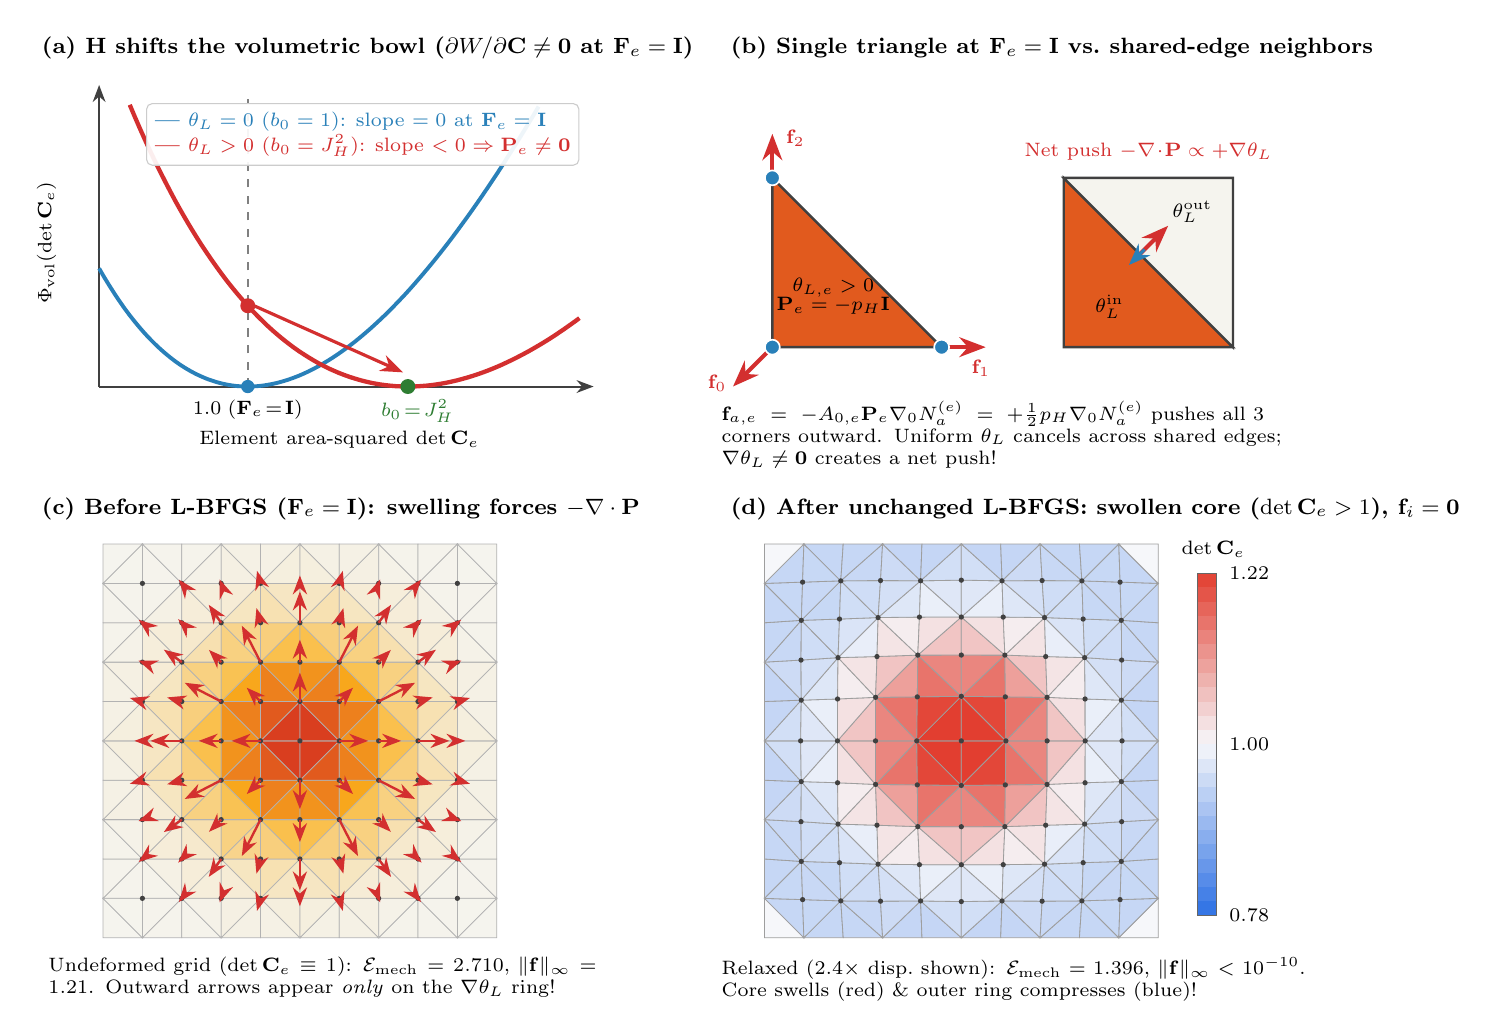
\begin{tikzpicture}[>=Stealth, font=\small]
  \node[anchor=west, font=\bfseries\footnotesize] at (0.0, 12.40) {(a) H shifts the volumetric bowl ($\partial W/\partial\mathbf{C}\neq\mathbf{0}$ at $\mathbf{F}_e=\mathbf{I}$)};
  \draw[->, black!75, line width=0.7pt] (0.850,8.100) -- (7.130,8.100);
  \draw[->, black!75, line width=0.7pt] (0.850,8.100) -- (0.850,11.930);
  \node[anchor=north, font=\scriptsize] at (3.900,7.660) {Element area-squared $\det\mathbf{C}_e$};
  \node[rotate=90, anchor=south, font=\scriptsize] at (0.430,9.925) {$\Phi_{\mathrm{vol}}(\det\mathbf{C}_e)$};
  \draw[dashed, black!50, line width=0.65pt] (2.738,8.100) -- (2.738,11.750);
  \node[anchor=north, font=\scriptsize] at (2.738,8.060) {$1.0\;(\mathbf{F}_e\!=\!\mathbf{I})$};
  \draw[atomblue, line width=1.4pt] (0.850,9.600) -- (0.915,9.488) -- (0.980,9.382) -- (1.045,9.280) -- (1.110,9.183) -- (1.174,9.091) -- (1.239,9.004) -- (1.304,8.922) -- (1.369,8.844) -- (1.434,8.770) -- (1.499,8.701) -- (1.564,8.636) -- (1.629,8.575) -- (1.694,8.518) -- (1.759,8.465) -- (1.823,8.416) -- (1.888,8.371) -- (1.953,8.330) -- (2.018,8.292) -- (2.083,8.258) -- (2.148,8.228) -- (2.213,8.200) -- (2.278,8.177) -- (2.343,8.156) -- (2.407,8.139) -- (2.472,8.125) -- (2.537,8.114) -- (2.602,8.106) -- (2.667,8.102) -- (2.732,8.100) -- (2.797,8.101) -- (2.862,8.105) -- (2.927,8.112) -- (2.991,8.122) -- (3.056,8.134) -- (3.121,8.149) -- (3.186,8.167) -- (3.251,8.187) -- (3.316,8.210) -- (3.381,8.235) -- (3.446,8.263) -- (3.511,8.293) -- (3.576,8.326) -- (3.640,8.360) -- (3.705,8.398) -- (3.770,8.437) -- (3.835,8.479) -- (3.900,8.523) -- (3.965,8.569) -- (4.030,8.617) -- (4.095,8.667) -- (4.160,8.720) -- (4.224,8.774) -- (4.289,8.830) -- (4.354,8.889) -- (4.419,8.949) -- (4.484,9.011) -- (4.549,9.076) -- (4.614,9.142) -- (4.679,9.210) -- (4.744,9.279) -- (4.809,9.351) -- (4.873,9.424) -- (4.938,9.499) -- (5.003,9.576) -- (5.068,9.654) -- (5.133,9.734) -- (5.198,9.816) -- (5.263,9.899) -- (5.328,9.984) -- (5.393,10.071) -- (5.457,10.159) -- (5.522,10.248) -- (5.587,10.339) -- (5.652,10.432) -- (5.717,10.526) -- (5.782,10.622) -- (5.847,10.719) -- (5.912,10.817) -- (5.977,10.917) -- (6.041,11.019) -- (6.106,11.121) -- (6.171,11.225) -- (6.236,11.331) -- (6.301,11.437) -- (6.366,11.545) -- (6.431,11.655);
  \draw[defectred, line width=1.55pt] (1.239,11.678) -- (1.304,11.524) -- (1.369,11.375) -- (1.434,11.230) -- (1.499,11.089) -- (1.564,10.953) -- (1.629,10.821) -- (1.694,10.693) -- (1.759,10.568) -- (1.823,10.448) -- (1.888,10.332) -- (1.953,10.219) -- (2.018,10.110) -- (2.083,10.004) -- (2.148,9.902) -- (2.213,9.804) -- (2.278,9.709) -- (2.343,9.617) -- (2.407,9.529) -- (2.472,9.443) -- (2.537,9.361) -- (2.602,9.282) -- (2.667,9.206) -- (2.732,9.133) -- (2.797,9.063) -- (2.862,8.995) -- (2.927,8.931) -- (2.991,8.869) -- (3.056,8.810) -- (3.121,8.754) -- (3.186,8.700) -- (3.251,8.649) -- (3.316,8.600) -- (3.381,8.554) -- (3.446,8.511) -- (3.511,8.470) -- (3.576,8.431) -- (3.640,8.394) -- (3.705,8.360) -- (3.770,8.328) -- (3.835,8.299) -- (3.900,8.271) -- (3.965,8.246) -- (4.030,8.223) -- (4.095,8.202) -- (4.160,8.183) -- (4.224,8.166) -- (4.289,8.151) -- (4.354,8.138) -- (4.419,8.127) -- (4.484,8.118) -- (4.549,8.111) -- (4.614,8.105) -- (4.679,8.102) -- (4.744,8.100) -- (4.809,8.100) -- (4.873,8.102) -- (4.938,8.106) -- (5.003,8.111) -- (5.068,8.118) -- (5.133,8.127) -- (5.198,8.137) -- (5.263,8.149) -- (5.328,8.163) -- (5.393,8.178) -- (5.457,8.195) -- (5.522,8.213) -- (5.587,8.233) -- (5.652,8.254) -- (5.717,8.277) -- (5.782,8.301) -- (5.847,8.327) -- (5.912,8.354) -- (5.977,8.383) -- (6.041,8.413) -- (6.106,8.444) -- (6.171,8.477) -- (6.236,8.511) -- (6.301,8.546) -- (6.366,8.583) -- (6.431,8.621) -- (6.496,8.660) -- (6.561,8.700) -- (6.626,8.742) -- (6.690,8.785) -- (6.755,8.829) -- (6.820,8.875) -- (6.885,8.921) -- (6.950,8.969);
  \fill[atomblue] (2.738,8.100) circle (2.4pt);
  \fill[defectred] (2.738,9.126) circle (2.7pt);
  \fill[okgreen] (4.771,8.100) circle (2.7pt);
  \node[anchor=north, font=\scriptsize, text=okgreen] at (4.891,8.060) {$b_0\!=\!J_H^2$};
  \draw[->, defectred, line width=1.15pt] (2.818,9.126) -- (4.711,8.280);
  \node[fill=white, fill opacity=0.92, text opacity=1, draw=black!20, rounded corners=2pt, inner sep=3pt, anchor=north east, font=\scriptsize, align=left] at (6.950,11.700) {\textcolor{atomblue}{\textbf{---} $\theta_L=0$ ($b_0=1$): slope $=0$ at $\mathbf{F}_e=\mathbf{I}$}\\[1pt]\textcolor{defectred}{\textbf{---} $\theta_L>0$ ($b_0=J_H^2$): slope $<0 \Rightarrow \mathbf{P}_e\neq\mathbf{0}$}};
  \node[anchor=west, font=\bfseries\footnotesize] at (8.750, 12.40) {(b) Single triangle at $\mathbf{F}_e=\mathbf{I}$ vs.\ shared-edge neighbors};
  \filldraw[fill={rgb,255:red,225;green,90;blue,30}, draw=black!75, line width=0.9pt] (9.400,8.600) -- (11.550,8.600) -- (9.400,10.750) -- cycle;
  \node[font=\scriptsize, align=center] at (10.174,9.245) {$\theta_{L,e}>0$\\[-1pt]$\mathbf{P}_e=-p_H\mathbf{I}$};
  \draw[->, defectred, line width=1.45pt] (9.400,8.600) -- (8.900,8.100);
  \draw[->, defectred, line width=1.45pt] (11.550,8.600) -- (12.110,8.600);
  \draw[->, defectred, line width=1.45pt] (9.400,10.750) -- (9.400,11.310);
  \node[anchor=east, font=\scriptsize, text=defectred] at (8.940,8.140) {$\mathbf{f}_0$};
  \node[anchor=north, font=\scriptsize, text=defectred] at (12.050,8.560) {$\mathbf{f}_1$};
  \node[anchor=west, font=\scriptsize, text=defectred] at (9.450,11.250) {$\mathbf{f}_2$};
  \filldraw[fill=atomblue, draw=white, line width=0.6pt] (9.400,8.600) circle (2.7pt);
  \filldraw[fill=atomblue, draw=white, line width=0.6pt] (11.550,8.600) circle (2.7pt);
  \filldraw[fill=atomblue, draw=white, line width=0.6pt] (9.400,10.750) circle (2.7pt);
  \filldraw[fill={rgb,255:red,225;green,90;blue,30}, draw=black!75, line width=0.85pt] (13.100,8.600) -- (15.250,8.600) -- (13.100,10.750) -- cycle;
  \filldraw[fill={rgb,255:red,245;green,244;blue,238}, draw=black!75, line width=0.85pt] (15.250,10.750) -- (13.100,10.750) -- (15.250,8.600) -- cycle;
  \node[font=\scriptsize] at (13.681,9.116) {$\theta_L^{\mathrm{in}}$};
  \node[font=\scriptsize] at (14.734,10.320) {$\theta_L^{\mathrm{out}}$};
  \draw[->, defectred, line width=1.5pt] (14.017,9.732) -- (14.427,10.142);
  \draw[->, atomblue, line width=1.1pt] (14.127,9.842) -- (13.927,9.642);
  \node[anchor=south, font=\scriptsize, text=defectred] at (14.175,10.850) {Net push $-\nabla\!\cdot\!\mathbf{P}\propto +\nabla\theta_L$};
  \node[anchor=north west, text width=7.5cm, font=\scriptsize, inner sep=0pt] at (8.750, 7.92) {$\mathbf{f}_{a,e}=-A_{0,e}\mathbf{P}_e\nabla_0 N_a^{(e)}=+\frac{1}{2}p_H\nabla_0 N_a^{(e)}$ pushes all 3 corners outward. Uniform $\theta_L$ cancels across shared edges; $\nabla\theta_L\neq\mathbf{0}$ creates a net push!};
  \node[anchor=west, font=\bfseries\footnotesize] at (0.0, 6.55) {(c) Before L-BFGS ($\mathbf{F}_e=\mathbf{I}$): swelling forces $-\nabla\cdot\mathbf{P}$};
  \filldraw[fill={rgb,255:red,245;green,244;blue,238}, draw=black!30, line width=0.28pt] (0.900,1.100) -- (1.400,1.100) -- (0.900,1.600) -- cycle;
  \filldraw[fill={rgb,255:red,245;green,244;blue,237}, draw=black!30, line width=0.28pt] (1.400,1.600) -- (0.900,1.600) -- (1.400,1.100) -- cycle;
  \filldraw[fill={rgb,255:red,245;green,243;blue,236}, draw=black!30, line width=0.28pt] (1.400,1.100) -- (1.900,1.100) -- (1.900,1.600) -- cycle;
  \filldraw[fill={rgb,255:red,245;green,243;blue,236}, draw=black!30, line width=0.28pt] (1.400,1.100) -- (1.900,1.600) -- (1.400,1.600) -- cycle;
  \filldraw[fill={rgb,255:red,245;green,243;blue,235}, draw=black!30, line width=0.28pt] (1.900,1.100) -- (2.400,1.100) -- (1.900,1.600) -- cycle;
  \filldraw[fill={rgb,255:red,245;green,242;blue,232}, draw=black!30, line width=0.28pt] (2.400,1.600) -- (1.900,1.600) -- (2.400,1.100) -- cycle;
  \filldraw[fill={rgb,255:red,245;green,241;blue,229}, draw=black!30, line width=0.28pt] (2.400,1.100) -- (2.900,1.100) -- (2.900,1.600) -- cycle;
  \filldraw[fill={rgb,255:red,245;green,240;blue,227}, draw=black!30, line width=0.28pt] (2.400,1.100) -- (2.900,1.600) -- (2.400,1.600) -- cycle;
  \filldraw[fill={rgb,255:red,245;green,241;blue,229}, draw=black!30, line width=0.28pt] (2.900,1.100) -- (3.400,1.100) -- (2.900,1.600) -- cycle;
  \filldraw[fill={rgb,255:red,245;green,239;blue,222}, draw=black!30, line width=0.28pt] (3.400,1.600) -- (2.900,1.600) -- (3.400,1.100) -- cycle;
  \filldraw[fill={rgb,255:red,245;green,241;blue,229}, draw=black!30, line width=0.28pt] (3.400,1.100) -- (3.900,1.100) -- (3.900,1.600) -- cycle;
  \filldraw[fill={rgb,255:red,245;green,239;blue,222}, draw=black!30, line width=0.28pt] (3.400,1.100) -- (3.900,1.600) -- (3.400,1.600) -- cycle;
  \filldraw[fill={rgb,255:red,245;green,241;blue,229}, draw=black!30, line width=0.28pt] (3.900,1.100) -- (4.400,1.100) -- (3.900,1.600) -- cycle;
  \filldraw[fill={rgb,255:red,245;green,240;blue,227}, draw=black!30, line width=0.28pt] (4.400,1.600) -- (3.900,1.600) -- (4.400,1.100) -- cycle;
  \filldraw[fill={rgb,255:red,245;green,243;blue,235}, draw=black!30, line width=0.28pt] (4.400,1.100) -- (4.900,1.100) -- (4.900,1.600) -- cycle;
  \filldraw[fill={rgb,255:red,245;green,242;blue,232}, draw=black!30, line width=0.28pt] (4.400,1.100) -- (4.900,1.600) -- (4.400,1.600) -- cycle;
  \filldraw[fill={rgb,255:red,245;green,243;blue,236}, draw=black!30, line width=0.28pt] (4.900,1.100) -- (5.400,1.100) -- (4.900,1.600) -- cycle;
  \filldraw[fill={rgb,255:red,245;green,243;blue,236}, draw=black!30, line width=0.28pt] (5.400,1.600) -- (4.900,1.600) -- (5.400,1.100) -- cycle;
  \filldraw[fill={rgb,255:red,245;green,244;blue,238}, draw=black!30, line width=0.28pt] (5.400,1.100) -- (5.900,1.100) -- (5.900,1.600) -- cycle;
  \filldraw[fill={rgb,255:red,245;green,244;blue,237}, draw=black!30, line width=0.28pt] (5.400,1.100) -- (5.900,1.600) -- (5.400,1.600) -- cycle;
  \filldraw[fill={rgb,255:red,245;green,243;blue,236}, draw=black!30, line width=0.28pt] (0.900,1.600) -- (1.400,1.600) -- (1.400,2.100) -- cycle;
  \filldraw[fill={rgb,255:red,245;green,243;blue,236}, draw=black!30, line width=0.28pt] (0.900,1.600) -- (1.400,2.100) -- (0.900,2.100) -- cycle;
  \filldraw[fill={rgb,255:red,245;green,243;blue,235}, draw=black!30, line width=0.28pt] (1.400,1.600) -- (1.900,1.600) -- (1.400,2.100) -- cycle;
  \filldraw[fill={rgb,255:red,245;green,241;blue,229}, draw=black!30, line width=0.28pt] (1.900,2.100) -- (1.400,2.100) -- (1.900,1.600) -- cycle;
  \filldraw[fill={rgb,255:red,246;green,238;blue,219}, draw=black!30, line width=0.28pt] (1.900,1.600) -- (2.400,1.600) -- (2.400,2.100) -- cycle;
  \filldraw[fill={rgb,255:red,246;green,237;blue,217}, draw=black!30, line width=0.28pt] (1.900,1.600) -- (2.400,2.100) -- (1.900,2.100) -- cycle;
  \filldraw[fill={rgb,255:red,246;green,236;blue,214}, draw=black!30, line width=0.28pt] (2.400,1.600) -- (2.900,1.600) -- (2.400,2.100) -- cycle;
  \filldraw[fill={rgb,255:red,246;green,230;blue,193}, draw=black!30, line width=0.28pt] (2.900,2.100) -- (2.400,2.100) -- (2.900,1.600) -- cycle;
  \filldraw[fill={rgb,255:red,246;green,230;blue,195}, draw=black!30, line width=0.28pt] (2.900,1.600) -- (3.400,1.600) -- (3.400,2.100) -- cycle;
  \filldraw[fill={rgb,255:red,247;green,225;blue,178}, draw=black!30, line width=0.28pt] (2.900,1.600) -- (3.400,2.100) -- (2.900,2.100) -- cycle;
  \filldraw[fill={rgb,255:red,246;green,230;blue,195}, draw=black!30, line width=0.28pt] (3.400,1.600) -- (3.900,1.600) -- (3.400,2.100) -- cycle;
  \filldraw[fill={rgb,255:red,247;green,225;blue,178}, draw=black!30, line width=0.28pt] (3.900,2.100) -- (3.400,2.100) -- (3.900,1.600) -- cycle;
  \filldraw[fill={rgb,255:red,246;green,236;blue,214}, draw=black!30, line width=0.28pt] (3.900,1.600) -- (4.400,1.600) -- (4.400,2.100) -- cycle;
  \filldraw[fill={rgb,255:red,246;green,230;blue,193}, draw=black!30, line width=0.28pt] (3.900,1.600) -- (4.400,2.100) -- (3.900,2.100) -- cycle;
  \filldraw[fill={rgb,255:red,246;green,238;blue,219}, draw=black!30, line width=0.28pt] (4.400,1.600) -- (4.900,1.600) -- (4.400,2.100) -- cycle;
  \filldraw[fill={rgb,255:red,246;green,237;blue,217}, draw=black!30, line width=0.28pt] (4.900,2.100) -- (4.400,2.100) -- (4.900,1.600) -- cycle;
  \filldraw[fill={rgb,255:red,245;green,243;blue,235}, draw=black!30, line width=0.28pt] (4.900,1.600) -- (5.400,1.600) -- (5.400,2.100) -- cycle;
  \filldraw[fill={rgb,255:red,245;green,241;blue,229}, draw=black!30, line width=0.28pt] (4.900,1.600) -- (5.400,2.100) -- (4.900,2.100) -- cycle;
  \filldraw[fill={rgb,255:red,245;green,243;blue,236}, draw=black!30, line width=0.28pt] (5.400,1.600) -- (5.900,1.600) -- (5.400,2.100) -- cycle;
  \filldraw[fill={rgb,255:red,245;green,243;blue,236}, draw=black!30, line width=0.28pt] (5.900,2.100) -- (5.400,2.100) -- (5.900,1.600) -- cycle;
  \filldraw[fill={rgb,255:red,245;green,243;blue,235}, draw=black!30, line width=0.28pt] (0.900,2.100) -- (1.400,2.100) -- (0.900,2.600) -- cycle;
  \filldraw[fill={rgb,255:red,245;green,242;blue,232}, draw=black!30, line width=0.28pt] (1.400,2.600) -- (0.900,2.600) -- (1.400,2.100) -- cycle;
  \filldraw[fill={rgb,255:red,246;green,237;blue,217}, draw=black!30, line width=0.28pt] (1.400,2.100) -- (1.900,2.100) -- (1.900,2.600) -- cycle;
  \filldraw[fill={rgb,255:red,246;green,238;blue,219}, draw=black!30, line width=0.28pt] (1.400,2.100) -- (1.900,2.600) -- (1.400,2.600) -- cycle;
  \filldraw[fill={rgb,255:red,246;green,233;blue,205}, draw=black!30, line width=0.28pt] (1.900,2.100) -- (2.400,2.100) -- (1.900,2.600) -- cycle;
  \filldraw[fill={rgb,255:red,247;green,224;blue,176}, draw=black!30, line width=0.28pt] (2.400,2.600) -- (1.900,2.600) -- (2.400,2.100) -- cycle;
  \filldraw[fill={rgb,255:red,248;green,212;blue,140}, draw=black!30, line width=0.28pt] (2.400,2.100) -- (2.900,2.100) -- (2.900,2.600) -- cycle;
  \filldraw[fill={rgb,255:red,248;green,209;blue,129}, draw=black!30, line width=0.28pt] (2.400,2.100) -- (2.900,2.600) -- (2.400,2.600) -- cycle;
  \filldraw[fill={rgb,255:red,248;green,207;blue,125}, draw=black!30, line width=0.28pt] (2.900,2.100) -- (3.400,2.100) -- (2.900,2.600) -- cycle;
  \filldraw[fill={rgb,255:red,250;green,192;blue,77}, draw=black!30, line width=0.28pt] (3.400,2.600) -- (2.900,2.600) -- (3.400,2.100) -- cycle;
  \filldraw[fill={rgb,255:red,248;green,207;blue,125}, draw=black!30, line width=0.28pt] (3.400,2.100) -- (3.900,2.100) -- (3.900,2.600) -- cycle;
  \filldraw[fill={rgb,255:red,250;green,192;blue,77}, draw=black!30, line width=0.28pt] (3.400,2.100) -- (3.900,2.600) -- (3.400,2.600) -- cycle;
  \filldraw[fill={rgb,255:red,248;green,212;blue,140}, draw=black!30, line width=0.28pt] (3.900,2.100) -- (4.400,2.100) -- (3.900,2.600) -- cycle;
  \filldraw[fill={rgb,255:red,248;green,209;blue,129}, draw=black!30, line width=0.28pt] (4.400,2.600) -- (3.900,2.600) -- (4.400,2.100) -- cycle;
  \filldraw[fill={rgb,255:red,246;green,233;blue,205}, draw=black!30, line width=0.28pt] (4.400,2.100) -- (4.900,2.100) -- (4.900,2.600) -- cycle;
  \filldraw[fill={rgb,255:red,247;green,224;blue,176}, draw=black!30, line width=0.28pt] (4.400,2.100) -- (4.900,2.600) -- (4.400,2.600) -- cycle;
  \filldraw[fill={rgb,255:red,246;green,237;blue,217}, draw=black!30, line width=0.28pt] (4.900,2.100) -- (5.400,2.100) -- (4.900,2.600) -- cycle;
  \filldraw[fill={rgb,255:red,246;green,238;blue,219}, draw=black!30, line width=0.28pt] (5.400,2.600) -- (4.900,2.600) -- (5.400,2.100) -- cycle;
  \filldraw[fill={rgb,255:red,245;green,243;blue,235}, draw=black!30, line width=0.28pt] (5.400,2.100) -- (5.900,2.100) -- (5.900,2.600) -- cycle;
  \filldraw[fill={rgb,255:red,245;green,242;blue,232}, draw=black!30, line width=0.28pt] (5.400,2.100) -- (5.900,2.600) -- (5.400,2.600) -- cycle;
  \filldraw[fill={rgb,255:red,245;green,240;blue,227}, draw=black!30, line width=0.28pt] (0.900,2.600) -- (1.400,2.600) -- (1.400,3.100) -- cycle;
  \filldraw[fill={rgb,255:red,245;green,241;blue,229}, draw=black!30, line width=0.28pt] (0.900,2.600) -- (1.400,3.100) -- (0.900,3.100) -- cycle;
  \filldraw[fill={rgb,255:red,246;green,236;blue,214}, draw=black!30, line width=0.28pt] (1.400,2.600) -- (1.900,2.600) -- (1.400,3.100) -- cycle;
  \filldraw[fill={rgb,255:red,246;green,230;blue,193}, draw=black!30, line width=0.28pt] (1.900,3.100) -- (1.400,3.100) -- (1.900,2.600) -- cycle;
  \filldraw[fill={rgb,255:red,248;green,209;blue,129}, draw=black!30, line width=0.28pt] (1.900,2.600) -- (2.400,2.600) -- (2.400,3.100) -- cycle;
  \filldraw[fill={rgb,255:red,248;green,212;blue,140}, draw=black!30, line width=0.28pt] (1.900,2.600) -- (2.400,3.100) -- (1.900,3.100) -- cycle;
  \filldraw[fill={rgb,255:red,249;green,194;blue,83}, draw=black!30, line width=0.28pt] (2.400,2.600) -- (2.900,2.600) -- (2.400,3.100) -- cycle;
  \filldraw[fill={rgb,255:red,248;green,167;blue,28}, draw=black!30, line width=0.28pt] (2.900,3.100) -- (2.400,3.100) -- (2.900,2.600) -- cycle;
  \filldraw[fill={rgb,255:red,242;green,147;blue,29}, draw=black!30, line width=0.28pt] (2.900,2.600) -- (3.400,2.600) -- (3.400,3.100) -- cycle;
  \filldraw[fill={rgb,255:red,237;green,128;blue,29}, draw=black!30, line width=0.28pt] (2.900,2.600) -- (3.400,3.100) -- (2.900,3.100) -- cycle;
  \filldraw[fill={rgb,255:red,242;green,147;blue,29}, draw=black!30, line width=0.28pt] (3.400,2.600) -- (3.900,2.600) -- (3.400,3.100) -- cycle;
  \filldraw[fill={rgb,255:red,237;green,128;blue,29}, draw=black!30, line width=0.28pt] (3.900,3.100) -- (3.400,3.100) -- (3.900,2.600) -- cycle;
  \filldraw[fill={rgb,255:red,249;green,194;blue,83}, draw=black!30, line width=0.28pt] (3.900,2.600) -- (4.400,2.600) -- (4.400,3.100) -- cycle;
  \filldraw[fill={rgb,255:red,248;green,167;blue,28}, draw=black!30, line width=0.28pt] (3.900,2.600) -- (4.400,3.100) -- (3.900,3.100) -- cycle;
  \filldraw[fill={rgb,255:red,248;green,209;blue,129}, draw=black!30, line width=0.28pt] (4.400,2.600) -- (4.900,2.600) -- (4.400,3.100) -- cycle;
  \filldraw[fill={rgb,255:red,248;green,212;blue,140}, draw=black!30, line width=0.28pt] (4.900,3.100) -- (4.400,3.100) -- (4.900,2.600) -- cycle;
  \filldraw[fill={rgb,255:red,246;green,236;blue,214}, draw=black!30, line width=0.28pt] (4.900,2.600) -- (5.400,2.600) -- (5.400,3.100) -- cycle;
  \filldraw[fill={rgb,255:red,246;green,230;blue,193}, draw=black!30, line width=0.28pt] (4.900,2.600) -- (5.400,3.100) -- (4.900,3.100) -- cycle;
  \filldraw[fill={rgb,255:red,245;green,240;blue,227}, draw=black!30, line width=0.28pt] (5.400,2.600) -- (5.900,2.600) -- (5.400,3.100) -- cycle;
  \filldraw[fill={rgb,255:red,245;green,241;blue,229}, draw=black!30, line width=0.28pt] (5.900,3.100) -- (5.400,3.100) -- (5.900,2.600) -- cycle;
  \filldraw[fill={rgb,255:red,245;green,241;blue,229}, draw=black!30, line width=0.28pt] (0.900,3.100) -- (1.400,3.100) -- (0.900,3.600) -- cycle;
  \filldraw[fill={rgb,255:red,245;green,239;blue,222}, draw=black!30, line width=0.28pt] (1.400,3.600) -- (0.900,3.600) -- (1.400,3.100) -- cycle;
  \filldraw[fill={rgb,255:red,247;green,225;blue,178}, draw=black!30, line width=0.28pt] (1.400,3.100) -- (1.900,3.100) -- (1.900,3.600) -- cycle;
  \filldraw[fill={rgb,255:red,246;green,230;blue,195}, draw=black!30, line width=0.28pt] (1.400,3.100) -- (1.900,3.600) -- (1.400,3.600) -- cycle;
  \filldraw[fill={rgb,255:red,248;green,207;blue,125}, draw=black!30, line width=0.28pt] (1.900,3.100) -- (2.400,3.100) -- (1.900,3.600) -- cycle;
  \filldraw[fill={rgb,255:red,250;green,192;blue,77}, draw=black!30, line width=0.28pt] (2.400,3.600) -- (1.900,3.600) -- (2.400,3.100) -- cycle;
  \filldraw[fill={rgb,255:red,237;green,128;blue,29}, draw=black!30, line width=0.28pt] (2.400,3.100) -- (2.900,3.100) -- (2.900,3.600) -- cycle;
  \filldraw[fill={rgb,255:red,242;green,147;blue,29}, draw=black!30, line width=0.28pt] (2.400,3.100) -- (2.900,3.600) -- (2.400,3.600) -- cycle;
  \filldraw[fill={rgb,255:red,225;green,90;blue,30}, draw=black!30, line width=0.28pt] (2.900,3.100) -- (3.400,3.100) -- (2.900,3.600) -- cycle;
  \filldraw[fill={rgb,255:red,217;green,62;blue,31}, draw=black!30, line width=0.28pt] (3.400,3.600) -- (2.900,3.600) -- (3.400,3.100) -- cycle;
  \filldraw[fill={rgb,255:red,225;green,90;blue,30}, draw=black!30, line width=0.28pt] (3.400,3.100) -- (3.900,3.100) -- (3.900,3.600) -- cycle;
  \filldraw[fill={rgb,255:red,217;green,62;blue,31}, draw=black!30, line width=0.28pt] (3.400,3.100) -- (3.900,3.600) -- (3.400,3.600) -- cycle;
  \filldraw[fill={rgb,255:red,237;green,128;blue,29}, draw=black!30, line width=0.28pt] (3.900,3.100) -- (4.400,3.100) -- (3.900,3.600) -- cycle;
  \filldraw[fill={rgb,255:red,242;green,147;blue,29}, draw=black!30, line width=0.28pt] (4.400,3.600) -- (3.900,3.600) -- (4.400,3.100) -- cycle;
  \filldraw[fill={rgb,255:red,248;green,207;blue,125}, draw=black!30, line width=0.28pt] (4.400,3.100) -- (4.900,3.100) -- (4.900,3.600) -- cycle;
  \filldraw[fill={rgb,255:red,250;green,192;blue,77}, draw=black!30, line width=0.28pt] (4.400,3.100) -- (4.900,3.600) -- (4.400,3.600) -- cycle;
  \filldraw[fill={rgb,255:red,247;green,225;blue,178}, draw=black!30, line width=0.28pt] (4.900,3.100) -- (5.400,3.100) -- (4.900,3.600) -- cycle;
  \filldraw[fill={rgb,255:red,246;green,230;blue,195}, draw=black!30, line width=0.28pt] (5.400,3.600) -- (4.900,3.600) -- (5.400,3.100) -- cycle;
  \filldraw[fill={rgb,255:red,245;green,241;blue,229}, draw=black!30, line width=0.28pt] (5.400,3.100) -- (5.900,3.100) -- (5.900,3.600) -- cycle;
  \filldraw[fill={rgb,255:red,245;green,239;blue,222}, draw=black!30, line width=0.28pt] (5.400,3.100) -- (5.900,3.600) -- (5.400,3.600) -- cycle;
  \filldraw[fill={rgb,255:red,245;green,239;blue,222}, draw=black!30, line width=0.28pt] (0.900,3.600) -- (1.400,3.600) -- (1.400,4.100) -- cycle;
  \filldraw[fill={rgb,255:red,245;green,241;blue,229}, draw=black!30, line width=0.28pt] (0.900,3.600) -- (1.400,4.100) -- (0.900,4.100) -- cycle;
  \filldraw[fill={rgb,255:red,246;green,230;blue,195}, draw=black!30, line width=0.28pt] (1.400,3.600) -- (1.900,3.600) -- (1.400,4.100) -- cycle;
  \filldraw[fill={rgb,255:red,247;green,225;blue,178}, draw=black!30, line width=0.28pt] (1.900,4.100) -- (1.400,4.100) -- (1.900,3.600) -- cycle;
  \filldraw[fill={rgb,255:red,250;green,192;blue,77}, draw=black!30, line width=0.28pt] (1.900,3.600) -- (2.400,3.600) -- (2.400,4.100) -- cycle;
  \filldraw[fill={rgb,255:red,248;green,207;blue,125}, draw=black!30, line width=0.28pt] (1.900,3.600) -- (2.400,4.100) -- (1.900,4.100) -- cycle;
  \filldraw[fill={rgb,255:red,242;green,147;blue,29}, draw=black!30, line width=0.28pt] (2.400,3.600) -- (2.900,3.600) -- (2.400,4.100) -- cycle;
  \filldraw[fill={rgb,255:red,237;green,128;blue,29}, draw=black!30, line width=0.28pt] (2.900,4.100) -- (2.400,4.100) -- (2.900,3.600) -- cycle;
  \filldraw[fill={rgb,255:red,217;green,62;blue,31}, draw=black!30, line width=0.28pt] (2.900,3.600) -- (3.400,3.600) -- (3.400,4.100) -- cycle;
  \filldraw[fill={rgb,255:red,225;green,90;blue,30}, draw=black!30, line width=0.28pt] (2.900,3.600) -- (3.400,4.100) -- (2.900,4.100) -- cycle;
  \filldraw[fill={rgb,255:red,217;green,62;blue,31}, draw=black!30, line width=0.28pt] (3.400,3.600) -- (3.900,3.600) -- (3.400,4.100) -- cycle;
  \filldraw[fill={rgb,255:red,225;green,90;blue,30}, draw=black!30, line width=0.28pt] (3.900,4.100) -- (3.400,4.100) -- (3.900,3.600) -- cycle;
  \filldraw[fill={rgb,255:red,242;green,147;blue,29}, draw=black!30, line width=0.28pt] (3.900,3.600) -- (4.400,3.600) -- (4.400,4.100) -- cycle;
  \filldraw[fill={rgb,255:red,237;green,128;blue,29}, draw=black!30, line width=0.28pt] (3.900,3.600) -- (4.400,4.100) -- (3.900,4.100) -- cycle;
  \filldraw[fill={rgb,255:red,250;green,192;blue,77}, draw=black!30, line width=0.28pt] (4.400,3.600) -- (4.900,3.600) -- (4.400,4.100) -- cycle;
  \filldraw[fill={rgb,255:red,248;green,207;blue,125}, draw=black!30, line width=0.28pt] (4.900,4.100) -- (4.400,4.100) -- (4.900,3.600) -- cycle;
  \filldraw[fill={rgb,255:red,246;green,230;blue,195}, draw=black!30, line width=0.28pt] (4.900,3.600) -- (5.400,3.600) -- (5.400,4.100) -- cycle;
  \filldraw[fill={rgb,255:red,247;green,225;blue,178}, draw=black!30, line width=0.28pt] (4.900,3.600) -- (5.400,4.100) -- (4.900,4.100) -- cycle;
  \filldraw[fill={rgb,255:red,245;green,239;blue,222}, draw=black!30, line width=0.28pt] (5.400,3.600) -- (5.900,3.600) -- (5.400,4.100) -- cycle;
  \filldraw[fill={rgb,255:red,245;green,241;blue,229}, draw=black!30, line width=0.28pt] (5.900,4.100) -- (5.400,4.100) -- (5.900,3.600) -- cycle;
  \filldraw[fill={rgb,255:red,245;green,241;blue,229}, draw=black!30, line width=0.28pt] (0.900,4.100) -- (1.400,4.100) -- (0.900,4.600) -- cycle;
  \filldraw[fill={rgb,255:red,245;green,240;blue,227}, draw=black!30, line width=0.28pt] (1.400,4.600) -- (0.900,4.600) -- (1.400,4.100) -- cycle;
  \filldraw[fill={rgb,255:red,246;green,230;blue,193}, draw=black!30, line width=0.28pt] (1.400,4.100) -- (1.900,4.100) -- (1.900,4.600) -- cycle;
  \filldraw[fill={rgb,255:red,246;green,236;blue,214}, draw=black!30, line width=0.28pt] (1.400,4.100) -- (1.900,4.600) -- (1.400,4.600) -- cycle;
  \filldraw[fill={rgb,255:red,248;green,212;blue,140}, draw=black!30, line width=0.28pt] (1.900,4.100) -- (2.400,4.100) -- (1.900,4.600) -- cycle;
  \filldraw[fill={rgb,255:red,248;green,209;blue,129}, draw=black!30, line width=0.28pt] (2.400,4.600) -- (1.900,4.600) -- (2.400,4.100) -- cycle;
  \filldraw[fill={rgb,255:red,248;green,167;blue,28}, draw=black!30, line width=0.28pt] (2.400,4.100) -- (2.900,4.100) -- (2.900,4.600) -- cycle;
  \filldraw[fill={rgb,255:red,249;green,194;blue,83}, draw=black!30, line width=0.28pt] (2.400,4.100) -- (2.900,4.600) -- (2.400,4.600) -- cycle;
  \filldraw[fill={rgb,255:red,237;green,128;blue,29}, draw=black!30, line width=0.28pt] (2.900,4.100) -- (3.400,4.100) -- (2.900,4.600) -- cycle;
  \filldraw[fill={rgb,255:red,242;green,147;blue,29}, draw=black!30, line width=0.28pt] (3.400,4.600) -- (2.900,4.600) -- (3.400,4.100) -- cycle;
  \filldraw[fill={rgb,255:red,237;green,128;blue,29}, draw=black!30, line width=0.28pt] (3.400,4.100) -- (3.900,4.100) -- (3.900,4.600) -- cycle;
  \filldraw[fill={rgb,255:red,242;green,147;blue,29}, draw=black!30, line width=0.28pt] (3.400,4.100) -- (3.900,4.600) -- (3.400,4.600) -- cycle;
  \filldraw[fill={rgb,255:red,248;green,167;blue,28}, draw=black!30, line width=0.28pt] (3.900,4.100) -- (4.400,4.100) -- (3.900,4.600) -- cycle;
  \filldraw[fill={rgb,255:red,249;green,194;blue,83}, draw=black!30, line width=0.28pt] (4.400,4.600) -- (3.900,4.600) -- (4.400,4.100) -- cycle;
  \filldraw[fill={rgb,255:red,248;green,212;blue,140}, draw=black!30, line width=0.28pt] (4.400,4.100) -- (4.900,4.100) -- (4.900,4.600) -- cycle;
  \filldraw[fill={rgb,255:red,248;green,209;blue,129}, draw=black!30, line width=0.28pt] (4.400,4.100) -- (4.900,4.600) -- (4.400,4.600) -- cycle;
  \filldraw[fill={rgb,255:red,246;green,230;blue,193}, draw=black!30, line width=0.28pt] (4.900,4.100) -- (5.400,4.100) -- (4.900,4.600) -- cycle;
  \filldraw[fill={rgb,255:red,246;green,236;blue,214}, draw=black!30, line width=0.28pt] (5.400,4.600) -- (4.900,4.600) -- (5.400,4.100) -- cycle;
  \filldraw[fill={rgb,255:red,245;green,241;blue,229}, draw=black!30, line width=0.28pt] (5.400,4.100) -- (5.900,4.100) -- (5.900,4.600) -- cycle;
  \filldraw[fill={rgb,255:red,245;green,240;blue,227}, draw=black!30, line width=0.28pt] (5.400,4.100) -- (5.900,4.600) -- (5.400,4.600) -- cycle;
  \filldraw[fill={rgb,255:red,245;green,242;blue,232}, draw=black!30, line width=0.28pt] (0.900,4.600) -- (1.400,4.600) -- (1.400,5.100) -- cycle;
  \filldraw[fill={rgb,255:red,245;green,243;blue,235}, draw=black!30, line width=0.28pt] (0.900,4.600) -- (1.400,5.100) -- (0.900,5.100) -- cycle;
  \filldraw[fill={rgb,255:red,246;green,238;blue,219}, draw=black!30, line width=0.28pt] (1.400,4.600) -- (1.900,4.600) -- (1.400,5.100) -- cycle;
  \filldraw[fill={rgb,255:red,246;green,237;blue,217}, draw=black!30, line width=0.28pt] (1.900,5.100) -- (1.400,5.100) -- (1.900,4.600) -- cycle;
  \filldraw[fill={rgb,255:red,247;green,224;blue,176}, draw=black!30, line width=0.28pt] (1.900,4.600) -- (2.400,4.600) -- (2.400,5.100) -- cycle;
  \filldraw[fill={rgb,255:red,246;green,233;blue,205}, draw=black!30, line width=0.28pt] (1.900,4.600) -- (2.400,5.100) -- (1.900,5.100) -- cycle;
  \filldraw[fill={rgb,255:red,248;green,209;blue,129}, draw=black!30, line width=0.28pt] (2.400,4.600) -- (2.900,4.600) -- (2.400,5.100) -- cycle;
  \filldraw[fill={rgb,255:red,248;green,212;blue,140}, draw=black!30, line width=0.28pt] (2.900,5.100) -- (2.400,5.100) -- (2.900,4.600) -- cycle;
  \filldraw[fill={rgb,255:red,250;green,192;blue,77}, draw=black!30, line width=0.28pt] (2.900,4.600) -- (3.400,4.600) -- (3.400,5.100) -- cycle;
  \filldraw[fill={rgb,255:red,248;green,207;blue,125}, draw=black!30, line width=0.28pt] (2.900,4.600) -- (3.400,5.100) -- (2.900,5.100) -- cycle;
  \filldraw[fill={rgb,255:red,250;green,192;blue,77}, draw=black!30, line width=0.28pt] (3.400,4.600) -- (3.900,4.600) -- (3.400,5.100) -- cycle;
  \filldraw[fill={rgb,255:red,248;green,207;blue,125}, draw=black!30, line width=0.28pt] (3.900,5.100) -- (3.400,5.100) -- (3.900,4.600) -- cycle;
  \filldraw[fill={rgb,255:red,248;green,209;blue,129}, draw=black!30, line width=0.28pt] (3.900,4.600) -- (4.400,4.600) -- (4.400,5.100) -- cycle;
  \filldraw[fill={rgb,255:red,248;green,212;blue,140}, draw=black!30, line width=0.28pt] (3.900,4.600) -- (4.400,5.100) -- (3.900,5.100) -- cycle;
  \filldraw[fill={rgb,255:red,247;green,224;blue,176}, draw=black!30, line width=0.28pt] (4.400,4.600) -- (4.900,4.600) -- (4.400,5.100) -- cycle;
  \filldraw[fill={rgb,255:red,246;green,233;blue,205}, draw=black!30, line width=0.28pt] (4.900,5.100) -- (4.400,5.100) -- (4.900,4.600) -- cycle;
  \filldraw[fill={rgb,255:red,246;green,238;blue,219}, draw=black!30, line width=0.28pt] (4.900,4.600) -- (5.400,4.600) -- (5.400,5.100) -- cycle;
  \filldraw[fill={rgb,255:red,246;green,237;blue,217}, draw=black!30, line width=0.28pt] (4.900,4.600) -- (5.400,5.100) -- (4.900,5.100) -- cycle;
  \filldraw[fill={rgb,255:red,245;green,242;blue,232}, draw=black!30, line width=0.28pt] (5.400,4.600) -- (5.900,4.600) -- (5.400,5.100) -- cycle;
  \filldraw[fill={rgb,255:red,245;green,243;blue,235}, draw=black!30, line width=0.28pt] (5.900,5.100) -- (5.400,5.100) -- (5.900,4.600) -- cycle;
  \filldraw[fill={rgb,255:red,245;green,243;blue,236}, draw=black!30, line width=0.28pt] (0.900,5.100) -- (1.400,5.100) -- (0.900,5.600) -- cycle;
  \filldraw[fill={rgb,255:red,245;green,243;blue,236}, draw=black!30, line width=0.28pt] (1.400,5.600) -- (0.900,5.600) -- (1.400,5.100) -- cycle;
  \filldraw[fill={rgb,255:red,245;green,241;blue,229}, draw=black!30, line width=0.28pt] (1.400,5.100) -- (1.900,5.100) -- (1.900,5.600) -- cycle;
  \filldraw[fill={rgb,255:red,245;green,243;blue,235}, draw=black!30, line width=0.28pt] (1.400,5.100) -- (1.900,5.600) -- (1.400,5.600) -- cycle;
  \filldraw[fill={rgb,255:red,246;green,237;blue,217}, draw=black!30, line width=0.28pt] (1.900,5.100) -- (2.400,5.100) -- (1.900,5.600) -- cycle;
  \filldraw[fill={rgb,255:red,246;green,238;blue,219}, draw=black!30, line width=0.28pt] (2.400,5.600) -- (1.900,5.600) -- (2.400,5.100) -- cycle;
  \filldraw[fill={rgb,255:red,246;green,230;blue,193}, draw=black!30, line width=0.28pt] (2.400,5.100) -- (2.900,5.100) -- (2.900,5.600) -- cycle;
  \filldraw[fill={rgb,255:red,246;green,236;blue,214}, draw=black!30, line width=0.28pt] (2.400,5.100) -- (2.900,5.600) -- (2.400,5.600) -- cycle;
  \filldraw[fill={rgb,255:red,247;green,225;blue,178}, draw=black!30, line width=0.28pt] (2.900,5.100) -- (3.400,5.100) -- (2.900,5.600) -- cycle;
  \filldraw[fill={rgb,255:red,246;green,230;blue,195}, draw=black!30, line width=0.28pt] (3.400,5.600) -- (2.900,5.600) -- (3.400,5.100) -- cycle;
  \filldraw[fill={rgb,255:red,247;green,225;blue,178}, draw=black!30, line width=0.28pt] (3.400,5.100) -- (3.900,5.100) -- (3.900,5.600) -- cycle;
  \filldraw[fill={rgb,255:red,246;green,230;blue,195}, draw=black!30, line width=0.28pt] (3.400,5.100) -- (3.900,5.600) -- (3.400,5.600) -- cycle;
  \filldraw[fill={rgb,255:red,246;green,230;blue,193}, draw=black!30, line width=0.28pt] (3.900,5.100) -- (4.400,5.100) -- (3.900,5.600) -- cycle;
  \filldraw[fill={rgb,255:red,246;green,236;blue,214}, draw=black!30, line width=0.28pt] (4.400,5.600) -- (3.900,5.600) -- (4.400,5.100) -- cycle;
  \filldraw[fill={rgb,255:red,246;green,237;blue,217}, draw=black!30, line width=0.28pt] (4.400,5.100) -- (4.900,5.100) -- (4.900,5.600) -- cycle;
  \filldraw[fill={rgb,255:red,246;green,238;blue,219}, draw=black!30, line width=0.28pt] (4.400,5.100) -- (4.900,5.600) -- (4.400,5.600) -- cycle;
  \filldraw[fill={rgb,255:red,245;green,241;blue,229}, draw=black!30, line width=0.28pt] (4.900,5.100) -- (5.400,5.100) -- (4.900,5.600) -- cycle;
  \filldraw[fill={rgb,255:red,245;green,243;blue,235}, draw=black!30, line width=0.28pt] (5.400,5.600) -- (4.900,5.600) -- (5.400,5.100) -- cycle;
  \filldraw[fill={rgb,255:red,245;green,243;blue,236}, draw=black!30, line width=0.28pt] (5.400,5.100) -- (5.900,5.100) -- (5.900,5.600) -- cycle;
  \filldraw[fill={rgb,255:red,245;green,243;blue,236}, draw=black!30, line width=0.28pt] (5.400,5.100) -- (5.900,5.600) -- (5.400,5.600) -- cycle;
  \filldraw[fill={rgb,255:red,245;green,244;blue,237}, draw=black!30, line width=0.28pt] (0.900,5.600) -- (1.400,5.600) -- (1.400,6.100) -- cycle;
  \filldraw[fill={rgb,255:red,245;green,244;blue,238}, draw=black!30, line width=0.28pt] (0.900,5.600) -- (1.400,6.100) -- (0.900,6.100) -- cycle;
  \filldraw[fill={rgb,255:red,245;green,243;blue,236}, draw=black!30, line width=0.28pt] (1.400,5.600) -- (1.900,5.600) -- (1.400,6.100) -- cycle;
  \filldraw[fill={rgb,255:red,245;green,243;blue,236}, draw=black!30, line width=0.28pt] (1.900,6.100) -- (1.400,6.100) -- (1.900,5.600) -- cycle;
  \filldraw[fill={rgb,255:red,245;green,242;blue,232}, draw=black!30, line width=0.28pt] (1.900,5.600) -- (2.400,5.600) -- (2.400,6.100) -- cycle;
  \filldraw[fill={rgb,255:red,245;green,243;blue,235}, draw=black!30, line width=0.28pt] (1.900,5.600) -- (2.400,6.100) -- (1.900,6.100) -- cycle;
  \filldraw[fill={rgb,255:red,245;green,240;blue,227}, draw=black!30, line width=0.28pt] (2.400,5.600) -- (2.900,5.600) -- (2.400,6.100) -- cycle;
  \filldraw[fill={rgb,255:red,245;green,241;blue,229}, draw=black!30, line width=0.28pt] (2.900,6.100) -- (2.400,6.100) -- (2.900,5.600) -- cycle;
  \filldraw[fill={rgb,255:red,245;green,239;blue,222}, draw=black!30, line width=0.28pt] (2.900,5.600) -- (3.400,5.600) -- (3.400,6.100) -- cycle;
  \filldraw[fill={rgb,255:red,245;green,241;blue,229}, draw=black!30, line width=0.28pt] (2.900,5.600) -- (3.400,6.100) -- (2.900,6.100) -- cycle;
  \filldraw[fill={rgb,255:red,245;green,239;blue,222}, draw=black!30, line width=0.28pt] (3.400,5.600) -- (3.900,5.600) -- (3.400,6.100) -- cycle;
  \filldraw[fill={rgb,255:red,245;green,241;blue,229}, draw=black!30, line width=0.28pt] (3.900,6.100) -- (3.400,6.100) -- (3.900,5.600) -- cycle;
  \filldraw[fill={rgb,255:red,245;green,240;blue,227}, draw=black!30, line width=0.28pt] (3.900,5.600) -- (4.400,5.600) -- (4.400,6.100) -- cycle;
  \filldraw[fill={rgb,255:red,245;green,241;blue,229}, draw=black!30, line width=0.28pt] (3.900,5.600) -- (4.400,6.100) -- (3.900,6.100) -- cycle;
  \filldraw[fill={rgb,255:red,245;green,242;blue,232}, draw=black!30, line width=0.28pt] (4.400,5.600) -- (4.900,5.600) -- (4.400,6.100) -- cycle;
  \filldraw[fill={rgb,255:red,245;green,243;blue,235}, draw=black!30, line width=0.28pt] (4.900,6.100) -- (4.400,6.100) -- (4.900,5.600) -- cycle;
  \filldraw[fill={rgb,255:red,245;green,243;blue,236}, draw=black!30, line width=0.28pt] (4.900,5.600) -- (5.400,5.600) -- (5.400,6.100) -- cycle;
  \filldraw[fill={rgb,255:red,245;green,243;blue,236}, draw=black!30, line width=0.28pt] (4.900,5.600) -- (5.400,6.100) -- (4.900,6.100) -- cycle;
  \filldraw[fill={rgb,255:red,245;green,244;blue,237}, draw=black!30, line width=0.28pt] (5.400,5.600) -- (5.900,5.600) -- (5.400,6.100) -- cycle;
  \filldraw[fill={rgb,255:red,245;green,244;blue,238}, draw=black!30, line width=0.28pt] (5.900,6.100) -- (5.400,6.100) -- (5.900,5.600) -- cycle;
  \fill[black!75] (1.400,1.600) circle (0.95pt);
  \fill[black!75] (1.900,1.600) circle (0.95pt);
  \draw[->, defectred, line width=0.85pt] (1.900,1.600) -- (1.862,1.552);
  \fill[black!75] (2.400,1.600) circle (0.95pt);
  \draw[->, defectred, line width=0.85pt] (2.400,1.600) -- (2.381,1.550);
  \fill[black!75] (2.900,1.600) circle (0.95pt);
  \draw[->, defectred, line width=0.85pt] (2.900,1.600) -- (2.855,1.441);
  \fill[black!75] (3.400,1.600) circle (0.95pt);
  \draw[->, defectred, line width=0.85pt] (3.400,1.600) -- (3.400,1.499);
  \fill[black!75] (3.900,1.600) circle (0.95pt);
  \draw[->, defectred, line width=0.85pt] (3.900,1.600) -- (3.945,1.441);
  \fill[black!75] (4.400,1.600) circle (0.95pt);
  \draw[->, defectred, line width=0.85pt] (4.400,1.600) -- (4.419,1.550);
  \fill[black!75] (4.900,1.600) circle (0.95pt);
  \draw[->, defectred, line width=0.85pt] (4.900,1.600) -- (4.938,1.552);
  \fill[black!75] (5.400,1.600) circle (0.95pt);
  \fill[black!75] (1.400,2.100) circle (0.95pt);
  \draw[->, defectred, line width=0.85pt] (1.400,2.100) -- (1.352,2.062);
  \fill[black!75] (1.900,2.100) circle (0.95pt);
  \draw[->, defectred, line width=0.85pt] (1.900,2.100) -- (1.854,2.054);
  \fill[black!75] (2.400,2.100) circle (0.95pt);
  \draw[->, defectred, line width=0.85pt] (2.400,2.100) -- (2.242,1.872);
  \fill[black!75] (2.900,2.100) circle (0.95pt);
  \draw[->, defectred, line width=0.85pt] (2.900,2.100) -- (2.848,1.914);
  \fill[black!75] (3.400,2.100) circle (0.95pt);
  \draw[->, defectred, line width=0.85pt] (3.400,2.100) -- (3.400,1.702);
  \fill[black!75] (3.900,2.100) circle (0.95pt);
  \draw[->, defectred, line width=0.85pt] (3.900,2.100) -- (3.952,1.914);
  \fill[black!75] (4.400,2.100) circle (0.95pt);
  \draw[->, defectred, line width=0.85pt] (4.400,2.100) -- (4.558,1.872);
  \fill[black!75] (4.900,2.100) circle (0.95pt);
  \draw[->, defectred, line width=0.85pt] (4.900,2.100) -- (4.946,2.054);
  \fill[black!75] (5.400,2.100) circle (0.95pt);
  \draw[->, defectred, line width=0.85pt] (5.400,2.100) -- (5.448,2.062);
  \fill[black!75] (1.400,2.600) circle (0.95pt);
  \draw[->, defectred, line width=0.85pt] (1.400,2.600) -- (1.350,2.581);
  \fill[black!75] (1.900,2.600) circle (0.95pt);
  \draw[->, defectred, line width=0.85pt] (1.900,2.600) -- (1.672,2.442);
  \fill[black!75] (2.400,2.600) circle (0.95pt);
  \draw[->, defectred, line width=0.85pt] (2.400,2.600) -- (2.245,2.445);
  \fill[black!75] (2.900,2.600) circle (0.95pt);
  \draw[->, defectred, line width=0.85pt] (2.900,2.600) -- (2.662,2.137);
  \fill[black!75] (3.400,2.600) circle (0.95pt);
  \draw[->, defectred, line width=0.85pt] (3.400,2.600) -- (3.400,2.315);
  \fill[black!75] (3.900,2.600) circle (0.95pt);
  \draw[->, defectred, line width=0.85pt] (3.900,2.600) -- (4.138,2.137);
  \fill[black!75] (4.400,2.600) circle (0.95pt);
  \draw[->, defectred, line width=0.85pt] (4.400,2.600) -- (4.555,2.445);
  \fill[black!75] (4.900,2.600) circle (0.95pt);
  \draw[->, defectred, line width=0.85pt] (4.900,2.600) -- (5.128,2.442);
  \fill[black!75] (5.400,2.600) circle (0.95pt);
  \draw[->, defectred, line width=0.85pt] (5.400,2.600) -- (5.450,2.581);
  \fill[black!75] (1.400,3.100) circle (0.95pt);
  \draw[->, defectred, line width=0.85pt] (1.400,3.100) -- (1.241,3.055);
  \fill[black!75] (1.900,3.100) circle (0.95pt);
  \draw[->, defectred, line width=0.85pt] (1.900,3.100) -- (1.714,3.048);
  \fill[black!75] (2.400,3.100) circle (0.95pt);
  \draw[->, defectred, line width=0.85pt] (2.400,3.100) -- (1.937,2.862);
  \fill[black!75] (2.900,3.100) circle (0.95pt);
  \draw[->, defectred, line width=0.85pt] (2.900,3.100) -- (2.725,2.925);
  \fill[black!75] (3.400,3.100) circle (0.95pt);
  \draw[->, defectred, line width=0.85pt] (3.400,3.100) -- (3.400,2.733);
  \fill[black!75] (3.900,3.100) circle (0.95pt);
  \draw[->, defectred, line width=0.85pt] (3.900,3.100) -- (4.075,2.925);
  \fill[black!75] (4.400,3.100) circle (0.95pt);
  \draw[->, defectred, line width=0.85pt] (4.400,3.100) -- (4.863,2.862);
  \fill[black!75] (4.900,3.100) circle (0.95pt);
  \draw[->, defectred, line width=0.85pt] (4.900,3.100) -- (5.086,3.048);
  \fill[black!75] (5.400,3.100) circle (0.95pt);
  \draw[->, defectred, line width=0.85pt] (5.400,3.100) -- (5.559,3.055);
  \fill[black!75] (1.400,3.600) circle (0.95pt);
  \draw[->, defectred, line width=0.85pt] (1.400,3.600) -- (1.299,3.600);
  \fill[black!75] (1.900,3.600) circle (0.95pt);
  \draw[->, defectred, line width=0.85pt] (1.900,3.600) -- (1.502,3.600);
  \fill[black!75] (2.400,3.600) circle (0.95pt);
  \draw[->, defectred, line width=0.85pt] (2.400,3.600) -- (2.115,3.600);
  \fill[black!75] (2.900,3.600) circle (0.95pt);
  \draw[->, defectred, line width=0.85pt] (2.900,3.600) -- (2.533,3.600);
  \fill[black!75] (3.400,3.600) circle (0.95pt);
  \fill[black!75] (3.900,3.600) circle (0.95pt);
  \draw[->, defectred, line width=0.85pt] (3.900,3.600) -- (4.267,3.600);
  \fill[black!75] (4.400,3.600) circle (0.95pt);
  \draw[->, defectred, line width=0.85pt] (4.400,3.600) -- (4.685,3.600);
  \fill[black!75] (4.900,3.600) circle (0.95pt);
  \draw[->, defectred, line width=0.85pt] (4.900,3.600) -- (5.298,3.600);
  \fill[black!75] (5.400,3.600) circle (0.95pt);
  \draw[->, defectred, line width=0.85pt] (5.400,3.600) -- (5.501,3.600);
  \fill[black!75] (1.400,4.100) circle (0.95pt);
  \draw[->, defectred, line width=0.85pt] (1.400,4.100) -- (1.241,4.145);
  \fill[black!75] (1.900,4.100) circle (0.95pt);
  \draw[->, defectred, line width=0.85pt] (1.900,4.100) -- (1.714,4.152);
  \fill[black!75] (2.400,4.100) circle (0.95pt);
  \draw[->, defectred, line width=0.85pt] (2.400,4.100) -- (1.937,4.338);
  \fill[black!75] (2.900,4.100) circle (0.95pt);
  \draw[->, defectred, line width=0.85pt] (2.900,4.100) -- (2.725,4.275);
  \fill[black!75] (3.400,4.100) circle (0.95pt);
  \draw[->, defectred, line width=0.85pt] (3.400,4.100) -- (3.400,4.467);
  \fill[black!75] (3.900,4.100) circle (0.95pt);
  \draw[->, defectred, line width=0.85pt] (3.900,4.100) -- (4.075,4.275);
  \fill[black!75] (4.400,4.100) circle (0.95pt);
  \draw[->, defectred, line width=0.85pt] (4.400,4.100) -- (4.863,4.338);
  \fill[black!75] (4.900,4.100) circle (0.95pt);
  \draw[->, defectred, line width=0.85pt] (4.900,4.100) -- (5.086,4.152);
  \fill[black!75] (5.400,4.100) circle (0.95pt);
  \draw[->, defectred, line width=0.85pt] (5.400,4.100) -- (5.559,4.145);
  \fill[black!75] (1.400,4.600) circle (0.95pt);
  \draw[->, defectred, line width=0.85pt] (1.400,4.600) -- (1.350,4.619);
  \fill[black!75] (1.900,4.600) circle (0.95pt);
  \draw[->, defectred, line width=0.85pt] (1.900,4.600) -- (1.672,4.758);
  \fill[black!75] (2.400,4.600) circle (0.95pt);
  \draw[->, defectred, line width=0.85pt] (2.400,4.600) -- (2.245,4.755);
  \fill[black!75] (2.900,4.600) circle (0.95pt);
  \draw[->, defectred, line width=0.85pt] (2.900,4.600) -- (2.662,5.063);
  \fill[black!75] (3.400,4.600) circle (0.95pt);
  \draw[->, defectred, line width=0.85pt] (3.400,4.600) -- (3.400,4.885);
  \fill[black!75] (3.900,4.600) circle (0.95pt);
  \draw[->, defectred, line width=0.85pt] (3.900,4.600) -- (4.138,5.063);
  \fill[black!75] (4.400,4.600) circle (0.95pt);
  \draw[->, defectred, line width=0.85pt] (4.400,4.600) -- (4.555,4.755);
  \fill[black!75] (4.900,4.600) circle (0.95pt);
  \draw[->, defectred, line width=0.85pt] (4.900,4.600) -- (5.128,4.758);
  \fill[black!75] (5.400,4.600) circle (0.95pt);
  \draw[->, defectred, line width=0.85pt] (5.400,4.600) -- (5.450,4.619);
  \fill[black!75] (1.400,5.100) circle (0.95pt);
  \draw[->, defectred, line width=0.85pt] (1.400,5.100) -- (1.352,5.138);
  \fill[black!75] (1.900,5.100) circle (0.95pt);
  \draw[->, defectred, line width=0.85pt] (1.900,5.100) -- (1.854,5.146);
  \fill[black!75] (2.400,5.100) circle (0.95pt);
  \draw[->, defectred, line width=0.85pt] (2.400,5.100) -- (2.242,5.328);
  \fill[black!75] (2.900,5.100) circle (0.95pt);
  \draw[->, defectred, line width=0.85pt] (2.900,5.100) -- (2.848,5.286);
  \fill[black!75] (3.400,5.100) circle (0.95pt);
  \draw[->, defectred, line width=0.85pt] (3.400,5.100) -- (3.400,5.498);
  \fill[black!75] (3.900,5.100) circle (0.95pt);
  \draw[->, defectred, line width=0.85pt] (3.900,5.100) -- (3.952,5.286);
  \fill[black!75] (4.400,5.100) circle (0.95pt);
  \draw[->, defectred, line width=0.85pt] (4.400,5.100) -- (4.558,5.328);
  \fill[black!75] (4.900,5.100) circle (0.95pt);
  \draw[->, defectred, line width=0.85pt] (4.900,5.100) -- (4.946,5.146);
  \fill[black!75] (5.400,5.100) circle (0.95pt);
  \draw[->, defectred, line width=0.85pt] (5.400,5.100) -- (5.448,5.138);
  \fill[black!75] (1.400,5.600) circle (0.95pt);
  \fill[black!75] (1.900,5.600) circle (0.95pt);
  \draw[->, defectred, line width=0.85pt] (1.900,5.600) -- (1.862,5.648);
  \fill[black!75] (2.400,5.600) circle (0.95pt);
  \draw[->, defectred, line width=0.85pt] (2.400,5.600) -- (2.381,5.650);
  \fill[black!75] (2.900,5.600) circle (0.95pt);
  \draw[->, defectred, line width=0.85pt] (2.900,5.600) -- (2.855,5.759);
  \fill[black!75] (3.400,5.600) circle (0.95pt);
  \draw[->, defectred, line width=0.85pt] (3.400,5.600) -- (3.400,5.701);
  \fill[black!75] (3.900,5.600) circle (0.95pt);
  \draw[->, defectred, line width=0.85pt] (3.900,5.600) -- (3.945,5.759);
  \fill[black!75] (4.400,5.600) circle (0.95pt);
  \draw[->, defectred, line width=0.85pt] (4.400,5.600) -- (4.419,5.650);
  \fill[black!75] (4.900,5.600) circle (0.95pt);
  \draw[->, defectred, line width=0.85pt] (4.900,5.600) -- (4.938,5.648);
  \fill[black!75] (5.400,5.600) circle (0.95pt);
  \node[anchor=north west, font=\scriptsize, text width=7.2cm, inner sep=0pt] at (0.20, 0.86) {Undeformed grid ($\det\mathbf{C}_e\equiv 1$): $\mathcal{E}_{\mathrm{mech}}=2.710$, $\|\mathbf{f}\|_\infty=1.21$. Outward arrows appear \emph{only} on the $\nabla\theta_L$ ring!};
  \node[anchor=west, font=\bfseries\footnotesize] at (8.750, 6.55) {(d) After unchanged L-BFGS: swollen core ($\det\mathbf{C}_e>1$), $\mathbf{f}_i=\mathbf{0}$};
  \filldraw[fill={rgb,255:red,246;green,247;blue,250}, draw=black!38, line width=0.30pt] (9.300,1.100) -- (9.800,1.100) -- (9.300,1.600) -- cycle;
  \filldraw[fill={rgb,255:red,198;green,215;blue,245}, draw=black!38, line width=0.30pt] (9.784,1.584) -- (9.300,1.600) -- (9.800,1.100) -- cycle;
  \filldraw[fill={rgb,255:red,198;green,215;blue,245}, draw=black!38, line width=0.30pt] (9.800,1.100) -- (10.300,1.100) -- (10.269,1.568) -- cycle;
  \filldraw[fill={rgb,255:red,199;green,216;blue,245}, draw=black!38, line width=0.30pt] (9.800,1.100) -- (10.269,1.568) -- (9.784,1.584) -- cycle;
  \filldraw[fill={rgb,255:red,198;green,215;blue,245}, draw=black!38, line width=0.30pt] (10.300,1.100) -- (10.800,1.100) -- (10.269,1.568) -- cycle;
  \filldraw[fill={rgb,255:red,200;green,216;blue,245}, draw=black!38, line width=0.30pt] (10.774,1.564) -- (10.269,1.568) -- (10.800,1.100) -- cycle;
  \filldraw[fill={rgb,255:red,197;green,214;blue,245}, draw=black!38, line width=0.30pt] (10.800,1.100) -- (11.300,1.100) -- (11.283,1.567) -- cycle;
  \filldraw[fill={rgb,255:red,205;green,219;blue,245}, draw=black!38, line width=0.30pt] (10.800,1.100) -- (11.283,1.567) -- (10.774,1.564) -- cycle;
  \filldraw[fill={rgb,255:red,197;green,214;blue,245}, draw=black!38, line width=0.30pt] (11.300,1.100) -- (11.800,1.100) -- (11.283,1.567) -- cycle;
  \filldraw[fill={rgb,255:red,210;green,223;blue,246}, draw=black!38, line width=0.30pt] (11.800,1.559) -- (11.283,1.567) -- (11.800,1.100) -- cycle;
  \filldraw[fill={rgb,255:red,197;green,214;blue,245}, draw=black!38, line width=0.30pt] (11.800,1.100) -- (12.300,1.100) -- (12.317,1.567) -- cycle;
  \filldraw[fill={rgb,255:red,210;green,223;blue,246}, draw=black!38, line width=0.30pt] (11.800,1.100) -- (12.317,1.567) -- (11.800,1.559) -- cycle;
  \filldraw[fill={rgb,255:red,197;green,214;blue,245}, draw=black!38, line width=0.30pt] (12.300,1.100) -- (12.800,1.100) -- (12.317,1.567) -- cycle;
  \filldraw[fill={rgb,255:red,205;green,219;blue,245}, draw=black!38, line width=0.30pt] (12.826,1.564) -- (12.317,1.567) -- (12.800,1.100) -- cycle;
  \filldraw[fill={rgb,255:red,198;green,215;blue,245}, draw=black!38, line width=0.30pt] (12.800,1.100) -- (13.300,1.100) -- (13.331,1.568) -- cycle;
  \filldraw[fill={rgb,255:red,200;green,216;blue,245}, draw=black!38, line width=0.30pt] (12.800,1.100) -- (13.331,1.568) -- (12.826,1.564) -- cycle;
  \filldraw[fill={rgb,255:red,198;green,215;blue,245}, draw=black!38, line width=0.30pt] (13.300,1.100) -- (13.800,1.100) -- (13.331,1.568) -- cycle;
  \filldraw[fill={rgb,255:red,199;green,216;blue,245}, draw=black!38, line width=0.30pt] (13.816,1.584) -- (13.331,1.568) -- (13.800,1.100) -- cycle;
  \filldraw[fill={rgb,255:red,246;green,247;blue,250}, draw=black!38, line width=0.30pt] (13.800,1.100) -- (14.300,1.100) -- (14.300,1.600) -- cycle;
  \filldraw[fill={rgb,255:red,198;green,215;blue,245}, draw=black!38, line width=0.30pt] (13.800,1.100) -- (14.300,1.600) -- (13.816,1.584) -- cycle;
  \filldraw[fill={rgb,255:red,199;green,216;blue,245}, draw=black!38, line width=0.30pt] (9.300,1.600) -- (9.784,1.584) -- (9.768,2.069) -- cycle;
  \filldraw[fill={rgb,255:red,198;green,215;blue,245}, draw=black!38, line width=0.30pt] (9.300,1.600) -- (9.768,2.069) -- (9.300,2.100) -- cycle;
  \filldraw[fill={rgb,255:red,200;green,216;blue,245}, draw=black!38, line width=0.30pt] (9.784,1.584) -- (10.269,1.568) -- (9.768,2.069) -- cycle;
  \filldraw[fill={rgb,255:red,199;green,216;blue,245}, draw=black!38, line width=0.30pt] (10.253,2.053) -- (9.768,2.069) -- (10.269,1.568) -- cycle;
  \filldraw[fill={rgb,255:red,207;green,221;blue,246}, draw=black!38, line width=0.30pt] (10.269,1.568) -- (10.774,1.564) -- (10.743,2.034) -- cycle;
  \filldraw[fill={rgb,255:red,208;green,222;blue,246}, draw=black!38, line width=0.30pt] (10.269,1.568) -- (10.743,2.034) -- (10.253,2.053) -- cycle;
  \filldraw[fill={rgb,255:red,212;green,224;blue,246}, draw=black!38, line width=0.30pt] (10.774,1.564) -- (11.283,1.567) -- (10.743,2.034) -- cycle;
  \filldraw[fill={rgb,255:red,222;green,231;blue,247}, draw=black!38, line width=0.30pt] (11.268,2.028) -- (10.743,2.034) -- (11.283,1.567) -- cycle;
  \filldraw[fill={rgb,255:red,223;green,231;blue,247}, draw=black!38, line width=0.30pt] (11.283,1.567) -- (11.800,1.559) -- (11.800,2.027) -- cycle;
  \filldraw[fill={rgb,255:red,234;green,239;blue,249}, draw=black!38, line width=0.30pt] (11.283,1.567) -- (11.800,2.027) -- (11.268,2.028) -- cycle;
  \filldraw[fill={rgb,255:red,223;green,231;blue,247}, draw=black!38, line width=0.30pt] (11.800,1.559) -- (12.317,1.567) -- (11.800,2.027) -- cycle;
  \filldraw[fill={rgb,255:red,234;green,239;blue,249}, draw=black!38, line width=0.30pt] (12.332,2.028) -- (11.800,2.027) -- (12.317,1.567) -- cycle;
  \filldraw[fill={rgb,255:red,212;green,224;blue,246}, draw=black!38, line width=0.30pt] (12.317,1.567) -- (12.826,1.564) -- (12.857,2.034) -- cycle;
  \filldraw[fill={rgb,255:red,222;green,231;blue,247}, draw=black!38, line width=0.30pt] (12.317,1.567) -- (12.857,2.034) -- (12.332,2.028) -- cycle;
  \filldraw[fill={rgb,255:red,207;green,221;blue,246}, draw=black!38, line width=0.30pt] (12.826,1.564) -- (13.331,1.568) -- (12.857,2.034) -- cycle;
  \filldraw[fill={rgb,255:red,208;green,222;blue,246}, draw=black!38, line width=0.30pt] (13.347,2.053) -- (12.857,2.034) -- (13.331,1.568) -- cycle;
  \filldraw[fill={rgb,255:red,200;green,216;blue,245}, draw=black!38, line width=0.30pt] (13.331,1.568) -- (13.816,1.584) -- (13.832,2.069) -- cycle;
  \filldraw[fill={rgb,255:red,199;green,216;blue,245}, draw=black!38, line width=0.30pt] (13.331,1.568) -- (13.832,2.069) -- (13.347,2.053) -- cycle;
  \filldraw[fill={rgb,255:red,199;green,216;blue,245}, draw=black!38, line width=0.30pt] (13.816,1.584) -- (14.300,1.600) -- (13.832,2.069) -- cycle;
  \filldraw[fill={rgb,255:red,198;green,215;blue,245}, draw=black!38, line width=0.30pt] (14.300,2.100) -- (13.832,2.069) -- (14.300,1.600) -- cycle;
  \filldraw[fill={rgb,255:red,198;green,215;blue,245}, draw=black!38, line width=0.30pt] (9.300,2.100) -- (9.768,2.069) -- (9.300,2.600) -- cycle;
  \filldraw[fill={rgb,255:red,200;green,216;blue,245}, draw=black!38, line width=0.30pt] (9.764,2.574) -- (9.300,2.600) -- (9.768,2.069) -- cycle;
  \filldraw[fill={rgb,255:red,208;green,222;blue,246}, draw=black!38, line width=0.30pt] (9.768,2.069) -- (10.253,2.053) -- (10.234,2.543) -- cycle;
  \filldraw[fill={rgb,255:red,207;green,221;blue,246}, draw=black!38, line width=0.30pt] (9.768,2.069) -- (10.234,2.543) -- (9.764,2.574) -- cycle;
  \filldraw[fill={rgb,255:red,218;green,228;blue,247}, draw=black!38, line width=0.30pt] (10.253,2.053) -- (10.743,2.034) -- (10.234,2.543) -- cycle;
  \filldraw[fill={rgb,255:red,233;green,238;blue,249}, draw=black!38, line width=0.30pt] (10.729,2.529) -- (10.234,2.543) -- (10.743,2.034) -- cycle;
  \filldraw[fill={rgb,255:red,245;green,237;blue,239}, draw=black!38, line width=0.30pt] (10.743,2.034) -- (11.268,2.028) -- (11.247,2.511) -- cycle;
  \filldraw[fill={rgb,255:red,244;green,228;blue,229}, draw=black!38, line width=0.30pt] (10.743,2.034) -- (11.247,2.511) -- (10.729,2.529) -- cycle;
  \filldraw[fill={rgb,255:red,244;green,225;blue,226}, draw=black!38, line width=0.30pt] (11.268,2.028) -- (11.800,2.027) -- (11.247,2.511) -- cycle;
  \filldraw[fill={rgb,255:red,241;green,197;blue,196}, draw=black!38, line width=0.30pt] (11.800,2.510) -- (11.247,2.511) -- (11.800,2.027) -- cycle;
  \filldraw[fill={rgb,255:red,244;green,225;blue,226}, draw=black!38, line width=0.30pt] (11.800,2.027) -- (12.332,2.028) -- (12.353,2.511) -- cycle;
  \filldraw[fill={rgb,255:red,241;green,197;blue,196}, draw=black!38, line width=0.30pt] (11.800,2.027) -- (12.353,2.511) -- (11.800,2.510) -- cycle;
  \filldraw[fill={rgb,255:red,245;green,237;blue,239}, draw=black!38, line width=0.30pt] (12.332,2.028) -- (12.857,2.034) -- (12.353,2.511) -- cycle;
  \filldraw[fill={rgb,255:red,244;green,228;blue,229}, draw=black!38, line width=0.30pt] (12.871,2.529) -- (12.353,2.511) -- (12.857,2.034) -- cycle;
  \filldraw[fill={rgb,255:red,218;green,228;blue,247}, draw=black!38, line width=0.30pt] (12.857,2.034) -- (13.347,2.053) -- (13.366,2.543) -- cycle;
  \filldraw[fill={rgb,255:red,233;green,238;blue,249}, draw=black!38, line width=0.30pt] (12.857,2.034) -- (13.366,2.543) -- (12.871,2.529) -- cycle;
  \filldraw[fill={rgb,255:red,208;green,222;blue,246}, draw=black!38, line width=0.30pt] (13.347,2.053) -- (13.832,2.069) -- (13.366,2.543) -- cycle;
  \filldraw[fill={rgb,255:red,207;green,221;blue,246}, draw=black!38, line width=0.30pt] (13.836,2.574) -- (13.366,2.543) -- (13.832,2.069) -- cycle;
  \filldraw[fill={rgb,255:red,198;green,215;blue,245}, draw=black!38, line width=0.30pt] (13.832,2.069) -- (14.300,2.100) -- (14.300,2.600) -- cycle;
  \filldraw[fill={rgb,255:red,200;green,216;blue,245}, draw=black!38, line width=0.30pt] (13.832,2.069) -- (14.300,2.600) -- (13.836,2.574) -- cycle;
  \filldraw[fill={rgb,255:red,205;green,219;blue,245}, draw=black!38, line width=0.30pt] (9.300,2.600) -- (9.764,2.574) -- (9.767,3.083) -- cycle;
  \filldraw[fill={rgb,255:red,197;green,214;blue,245}, draw=black!38, line width=0.30pt] (9.300,2.600) -- (9.767,3.083) -- (9.300,3.100) -- cycle;
  \filldraw[fill={rgb,255:red,212;green,224;blue,246}, draw=black!38, line width=0.30pt] (9.764,2.574) -- (10.234,2.543) -- (9.767,3.083) -- cycle;
  \filldraw[fill={rgb,255:red,222;green,231;blue,247}, draw=black!38, line width=0.30pt] (10.228,3.068) -- (9.767,3.083) -- (10.234,2.543) -- cycle;
  \filldraw[fill={rgb,255:red,244;green,228;blue,229}, draw=black!38, line width=0.30pt] (10.234,2.543) -- (10.729,2.529) -- (10.711,3.047) -- cycle;
  \filldraw[fill={rgb,255:red,245;green,237;blue,239}, draw=black!38, line width=0.30pt] (10.234,2.543) -- (10.711,3.047) -- (10.228,3.068) -- cycle;
  \filldraw[fill={rgb,255:red,241;green,196;blue,195}, draw=black!38, line width=0.30pt] (10.729,2.529) -- (11.247,2.511) -- (10.711,3.047) -- cycle;
  \filldraw[fill={rgb,255:red,237;green,160;blue,155}, draw=black!38, line width=0.30pt] (11.241,3.041) -- (10.711,3.047) -- (11.247,2.511) -- cycle;
  \filldraw[fill={rgb,255:red,234;green,134;blue,127}, draw=black!38, line width=0.30pt] (11.247,2.511) -- (11.800,2.510) -- (11.800,3.034) -- cycle;
  \filldraw[fill={rgb,255:red,232;green,116;blue,107}, draw=black!38, line width=0.30pt] (11.247,2.511) -- (11.800,3.034) -- (11.241,3.041) -- cycle;
  \filldraw[fill={rgb,255:red,234;green,134;blue,127}, draw=black!38, line width=0.30pt] (11.800,2.510) -- (12.353,2.511) -- (11.800,3.034) -- cycle;
  \filldraw[fill={rgb,255:red,232;green,116;blue,107}, draw=black!38, line width=0.30pt] (12.359,3.041) -- (11.800,3.034) -- (12.353,2.511) -- cycle;
  \filldraw[fill={rgb,255:red,241;green,196;blue,195}, draw=black!38, line width=0.30pt] (12.353,2.511) -- (12.871,2.529) -- (12.889,3.047) -- cycle;
  \filldraw[fill={rgb,255:red,237;green,160;blue,155}, draw=black!38, line width=0.30pt] (12.353,2.511) -- (12.889,3.047) -- (12.359,3.041) -- cycle;
  \filldraw[fill={rgb,255:red,244;green,228;blue,229}, draw=black!38, line width=0.30pt] (12.871,2.529) -- (13.366,2.543) -- (12.889,3.047) -- cycle;
  \filldraw[fill={rgb,255:red,245;green,237;blue,239}, draw=black!38, line width=0.30pt] (13.372,3.068) -- (12.889,3.047) -- (13.366,2.543) -- cycle;
  \filldraw[fill={rgb,255:red,212;green,224;blue,246}, draw=black!38, line width=0.30pt] (13.366,2.543) -- (13.836,2.574) -- (13.833,3.083) -- cycle;
  \filldraw[fill={rgb,255:red,222;green,231;blue,247}, draw=black!38, line width=0.30pt] (13.366,2.543) -- (13.833,3.083) -- (13.372,3.068) -- cycle;
  \filldraw[fill={rgb,255:red,205;green,219;blue,245}, draw=black!38, line width=0.30pt] (13.836,2.574) -- (14.300,2.600) -- (13.833,3.083) -- cycle;
  \filldraw[fill={rgb,255:red,197;green,214;blue,245}, draw=black!38, line width=0.30pt] (14.300,3.100) -- (13.833,3.083) -- (14.300,2.600) -- cycle;
  \filldraw[fill={rgb,255:red,197;green,214;blue,245}, draw=black!38, line width=0.30pt] (9.300,3.100) -- (9.767,3.083) -- (9.300,3.600) -- cycle;
  \filldraw[fill={rgb,255:red,210;green,223;blue,246}, draw=black!38, line width=0.30pt] (9.759,3.600) -- (9.300,3.600) -- (9.767,3.083) -- cycle;
  \filldraw[fill={rgb,255:red,234;green,239;blue,249}, draw=black!38, line width=0.30pt] (9.767,3.083) -- (10.228,3.068) -- (10.227,3.600) -- cycle;
  \filldraw[fill={rgb,255:red,223;green,231;blue,247}, draw=black!38, line width=0.30pt] (9.767,3.083) -- (10.227,3.600) -- (9.759,3.600) -- cycle;
  \filldraw[fill={rgb,255:red,244;green,225;blue,226}, draw=black!38, line width=0.30pt] (10.228,3.068) -- (10.711,3.047) -- (10.227,3.600) -- cycle;
  \filldraw[fill={rgb,255:red,241;green,197;blue,196}, draw=black!38, line width=0.30pt] (10.710,3.600) -- (10.227,3.600) -- (10.711,3.047) -- cycle;
  \filldraw[fill={rgb,255:red,232;green,116;blue,107}, draw=black!38, line width=0.30pt] (10.711,3.047) -- (11.241,3.041) -- (11.234,3.600) -- cycle;
  \filldraw[fill={rgb,255:red,234;green,134;blue,127}, draw=black!38, line width=0.30pt] (10.711,3.047) -- (11.234,3.600) -- (10.710,3.600) -- cycle;
  \filldraw[fill={rgb,255:red,227;green,71;blue,57}, draw=black!38, line width=0.30pt] (11.241,3.041) -- (11.800,3.034) -- (11.234,3.600) -- cycle;
  \filldraw[fill={rgb,255:red,226;green,62;blue,48}, draw=black!38, line width=0.30pt] (11.800,3.600) -- (11.234,3.600) -- (11.800,3.034) -- cycle;
  \filldraw[fill={rgb,255:red,227;green,71;blue,57}, draw=black!38, line width=0.30pt] (11.800,3.034) -- (12.359,3.041) -- (12.366,3.600) -- cycle;
  \filldraw[fill={rgb,255:red,226;green,62;blue,48}, draw=black!38, line width=0.30pt] (11.800,3.034) -- (12.366,3.600) -- (11.800,3.600) -- cycle;
  \filldraw[fill={rgb,255:red,232;green,116;blue,107}, draw=black!38, line width=0.30pt] (12.359,3.041) -- (12.889,3.047) -- (12.366,3.600) -- cycle;
  \filldraw[fill={rgb,255:red,234;green,134;blue,127}, draw=black!38, line width=0.30pt] (12.890,3.600) -- (12.366,3.600) -- (12.889,3.047) -- cycle;
  \filldraw[fill={rgb,255:red,244;green,225;blue,226}, draw=black!38, line width=0.30pt] (12.889,3.047) -- (13.372,3.068) -- (13.373,3.600) -- cycle;
  \filldraw[fill={rgb,255:red,241;green,197;blue,196}, draw=black!38, line width=0.30pt] (12.889,3.047) -- (13.373,3.600) -- (12.890,3.600) -- cycle;
  \filldraw[fill={rgb,255:red,234;green,239;blue,249}, draw=black!38, line width=0.30pt] (13.372,3.068) -- (13.833,3.083) -- (13.373,3.600) -- cycle;
  \filldraw[fill={rgb,255:red,223;green,231;blue,247}, draw=black!38, line width=0.30pt] (13.841,3.600) -- (13.373,3.600) -- (13.833,3.083) -- cycle;
  \filldraw[fill={rgb,255:red,197;green,214;blue,245}, draw=black!38, line width=0.30pt] (13.833,3.083) -- (14.300,3.100) -- (14.300,3.600) -- cycle;
  \filldraw[fill={rgb,255:red,210;green,223;blue,246}, draw=black!38, line width=0.30pt] (13.833,3.083) -- (14.300,3.600) -- (13.841,3.600) -- cycle;
  \filldraw[fill={rgb,255:red,210;green,223;blue,246}, draw=black!38, line width=0.30pt] (9.300,3.600) -- (9.759,3.600) -- (9.767,4.117) -- cycle;
  \filldraw[fill={rgb,255:red,197;green,214;blue,245}, draw=black!38, line width=0.30pt] (9.300,3.600) -- (9.767,4.117) -- (9.300,4.100) -- cycle;
  \filldraw[fill={rgb,255:red,223;green,231;blue,247}, draw=black!38, line width=0.30pt] (9.759,3.600) -- (10.227,3.600) -- (9.767,4.117) -- cycle;
  \filldraw[fill={rgb,255:red,234;green,239;blue,249}, draw=black!38, line width=0.30pt] (10.228,4.132) -- (9.767,4.117) -- (10.227,3.600) -- cycle;
  \filldraw[fill={rgb,255:red,241;green,197;blue,196}, draw=black!38, line width=0.30pt] (10.227,3.600) -- (10.710,3.600) -- (10.711,4.153) -- cycle;
  \filldraw[fill={rgb,255:red,244;green,225;blue,226}, draw=black!38, line width=0.30pt] (10.227,3.600) -- (10.711,4.153) -- (10.228,4.132) -- cycle;
  \filldraw[fill={rgb,255:red,234;green,134;blue,127}, draw=black!38, line width=0.30pt] (10.710,3.600) -- (11.234,3.600) -- (10.711,4.153) -- cycle;
  \filldraw[fill={rgb,255:red,232;green,116;blue,107}, draw=black!38, line width=0.30pt] (11.241,4.159) -- (10.711,4.153) -- (11.234,3.600) -- cycle;
  \filldraw[fill={rgb,255:red,226;green,62;blue,48}, draw=black!38, line width=0.30pt] (11.234,3.600) -- (11.800,3.600) -- (11.800,4.166) -- cycle;
  \filldraw[fill={rgb,255:red,227;green,71;blue,57}, draw=black!38, line width=0.30pt] (11.234,3.600) -- (11.800,4.166) -- (11.241,4.159) -- cycle;
  \filldraw[fill={rgb,255:red,226;green,62;blue,48}, draw=black!38, line width=0.30pt] (11.800,3.600) -- (12.366,3.600) -- (11.800,4.166) -- cycle;
  \filldraw[fill={rgb,255:red,227;green,71;blue,57}, draw=black!38, line width=0.30pt] (12.359,4.159) -- (11.800,4.166) -- (12.366,3.600) -- cycle;
  \filldraw[fill={rgb,255:red,234;green,134;blue,127}, draw=black!38, line width=0.30pt] (12.366,3.600) -- (12.890,3.600) -- (12.889,4.153) -- cycle;
  \filldraw[fill={rgb,255:red,232;green,116;blue,107}, draw=black!38, line width=0.30pt] (12.366,3.600) -- (12.889,4.153) -- (12.359,4.159) -- cycle;
  \filldraw[fill={rgb,255:red,241;green,197;blue,196}, draw=black!38, line width=0.30pt] (12.890,3.600) -- (13.373,3.600) -- (12.889,4.153) -- cycle;
  \filldraw[fill={rgb,255:red,244;green,225;blue,226}, draw=black!38, line width=0.30pt] (13.372,4.132) -- (12.889,4.153) -- (13.373,3.600) -- cycle;
  \filldraw[fill={rgb,255:red,223;green,231;blue,247}, draw=black!38, line width=0.30pt] (13.373,3.600) -- (13.841,3.600) -- (13.833,4.117) -- cycle;
  \filldraw[fill={rgb,255:red,234;green,239;blue,249}, draw=black!38, line width=0.30pt] (13.373,3.600) -- (13.833,4.117) -- (13.372,4.132) -- cycle;
  \filldraw[fill={rgb,255:red,210;green,223;blue,246}, draw=black!38, line width=0.30pt] (13.841,3.600) -- (14.300,3.600) -- (13.833,4.117) -- cycle;
  \filldraw[fill={rgb,255:red,197;green,214;blue,245}, draw=black!38, line width=0.30pt] (14.300,4.100) -- (13.833,4.117) -- (14.300,3.600) -- cycle;
  \filldraw[fill={rgb,255:red,197;green,214;blue,245}, draw=black!38, line width=0.30pt] (9.300,4.100) -- (9.767,4.117) -- (9.300,4.600) -- cycle;
  \filldraw[fill={rgb,255:red,205;green,219;blue,245}, draw=black!38, line width=0.30pt] (9.764,4.626) -- (9.300,4.600) -- (9.767,4.117) -- cycle;
  \filldraw[fill={rgb,255:red,222;green,231;blue,247}, draw=black!38, line width=0.30pt] (9.767,4.117) -- (10.228,4.132) -- (10.234,4.657) -- cycle;
  \filldraw[fill={rgb,255:red,212;green,224;blue,246}, draw=black!38, line width=0.30pt] (9.767,4.117) -- (10.234,4.657) -- (9.764,4.626) -- cycle;
  \filldraw[fill={rgb,255:red,245;green,237;blue,239}, draw=black!38, line width=0.30pt] (10.228,4.132) -- (10.711,4.153) -- (10.234,4.657) -- cycle;
  \filldraw[fill={rgb,255:red,244;green,228;blue,229}, draw=black!38, line width=0.30pt] (10.729,4.671) -- (10.234,4.657) -- (10.711,4.153) -- cycle;
  \filldraw[fill={rgb,255:red,237;green,160;blue,155}, draw=black!38, line width=0.30pt] (10.711,4.153) -- (11.241,4.159) -- (11.247,4.689) -- cycle;
  \filldraw[fill={rgb,255:red,241;green,196;blue,195}, draw=black!38, line width=0.30pt] (10.711,4.153) -- (11.247,4.689) -- (10.729,4.671) -- cycle;
  \filldraw[fill={rgb,255:red,232;green,116;blue,107}, draw=black!38, line width=0.30pt] (11.241,4.159) -- (11.800,4.166) -- (11.247,4.689) -- cycle;
  \filldraw[fill={rgb,255:red,234;green,134;blue,127}, draw=black!38, line width=0.30pt] (11.800,4.690) -- (11.247,4.689) -- (11.800,4.166) -- cycle;
  \filldraw[fill={rgb,255:red,232;green,116;blue,107}, draw=black!38, line width=0.30pt] (11.800,4.166) -- (12.359,4.159) -- (12.353,4.689) -- cycle;
  \filldraw[fill={rgb,255:red,234;green,134;blue,127}, draw=black!38, line width=0.30pt] (11.800,4.166) -- (12.353,4.689) -- (11.800,4.690) -- cycle;
  \filldraw[fill={rgb,255:red,237;green,160;blue,155}, draw=black!38, line width=0.30pt] (12.359,4.159) -- (12.889,4.153) -- (12.353,4.689) -- cycle;
  \filldraw[fill={rgb,255:red,241;green,196;blue,195}, draw=black!38, line width=0.30pt] (12.871,4.671) -- (12.353,4.689) -- (12.889,4.153) -- cycle;
  \filldraw[fill={rgb,255:red,245;green,237;blue,239}, draw=black!38, line width=0.30pt] (12.889,4.153) -- (13.372,4.132) -- (13.366,4.657) -- cycle;
  \filldraw[fill={rgb,255:red,244;green,228;blue,229}, draw=black!38, line width=0.30pt] (12.889,4.153) -- (13.366,4.657) -- (12.871,4.671) -- cycle;
  \filldraw[fill={rgb,255:red,222;green,231;blue,247}, draw=black!38, line width=0.30pt] (13.372,4.132) -- (13.833,4.117) -- (13.366,4.657) -- cycle;
  \filldraw[fill={rgb,255:red,212;green,224;blue,246}, draw=black!38, line width=0.30pt] (13.836,4.626) -- (13.366,4.657) -- (13.833,4.117) -- cycle;
  \filldraw[fill={rgb,255:red,197;green,214;blue,245}, draw=black!38, line width=0.30pt] (13.833,4.117) -- (14.300,4.100) -- (14.300,4.600) -- cycle;
  \filldraw[fill={rgb,255:red,205;green,219;blue,245}, draw=black!38, line width=0.30pt] (13.833,4.117) -- (14.300,4.600) -- (13.836,4.626) -- cycle;
  \filldraw[fill={rgb,255:red,200;green,216;blue,245}, draw=black!38, line width=0.30pt] (9.300,4.600) -- (9.764,4.626) -- (9.768,5.131) -- cycle;
  \filldraw[fill={rgb,255:red,198;green,215;blue,245}, draw=black!38, line width=0.30pt] (9.300,4.600) -- (9.768,5.131) -- (9.300,5.100) -- cycle;
  \filldraw[fill={rgb,255:red,207;green,221;blue,246}, draw=black!38, line width=0.30pt] (9.764,4.626) -- (10.234,4.657) -- (9.768,5.131) -- cycle;
  \filldraw[fill={rgb,255:red,208;green,222;blue,246}, draw=black!38, line width=0.30pt] (10.253,5.147) -- (9.768,5.131) -- (10.234,4.657) -- cycle;
  \filldraw[fill={rgb,255:red,233;green,238;blue,249}, draw=black!38, line width=0.30pt] (10.234,4.657) -- (10.729,4.671) -- (10.743,5.166) -- cycle;
  \filldraw[fill={rgb,255:red,218;green,228;blue,247}, draw=black!38, line width=0.30pt] (10.234,4.657) -- (10.743,5.166) -- (10.253,5.147) -- cycle;
  \filldraw[fill={rgb,255:red,244;green,228;blue,229}, draw=black!38, line width=0.30pt] (10.729,4.671) -- (11.247,4.689) -- (10.743,5.166) -- cycle;
  \filldraw[fill={rgb,255:red,245;green,237;blue,239}, draw=black!38, line width=0.30pt] (11.268,5.172) -- (10.743,5.166) -- (11.247,4.689) -- cycle;
  \filldraw[fill={rgb,255:red,241;green,197;blue,196}, draw=black!38, line width=0.30pt] (11.247,4.689) -- (11.800,4.690) -- (11.800,5.173) -- cycle;
  \filldraw[fill={rgb,255:red,244;green,225;blue,226}, draw=black!38, line width=0.30pt] (11.247,4.689) -- (11.800,5.173) -- (11.268,5.172) -- cycle;
  \filldraw[fill={rgb,255:red,241;green,197;blue,196}, draw=black!38, line width=0.30pt] (11.800,4.690) -- (12.353,4.689) -- (11.800,5.173) -- cycle;
  \filldraw[fill={rgb,255:red,244;green,225;blue,226}, draw=black!38, line width=0.30pt] (12.332,5.172) -- (11.800,5.173) -- (12.353,4.689) -- cycle;
  \filldraw[fill={rgb,255:red,244;green,228;blue,229}, draw=black!38, line width=0.30pt] (12.353,4.689) -- (12.871,4.671) -- (12.857,5.166) -- cycle;
  \filldraw[fill={rgb,255:red,245;green,237;blue,239}, draw=black!38, line width=0.30pt] (12.353,4.689) -- (12.857,5.166) -- (12.332,5.172) -- cycle;
  \filldraw[fill={rgb,255:red,233;green,238;blue,249}, draw=black!38, line width=0.30pt] (12.871,4.671) -- (13.366,4.657) -- (12.857,5.166) -- cycle;
  \filldraw[fill={rgb,255:red,218;green,228;blue,247}, draw=black!38, line width=0.30pt] (13.347,5.147) -- (12.857,5.166) -- (13.366,4.657) -- cycle;
  \filldraw[fill={rgb,255:red,207;green,221;blue,246}, draw=black!38, line width=0.30pt] (13.366,4.657) -- (13.836,4.626) -- (13.832,5.131) -- cycle;
  \filldraw[fill={rgb,255:red,208;green,222;blue,246}, draw=black!38, line width=0.30pt] (13.366,4.657) -- (13.832,5.131) -- (13.347,5.147) -- cycle;
  \filldraw[fill={rgb,255:red,200;green,216;blue,245}, draw=black!38, line width=0.30pt] (13.836,4.626) -- (14.300,4.600) -- (13.832,5.131) -- cycle;
  \filldraw[fill={rgb,255:red,198;green,215;blue,245}, draw=black!38, line width=0.30pt] (14.300,5.100) -- (13.832,5.131) -- (14.300,4.600) -- cycle;
  \filldraw[fill={rgb,255:red,198;green,215;blue,245}, draw=black!38, line width=0.30pt] (9.300,5.100) -- (9.768,5.131) -- (9.300,5.600) -- cycle;
  \filldraw[fill={rgb,255:red,199;green,216;blue,245}, draw=black!38, line width=0.30pt] (9.784,5.616) -- (9.300,5.600) -- (9.768,5.131) -- cycle;
  \filldraw[fill={rgb,255:red,199;green,216;blue,245}, draw=black!38, line width=0.30pt] (9.768,5.131) -- (10.253,5.147) -- (10.269,5.632) -- cycle;
  \filldraw[fill={rgb,255:red,200;green,216;blue,245}, draw=black!38, line width=0.30pt] (9.768,5.131) -- (10.269,5.632) -- (9.784,5.616) -- cycle;
  \filldraw[fill={rgb,255:red,208;green,222;blue,246}, draw=black!38, line width=0.30pt] (10.253,5.147) -- (10.743,5.166) -- (10.269,5.632) -- cycle;
  \filldraw[fill={rgb,255:red,207;green,221;blue,246}, draw=black!38, line width=0.30pt] (10.774,5.636) -- (10.269,5.632) -- (10.743,5.166) -- cycle;
  \filldraw[fill={rgb,255:red,222;green,231;blue,247}, draw=black!38, line width=0.30pt] (10.743,5.166) -- (11.268,5.172) -- (11.283,5.633) -- cycle;
  \filldraw[fill={rgb,255:red,212;green,224;blue,246}, draw=black!38, line width=0.30pt] (10.743,5.166) -- (11.283,5.633) -- (10.774,5.636) -- cycle;
  \filldraw[fill={rgb,255:red,234;green,239;blue,249}, draw=black!38, line width=0.30pt] (11.268,5.172) -- (11.800,5.173) -- (11.283,5.633) -- cycle;
  \filldraw[fill={rgb,255:red,223;green,231;blue,247}, draw=black!38, line width=0.30pt] (11.800,5.641) -- (11.283,5.633) -- (11.800,5.173) -- cycle;
  \filldraw[fill={rgb,255:red,234;green,239;blue,249}, draw=black!38, line width=0.30pt] (11.800,5.173) -- (12.332,5.172) -- (12.317,5.633) -- cycle;
  \filldraw[fill={rgb,255:red,223;green,231;blue,247}, draw=black!38, line width=0.30pt] (11.800,5.173) -- (12.317,5.633) -- (11.800,5.641) -- cycle;
  \filldraw[fill={rgb,255:red,222;green,231;blue,247}, draw=black!38, line width=0.30pt] (12.332,5.172) -- (12.857,5.166) -- (12.317,5.633) -- cycle;
  \filldraw[fill={rgb,255:red,212;green,224;blue,246}, draw=black!38, line width=0.30pt] (12.826,5.636) -- (12.317,5.633) -- (12.857,5.166) -- cycle;
  \filldraw[fill={rgb,255:red,208;green,222;blue,246}, draw=black!38, line width=0.30pt] (12.857,5.166) -- (13.347,5.147) -- (13.331,5.632) -- cycle;
  \filldraw[fill={rgb,255:red,207;green,221;blue,246}, draw=black!38, line width=0.30pt] (12.857,5.166) -- (13.331,5.632) -- (12.826,5.636) -- cycle;
  \filldraw[fill={rgb,255:red,199;green,216;blue,245}, draw=black!38, line width=0.30pt] (13.347,5.147) -- (13.832,5.131) -- (13.331,5.632) -- cycle;
  \filldraw[fill={rgb,255:red,200;green,216;blue,245}, draw=black!38, line width=0.30pt] (13.816,5.616) -- (13.331,5.632) -- (13.832,5.131) -- cycle;
  \filldraw[fill={rgb,255:red,198;green,215;blue,245}, draw=black!38, line width=0.30pt] (13.832,5.131) -- (14.300,5.100) -- (14.300,5.600) -- cycle;
  \filldraw[fill={rgb,255:red,199;green,216;blue,245}, draw=black!38, line width=0.30pt] (13.832,5.131) -- (14.300,5.600) -- (13.816,5.616) -- cycle;
  \filldraw[fill={rgb,255:red,198;green,215;blue,245}, draw=black!38, line width=0.30pt] (9.300,5.600) -- (9.784,5.616) -- (9.800,6.100) -- cycle;
  \filldraw[fill={rgb,255:red,246;green,247;blue,250}, draw=black!38, line width=0.30pt] (9.300,5.600) -- (9.800,6.100) -- (9.300,6.100) -- cycle;
  \filldraw[fill={rgb,255:red,199;green,216;blue,245}, draw=black!38, line width=0.30pt] (9.784,5.616) -- (10.269,5.632) -- (9.800,6.100) -- cycle;
  \filldraw[fill={rgb,255:red,198;green,215;blue,245}, draw=black!38, line width=0.30pt] (10.300,6.100) -- (9.800,6.100) -- (10.269,5.632) -- cycle;
  \filldraw[fill={rgb,255:red,200;green,216;blue,245}, draw=black!38, line width=0.30pt] (10.269,5.632) -- (10.774,5.636) -- (10.800,6.100) -- cycle;
  \filldraw[fill={rgb,255:red,198;green,215;blue,245}, draw=black!38, line width=0.30pt] (10.269,5.632) -- (10.800,6.100) -- (10.300,6.100) -- cycle;
  \filldraw[fill={rgb,255:red,205;green,219;blue,245}, draw=black!38, line width=0.30pt] (10.774,5.636) -- (11.283,5.633) -- (10.800,6.100) -- cycle;
  \filldraw[fill={rgb,255:red,197;green,214;blue,245}, draw=black!38, line width=0.30pt] (11.300,6.100) -- (10.800,6.100) -- (11.283,5.633) -- cycle;
  \filldraw[fill={rgb,255:red,210;green,223;blue,246}, draw=black!38, line width=0.30pt] (11.283,5.633) -- (11.800,5.641) -- (11.800,6.100) -- cycle;
  \filldraw[fill={rgb,255:red,197;green,214;blue,245}, draw=black!38, line width=0.30pt] (11.283,5.633) -- (11.800,6.100) -- (11.300,6.100) -- cycle;
  \filldraw[fill={rgb,255:red,210;green,223;blue,246}, draw=black!38, line width=0.30pt] (11.800,5.641) -- (12.317,5.633) -- (11.800,6.100) -- cycle;
  \filldraw[fill={rgb,255:red,197;green,214;blue,245}, draw=black!38, line width=0.30pt] (12.300,6.100) -- (11.800,6.100) -- (12.317,5.633) -- cycle;
  \filldraw[fill={rgb,255:red,205;green,219;blue,245}, draw=black!38, line width=0.30pt] (12.317,5.633) -- (12.826,5.636) -- (12.800,6.100) -- cycle;
  \filldraw[fill={rgb,255:red,197;green,214;blue,245}, draw=black!38, line width=0.30pt] (12.317,5.633) -- (12.800,6.100) -- (12.300,6.100) -- cycle;
  \filldraw[fill={rgb,255:red,200;green,216;blue,245}, draw=black!38, line width=0.30pt] (12.826,5.636) -- (13.331,5.632) -- (12.800,6.100) -- cycle;
  \filldraw[fill={rgb,255:red,198;green,215;blue,245}, draw=black!38, line width=0.30pt] (13.300,6.100) -- (12.800,6.100) -- (13.331,5.632) -- cycle;
  \filldraw[fill={rgb,255:red,199;green,216;blue,245}, draw=black!38, line width=0.30pt] (13.331,5.632) -- (13.816,5.616) -- (13.800,6.100) -- cycle;
  \filldraw[fill={rgb,255:red,198;green,215;blue,245}, draw=black!38, line width=0.30pt] (13.331,5.632) -- (13.800,6.100) -- (13.300,6.100) -- cycle;
  \filldraw[fill={rgb,255:red,198;green,215;blue,245}, draw=black!38, line width=0.30pt] (13.816,5.616) -- (14.300,5.600) -- (13.800,6.100) -- cycle;
  \filldraw[fill={rgb,255:red,246;green,247;blue,250}, draw=black!38, line width=0.30pt] (14.300,6.100) -- (13.800,6.100) -- (14.300,5.600) -- cycle;
  \fill[black!75] (9.784,1.584) circle (0.95pt);
  \fill[black!75] (10.269,1.568) circle (0.95pt);
  \fill[black!75] (10.774,1.564) circle (0.95pt);
  \fill[black!75] (11.283,1.567) circle (0.95pt);
  \fill[black!75] (11.800,1.559) circle (0.95pt);
  \fill[black!75] (12.317,1.567) circle (0.95pt);
  \fill[black!75] (12.826,1.564) circle (0.95pt);
  \fill[black!75] (13.331,1.568) circle (0.95pt);
  \fill[black!75] (13.816,1.584) circle (0.95pt);
  \fill[black!75] (9.768,2.069) circle (0.95pt);
  \fill[black!75] (10.253,2.053) circle (0.95pt);
  \fill[black!75] (10.743,2.034) circle (0.95pt);
  \fill[black!75] (11.268,2.028) circle (0.95pt);
  \fill[black!75] (11.800,2.027) circle (0.95pt);
  \fill[black!75] (12.332,2.028) circle (0.95pt);
  \fill[black!75] (12.857,2.034) circle (0.95pt);
  \fill[black!75] (13.347,2.053) circle (0.95pt);
  \fill[black!75] (13.832,2.069) circle (0.95pt);
  \fill[black!75] (9.764,2.574) circle (0.95pt);
  \fill[black!75] (10.234,2.543) circle (0.95pt);
  \fill[black!75] (10.729,2.529) circle (0.95pt);
  \fill[black!75] (11.247,2.511) circle (0.95pt);
  \fill[black!75] (11.800,2.510) circle (0.95pt);
  \fill[black!75] (12.353,2.511) circle (0.95pt);
  \fill[black!75] (12.871,2.529) circle (0.95pt);
  \fill[black!75] (13.366,2.543) circle (0.95pt);
  \fill[black!75] (13.836,2.574) circle (0.95pt);
  \fill[black!75] (9.767,3.083) circle (0.95pt);
  \fill[black!75] (10.228,3.068) circle (0.95pt);
  \fill[black!75] (10.711,3.047) circle (0.95pt);
  \fill[black!75] (11.241,3.041) circle (0.95pt);
  \fill[black!75] (11.800,3.034) circle (0.95pt);
  \fill[black!75] (12.359,3.041) circle (0.95pt);
  \fill[black!75] (12.889,3.047) circle (0.95pt);
  \fill[black!75] (13.372,3.068) circle (0.95pt);
  \fill[black!75] (13.833,3.083) circle (0.95pt);
  \fill[black!75] (9.759,3.600) circle (0.95pt);
  \fill[black!75] (10.227,3.600) circle (0.95pt);
  \fill[black!75] (10.710,3.600) circle (0.95pt);
  \fill[black!75] (11.234,3.600) circle (0.95pt);
  \fill[black!75] (11.800,3.600) circle (0.95pt);
  \fill[black!75] (12.366,3.600) circle (0.95pt);
  \fill[black!75] (12.890,3.600) circle (0.95pt);
  \fill[black!75] (13.373,3.600) circle (0.95pt);
  \fill[black!75] (13.841,3.600) circle (0.95pt);
  \fill[black!75] (9.767,4.117) circle (0.95pt);
  \fill[black!75] (10.228,4.132) circle (0.95pt);
  \fill[black!75] (10.711,4.153) circle (0.95pt);
  \fill[black!75] (11.241,4.159) circle (0.95pt);
  \fill[black!75] (11.800,4.166) circle (0.95pt);
  \fill[black!75] (12.359,4.159) circle (0.95pt);
  \fill[black!75] (12.889,4.153) circle (0.95pt);
  \fill[black!75] (13.372,4.132) circle (0.95pt);
  \fill[black!75] (13.833,4.117) circle (0.95pt);
  \fill[black!75] (9.764,4.626) circle (0.95pt);
  \fill[black!75] (10.234,4.657) circle (0.95pt);
  \fill[black!75] (10.729,4.671) circle (0.95pt);
  \fill[black!75] (11.247,4.689) circle (0.95pt);
  \fill[black!75] (11.800,4.690) circle (0.95pt);
  \fill[black!75] (12.353,4.689) circle (0.95pt);
  \fill[black!75] (12.871,4.671) circle (0.95pt);
  \fill[black!75] (13.366,4.657) circle (0.95pt);
  \fill[black!75] (13.836,4.626) circle (0.95pt);
  \fill[black!75] (9.768,5.131) circle (0.95pt);
  \fill[black!75] (10.253,5.147) circle (0.95pt);
  \fill[black!75] (10.743,5.166) circle (0.95pt);
  \fill[black!75] (11.268,5.172) circle (0.95pt);
  \fill[black!75] (11.800,5.173) circle (0.95pt);
  \fill[black!75] (12.332,5.172) circle (0.95pt);
  \fill[black!75] (12.857,5.166) circle (0.95pt);
  \fill[black!75] (13.347,5.147) circle (0.95pt);
  \fill[black!75] (13.832,5.131) circle (0.95pt);
  \fill[black!75] (9.784,5.616) circle (0.95pt);
  \fill[black!75] (10.269,5.632) circle (0.95pt);
  \fill[black!75] (10.774,5.636) circle (0.95pt);
  \fill[black!75] (11.283,5.633) circle (0.95pt);
  \fill[black!75] (11.800,5.641) circle (0.95pt);
  \fill[black!75] (12.317,5.633) circle (0.95pt);
  \fill[black!75] (12.826,5.636) circle (0.95pt);
  \fill[black!75] (13.331,5.632) circle (0.95pt);
  \fill[black!75] (13.816,5.616) circle (0.95pt);
  \fill[fill={rgb,255:red,53;green,118;blue,229}] (14.800,1.380) rectangle (15.040,1.561);
  \fill[fill={rgb,255:red,70;green,129;blue,231}] (14.800,1.561) rectangle (15.040,1.742);
  \fill[fill={rgb,255:red,87;green,140;blue,233}] (14.800,1.742) rectangle (15.040,1.924);
  \fill[fill={rgb,255:red,104;green,151;blue,234}] (14.800,1.924) rectangle (15.040,2.105);
  \fill[fill={rgb,255:red,120;green,163;blue,236}] (14.800,2.105) rectangle (15.040,2.286);
  \fill[fill={rgb,255:red,137;green,174;blue,238}] (14.800,2.286) rectangle (15.040,2.467);
  \fill[fill={rgb,255:red,154;green,185;blue,240}] (14.800,2.467) rectangle (15.040,2.649);
  \fill[fill={rgb,255:red,171;green,196;blue,242}] (14.800,2.649) rectangle (15.040,2.830);
  \fill[fill={rgb,255:red,187;green,208;blue,244}] (14.800,2.830) rectangle (15.040,3.011);
  \fill[fill={rgb,255:red,204;green,219;blue,245}] (14.800,3.011) rectangle (15.040,3.192);
  \fill[fill={rgb,255:red,221;green,230;blue,247}] (14.800,3.192) rectangle (15.040,3.374);
  \fill[fill={rgb,255:red,238;green,241;blue,249}] (14.800,3.374) rectangle (15.040,3.555);
  \fill[fill={rgb,255:red,245;green,239;blue,242}] (14.800,3.555) rectangle (15.040,3.736);
  \fill[fill={rgb,255:red,244;green,224;blue,225}] (14.800,3.736) rectangle (15.040,3.917);
  \fill[fill={rgb,255:red,242;green,208;blue,208}] (14.800,3.917) rectangle (15.040,4.099);
  \fill[fill={rgb,255:red,240;green,193;blue,191}] (14.800,4.099) rectangle (15.040,4.280);
  \fill[fill={rgb,255:red,238;green,178;blue,174}] (14.800,4.280) rectangle (15.040,4.461);
  \fill[fill={rgb,255:red,237;green,162;blue,157}] (14.800,4.461) rectangle (15.040,4.643);
  \fill[fill={rgb,255:red,235;green,147;blue,141}] (14.800,4.643) rectangle (15.040,4.824);
  \fill[fill={rgb,255:red,234;green,131;blue,124}] (14.800,4.824) rectangle (15.040,5.005);
  \fill[fill={rgb,255:red,232;green,116;blue,107}] (14.800,5.005) rectangle (15.040,5.186);
  \fill[fill={rgb,255:red,230;green,101;blue,90}] (14.800,5.186) rectangle (15.040,5.367);
  \fill[fill={rgb,255:red,228;green,85;blue,73}] (14.800,5.367) rectangle (15.040,5.549);
  \fill[fill={rgb,255:red,227;green,70;blue,56}] (14.800,5.549) rectangle (15.040,5.730);
  \draw[black!60, line width=0.45pt] (14.800,1.380) rectangle (15.040,5.730);
  \node[anchor=west, font=\scriptsize] at (15.080,1.380) {$0.78$};
  \node[anchor=west, font=\scriptsize] at (15.080,3.555) {$1.00$};
  \node[anchor=west, font=\scriptsize] at (15.080,5.730) {$1.22$};
  \node[anchor=south, font=\scriptsize] at (15.000,5.810) {$\det\mathbf{C}_e$};
  \node[anchor=north west, font=\scriptsize, text width=7.5cm, inner sep=0pt] at (8.750, 0.86) {Relaxed ($2.4\times$ disp.\ shown): $\mathcal{E}_{\mathrm{mech}}=1.396$, $\|\mathbf{f}\|_\infty < 10^{-10}$. Core swells (red) \& outer ring compresses (blue)!};
\end{tikzpicture}
}
\caption{\textbf{How unchanged MTM force formulas generate internal swelling forces and elastic relaxation.} \textbf{(a)} In \code{EnergyFunctions.h}, setting $b_0 = J_H^2(\theta_{L,e}) > 1$ slides the minimum of the volumetric energy bowl $\Phi_{\mathrm{vol}}(\det\mathbf{C}_e)$ to the right; therefore an undeformed triangle sitting at $\mathbf{F}_e=\mathbf{I}$ ($\det\mathbf{C}_e=1$) sits on the downward-sloping left wall ($\partial W_{\mathrm{mech}}/\partial\mathbf{C}_e < \mathbf{0}$). \textbf{(b)} Plugging $\mathbf{P}_e = -p_H\mathbf{I}$ into the unchanged nodal force formula $\mathbf{f}_{a,e}=-A_{0,e}\mathbf{P}_e\nabla_0 N_a^{(e)}$ pushes all three corners of triangle $e$ outward; across shared edges, equal $\theta_L$ cancels whereas a gradient $\nabla\theta_L \neq \mathbf{0}$ leaves a net outward push $-\nabla\cdot\mathbf{P}$. \textbf{(c)} Computed nodal swelling forces on an undeformed $11\times 11$ MTM crystal ($\mathbf{F}_e=\mathbf{I}$) with a central Gaussian H cloud. \textbf{(d)} Relaxed MTM mesh after running unchanged L-BFGS on \code{EnergyFunctions.h} at fixed $\theta_L$: the H-rich core swells ($\det\mathbf{C}_e > 1$) until mechanical forces vanish ($\|\mathbf{f}\|_\infty < 10^{-11}$).}
\label{fig:swelling_forces}
\end{figure}

Why does your existing C++ force pipeline (\code{LatticeOptimizer.cpp} together with \code{ElementTriangle2D::\allowbreak{}calculate\_nodal\_forces}) need \emph{zero} extra derivative terms when $\theta_{L,e}$ is passed into \code{EnergyFunctions.h}? Because during each L-BFGS mechanical solve, $\theta_{L,e}$ is \textbf{held constant} on element $e$, so $\partial/\partial\mathbf{x}_a$ only differentiates $\mathbf{C}_e(\mathbf{x})$!

Let us verify this explicitly on \textbf{one standard MTM right-isosceles triangle} $e$ with reference corners $\mathbf{X}_0=(0,0)$, $\mathbf{X}_1=(1,0)$, $\mathbf{X}_2=(0,1)$ ($A_{0,e}=\frac{1}{2}$), whose reference shape-function gradients in \code{ElementTriangle2D.cpp} (line~224) are
\begin{equation}
  \nabla_0 N_0^{(e)} = \begin{pmatrix}-1 \\ -1\end{pmatrix}, \qquad
  \nabla_0 N_1^{(e)} = \begin{pmatrix}+1 \\ \phantom{+}0\end{pmatrix}, \qquad
  \nabla_0 N_2^{(e)} = \begin{pmatrix}\phantom{+}0 \\ +1\end{pmatrix}.
\end{equation}
Suppose the atoms have \textbf{not moved at all yet}, so $\mathbf{x}_a = \mathbf{X}_a$, $\mathbf{F}_e = \mathbf{I}$, $\mathbf{C}_e = \mathbf{F}_e\T\mathbf{F}_e = \mathbf{I}$ ($c_{11}=1, c_{22}=1, c_{12}=0, \det\mathbf{C}_e=1$):
\begin{enumerate}[nosep]
  \item \textbf{Without Hydrogen ($\theta_{L,e} = 0 \implies b_0 = 1$):}
  At $\mathbf{C}_e = \mathbf{I}$, the deviatoric shear derivative vanishes ($\partial\Phi_{\mathrm{dev}}/\partial\mathbf{C}|_{\mathbf{I}}=\mathbf{0}$), and line~61 of \code{EnergyFunctions.h} evaluates the volumetric derivative $\tilde{K}\bigl(\frac{1}{b_0}-\frac{1}{\det\mathbf{C}_e}\bigr)\mathbf{I} = K(1-1)\mathbf{I} = \mathbf{0}$. Hence $\mathbf{P}_e = \mathbf{0}$ and $\mathbf{f}_{a,e} = \mathbf{0}$.
  \item \textbf{With Hydrogen in Triangle $e$ ($\theta_{L,e} > 0 \implies b_0 = J_H^2(\theta_{L,e}) = (1+\eta_H\theta_{L,e})^2 > 1$):}
  Triangle $e$ now \emph{wants} its area-squared to be $b_0 = J_H^2 > 1$ (Figure~\ref{fig:swelling_forces}a), while its current area-squared at $\mathbf{F}_e=\mathbf{I}$ is still $\det\mathbf{C}_e = 1$. Evaluating \code{dphi\_func} at $\mathbf{C}_e = \mathbf{I}$ (where shear slope is still zero, even with $s_{\mathrm{HELP}}$) immediately returns
  \begin{equation}
    \left.\frac{\partial W_{\mathrm{mech}}}{\partial \mathbf{C}_e}\right|_{\mathbf{C}_e=\mathbf{I}}
    = \tilde{K}\left(\frac{1}{J_H^2(\theta_{L,e})} - 1\right)\mathbf{I} \;<\; \mathbf{0}.
  \end{equation}
  Plugging this into the \textbf{unchanged} First Piola--Kirchhoff stress (\code{LatticeOptimizer.cpp}, line~596) gives an isotropic compressive stress $\mathbf{P}_e = -p_H(\theta_{L,e})\,\mathbf{I}$:
  \begin{equation}
    \mathbf{P}_e = 2\mathbf{F}_e \frac{\partial W_{\mathrm{mech}}}{\partial \mathbf{C}_e}
    = -\underbrace{2\tilde{K}\left(1 - \frac{1}{J_H^2(\theta_{L,e})}\right)}_{\displaystyle p_H(\theta_{L,e}) > 0}\mathbf{I}.
  \end{equation}
  Plugging $\mathbf{P}_e$ into the \textbf{unchanged} nodal force formula $\mathbf{f}_{a,e} = -\frac{\partial E_e}{\partial\mathbf{x}_a} = -A_{0,e}\mathbf{P}_e\nabla_0 N_a^{(e)}$ (\code{ElementTriangle2D.cpp}, line~384, noting \code{grad} stores $+\partial E/\partial\mathbf{x}$) gives:
  \begin{equation}
    \mathbf{f}_{0,e} = \frac{p_H}{2}\begin{pmatrix}-1\\-1\end{pmatrix}\;\swarrow, \qquad
    \mathbf{f}_{1,e} = \frac{p_H}{2}\begin{pmatrix}+1\\\phantom{+}0\end{pmatrix}\;\rightarrow, \qquad
    \mathbf{f}_{2,e} = \frac{p_H}{2}\begin{pmatrix}\phantom{+}0\\+1\end{pmatrix}\;\uparrow.
  \end{equation}
  All three corners are pushed \textbf{outward} to inflate the triangle (Figure~\ref{fig:swelling_forces}b, left), with $\mathbf{f}_{0,e}+\mathbf{f}_{1,e}+\mathbf{f}_{2,e}=\mathbf{0}$!
  \item \textbf{Assembly Across the Whole Crystal ($\mathbf{F}_e=\mathbf{I} \to$ L-BFGS Equilibrium):}
  \begin{itemize}[nosep]
    \item Where $\theta_L$ is spatially \emph{uniform}, two triangles sharing an internal edge push on that edge with equal and opposite pressures $+p_H$ and $-p_H$, canceling to $\mathbf{f}_i = \mathbf{0}$ in the interior.
    \item Where $\theta_L(\mathbf{x})$ has a \emph{spatial gradient} (e.g.\ the boundary of a hydrogen cloud or Cottrell atmosphere, Figure~\ref{fig:swelling_forces}b--c), the H-rich inner triangle pushes harder ($p_H^{\mathrm{in}} > p_H^{\mathrm{out}}$) than its H-poor neighbor pushes back, leaving a net outward nodal force $\mathbf{f}_i = -\sum_{e\ni i}A_{0,e}\mathbf{P}_e\nabla_0 N_i^{(e)} \approx A_i(-\nabla\cdot\mathbf{P}) \propto +\nabla\theta_L$.
    \item Calling your unchanged \code{PreconditionedLBFGS} then moves the atoms along $\mathbf{f}_i$ until the H-rich core physically expands ($\det\mathbf{C}_e > 1$) and elastic back-stress balances the swelling pressure ($\mathbf{f}_i = \mathbf{0}$, Figure~\ref{fig:swelling_forces}d)!
  \end{itemize}
\end{enumerate}

\newpage
% ============================================================================
\section{Motivation and Dimensionless Timescale Regimes}
\label{sec:motivation}
% ============================================================================

In standard MTM simulations, an external loading parameter $\alpha$ (macroscopic simple shear, axial strain, stress target, or nano-indenter depth) advances in increments $\Delta \alpha$. At each load step, atomic/mesoscopic nodal positions $\mathbf{x} = \{\mathbf{x}_i\}_{i=1}^{N} \in \R^{2N}$ relax quasi-statically to a local minimum of the $\mathrm{GL}(2,\Z)$-invariant strain energy via CHOLMOD-preconditioned L-BFGS (\code{PreconditionedLBFGS}), punctuated by CGAL Delaunay topological reconnections (\code{Remesher}) whenever lattice triangles distort past Delaunay thresholds.

Plastic avalanches propagate at the shear wave speed $c_s \sim 10^3\,\mathrm{m/s}$ (nanoseconds), whereas interstitial hydrogen diffuses with diffusivity $D_H \sim 10^{-12}\text{--}10^{-8}\,\mathrm{m^2/s}$ while external loading proceeds at strain rate $\dot{\alpha}$. Introducing the physical time increment
\begin{equation}
  \Delta t = \frac{|\Delta \alpha|}{\dot{\alpha}}
  \label{eq:dt_alpha}
\end{equation}
defines the single governing dimensionless competition parameter between diffusion and plastic driving:
\begin{equation}
  \boxed{\Pi \;\equiv\; \frac{D_H}{\dot{\alpha}\, a_0^2},}
  \label{eq:pi_ratio}
\end{equation}
where $a_0$ is the reference lattice spacing. Varying $\Pi$ spans three physically distinct regimes within one unified model:
\begin{enumerate}[nosep]
  \item \textbf{Fast-loading / Undrained limit ($\Pi \ll 1$):} Dislocations nucleate and glide much faster than hydrogen can hop; hydrogen acts as a frozen random/segregated field during deformation.
  \item \textbf{Dynamic strain-aging / Solute-drag regime ($\Pi \sim 1$):} Between avalanches, hydrogen diffuses into the tensile hydrostatic cores of arrested dislocations and grain-boundary disconnections, deepening their pinning wells and triggering jerky Portevin--Le Chatelier-like serrations and supercritical avalanche bursts upon unpinning.
  \item \textbf{Slow-loading / Drained limit ($\Pi \gg 1$):} Hydrogen atmospheres co-migrate quasi-instantaneously with pre-instability soft modes and moving dislocations, shielding elastic pileups and promoting shear-band localization (\textbf{HELP}: Hydrogen-Enhanced Localized Plasticity) or grain-boundary opening (\textbf{HEDE}: Hydrogen-Enhanced Decohesion).
\end{enumerate}

% ============================================================================
\section{Coupled Chemo-Mechanical Thermodynamics in MTM}
\label{sec:thermodynamics}
% ============================================================================

\subsection{State Variables and Multiplicative Kinematics}

Consider a 2D crystal triangulated by $\mathcal{T}_m$ at remesh generation $m$, with $N$ lattice nodes $\mathbf{x}_i \in \R^2$ and $N_e$ active linear ($P_1$) triangles $e \in \mathcal{T}_m$. Following the hybrid plasticity-memory formulation (\code{plasticity\_memory\_remeshing.tex}), the total deformation gradient on element $e$ decomposes as
\begin{equation}
  \mathbf{F}_{\text{tot},e} = \mathbf{F}_{e}\,\mathbf{F}_{p,e}, \qquad
  \mathbf{F}_{e} = \mathbf{R}_{\text{grain}}\T\,\mathbf{F}_{\text{raw},e}\,\mathbf{Q}_{\text{orient},e}, \qquad
  \det \mathbf{F}_{p,e} = 1,
  \label{eq:fe_fp}
\end{equation}
where $\mathbf{C}_e = \mathbf{F}_e\T \mathbf{F}_e$ is the elastic right Cauchy--Green metric tensor and $J_e = \sqrt{\det \mathbf{C}_e} = \det \mathbf{F}_e > 0$ is the local elastic area-dilation ratio relative to the stress-free hydrogen-free crystal.

Hydrogen resides in two populations:
\begin{itemize}[nosep]
  \item \textbf{Normal interstitial lattice sites (NILS):} site density $N_L = z_L / \Omega_0$ (with $z_L$ interstitial sites per host atom of reference area $\Omega_0 \propto a_0^2$), fractional occupancy $\theta_L(\mathbf{x}, t) \in (0, 1)$, concentration $C_L = N_L \theta_L$.
  \item \textbf{Reversible microstructural traps} (dislocation cores, vacancies/slip debris, grain boundaries): local trap site density $N_T(\mathbf{x}, t) = z_T(\mathbf{x}, t) / \Omega_0$, fractional occupancy $\theta_T(\mathbf{x}, t) \in (0, 1)$, concentration $C_T = N_T \theta_T$.
\end{itemize}
The total hydrogen concentration per unit \emph{reference} crystal area is
\begin{equation}
  C_{\text{tot}} = C_L + C_T = N_L \theta_L + N_T \theta_T,
  \label{eq:c_tot}
\end{equation}
or equivalently, in dimensionless atoms of H per host metal atom at node $i$,
\begin{equation}
  M_{H,i} = z_L \theta_{L,i} + z_{T,i} \theta_{T,i}.
  \label{eq:m_hi}
\end{equation}

\subsection{Chemo-Elastic Swelling and the MTM Strain-Energy Density}

Dissolved interstitial hydrogen isotropically expands the stress-free crystal lattice parameter by $1 + \frac{1}{2}\eta_H \theta_L$, corresponding to a chemical area-dilation factor
\begin{equation}
  J_H(\theta_L) = 1 + \eta_H \theta_L + \eta_T \frac{N_T}{N_L}\theta_T \;\approx\; 1 + \eta_H \theta_L,
  \qquad \eta_H \equiv N_L \Omega_H > 0,
  \label{eq:jh_swelling}
\end{equation}
where $\Omega_H$ is the partial atomic area (2D analogue of partial molar volume $\bar{V}_H$) of interstitial hydrogen. Equivalently, $\mathbf{F}_e = \mathbf{F}_e^{\text{mech}}\,\mathbf{F}_c$ with $\mathbf{F}_c = J_H(\theta_L)^{1/2}\mathbf{I}$, so the mechanically elastic metric is $\mathbf{C}_e^{\text{mech}} = J_H(\theta_L)^{-1}\mathbf{C}_e$.

\begin{keyidea}[Exact Compatibility with MTM's \code{EnergyFunctions.h}]
In MTM (\code{include/lattice\_energy/EnergyFunctions.h}), the strain-energy density per unit reference area already splits into a \emph{scale-invariant} $\mathrm{GL}(2,\Z)$-periodic deviatoric part $\Phi_{\text{dev}}(\bar{\mathbf{C}}_e)$ depending only on the unimodular metric $\bar{\mathbf{C}}_e = (\det\mathbf{C}_e)^{-1/2}\mathbf{C}_e$, plus a volumetric penalty parameterized by \code{K} and \code{burgers} ($b_0 \equiv J_0^2$):
\begin{equation}
  \Phi_{\text{MTM}}(\mathbf{C}_e;\, \beta, K, b_0)
  = \Phi_{\text{dev}}\!\left(\frac{\mathbf{C}_e}{\sqrt{\det\mathbf{C}_e}};\,\beta\right)
  - K \left[\ln\!\left(\frac{\det\mathbf{C}_e}{b_0}\right) - \frac{\det\mathbf{C}_e}{b_0} + 1\right].
  \label{eq:mtm_existing}
\end{equation}
Notice two remarkable consequences of \eqref{eq:mtm_existing}:
\begin{enumerate}[nosep]
  \item Because $\bar{\mathbf{C}}_e$ is invariant under isotropic scaling $\mathbf{C}_e \mapsto J_H^{-1}\mathbf{C}_e$, pure chemical dilatation leaves $\Phi_{\text{dev}}$ untouched and enters \emph{solely} by replacing the constant parameter $\code{burgers} = 1$ on element $e$ with the local squared swelling Jacobian:
  \begin{equation}
    b_0(\theta_{L,e}) \;=\; J_H^2(\theta_{L,e}) \;=\; (1 + \eta_H \theta_{L,e})^2.
    \label{eq:burgers_h}
  \end{equation}
  \item Adding HELP (shear-barrier softening) and HEDE (cohesive bulk-modulus degradation) requires no new tensor invariants---only smooth scalar modulations of the deviatoric amplitude and volumetric stiffness:
  \begin{equation}
    \boxed{
    \begin{aligned}
    W_{\text{mech}}(\mathbf{C}_e, \theta_{L,e}, \theta_{T,e})
    &= s_{\text{HELP}}(\theta_{L,e})\,\Phi_{\text{dev}}\!\left(\bar{\mathbf{C}}_e;\,\beta\right) \\
    &\quad - K(\theta_{\text{tot},e})\left[\ln\!\left(\frac{\det\mathbf{C}_e}{J_H^2(\theta_{L,e})}\right) - \frac{\det\mathbf{C}_e}{J_H^2(\theta_{L,e})} + 1\right],
    \end{aligned}
    }
    \label{eq:w_mech_coupled}
  \end{equation}
  with linear or saturating laws $s_{\text{HELP}}(\theta_L) = 1 - \alpha_{\text{HELP}}\theta_L$ and $K(\theta_{\text{tot}}) = K_0(1 - \alpha_{\text{HEDE}}\theta_{\text{tot}})$, where $\theta_{\text{tot}} = \theta_L + \frac{N_T}{N_L}\theta_T$. Setting $\alpha_{\text{HELP}} = \alpha_{\text{HEDE}} = 0$ retains pure first-principles elastic Cottrell-atmosphere coupling via $\eta_H$ alone!
\end{enumerate}
\end{keyidea}

\subsection{Total Helmholtz Free Energy, Stress, and Chemical Potential}

Combining \eqref{eq:w_mech_coupled} with the Fermi--Dirac lattice/trap mixing free energy $\psi_{\text{chem}}$, the total Helmholtz free energy density per unit reference area is
\begin{align}
  \Psi(\mathbf{C}, \theta_L, \theta_T)
  &= W_{\text{mech}}(\mathbf{C}, \theta_L, \theta_T)
   + N_L \mu_L^0 \theta_L + N_T \mu_T^0 \theta_T \nonumber\\
  &\quad + k_B T\, N_L \bigl[\theta_L \ln \theta_L + (1 - \theta_L)\ln(1 - \theta_L)\bigr]
   + k_B T\, N_T \bigl[\theta_T \ln \theta_T + (1 - \theta_T)\ln(1 - \theta_T)\bigr],
  \label{eq:total_psi}
\end{align}
where $E_B \equiv \mu_L^0 - \mu_T^0 > 0$ is the trap binding energy ($E_B \approx 0.3\text{--}0.6\,\mathrm{eV}$ for dislocation cores and grain boundaries in Fe/Ni).

Differentiating $\Psi$ with respect to $\mathbf{C}$ at fixed $(\theta_L, \theta_T)$ yields the Second Piola--Kirchhoff stress $\mathbf{S} = 2\,\partial \Psi / \partial \mathbf{C}$, the First Piola--Kirchhoff stress $\mathbf{P} = \mathbf{F}_e \mathbf{S}$, and the Cauchy stress $\boldsymbol{\sigma} = J_e^{-1}\mathbf{F}_e \mathbf{S} \mathbf{F}_e\T$. From \eqref{eq:w_mech_coupled}, the 2D hydrostatic Cauchy stress $\sigma_h \equiv \frac{1}{2}\tr\boldsymbol{\sigma}$ is exact and closed-form:
\begin{equation}
  \sigma_{h,e} = \frac{1}{2}\tr\boldsymbol{\sigma}_e
  = \frac{K(\theta_{\text{tot},e})}{J_e}\left(\frac{\det\mathbf{C}_e}{J_H^2(\theta_{L,e})} - 1\right).
  \label{eq:sigma_h}
\end{equation}
Notice the sign: for tensile dilatation ($\det\mathbf{C}_e > J_H^2$), $\sigma_{h,e} > 0$.

Differentiating $\Psi$ with respect to $C_L = N_L \theta_L$ at fixed $(\mathbf{C}, \theta_T)$ gives the lattice hydrogen chemical potential:
\begin{align}
  \mu_L &= \frac{1}{N_L}\frac{\partial \Psi}{\partial \theta_L}
  = \mu_L^0 + k_B T \ln\!\left(\frac{\theta_L}{1 - \theta_L}\right)
    + \frac{1}{N_L}\frac{\partial W_{\text{mech}}}{\partial \theta_L} \nonumber\\
  &= \mu_L^0 + k_B T \ln\!\left(\frac{\theta_L}{1 - \theta_L}\right)
    - \underbrace{\frac{2\eta_H}{N_L}\frac{K(\theta_{\text{tot}})}{J_H(\theta_L)}\left(\frac{\det\mathbf{C}}{J_H^2(\theta_L)} - 1\right)}_{\displaystyle \frac{2 J_e}{J_H}\Omega_H \sigma_h \;\approx\; 2\Omega_H^{\text{lin}}\sigma_h}
    + \frac{s_{\text{HELP}}'(\theta_L)}{N_L}\Phi_{\text{dev}}(\bar{\mathbf{C}})
    + \frac{K'(\theta_{\text{tot}})}{N_L}\phi_{\text{vol}}.
  \label{eq:mu_exact}
\end{align}
In the standard small-swelling regime ($J_e / J_H \approx 1$, defining $\bar{\Omega}_H \equiv 2\eta_H / N_L = \partial J_H^2 / \partial C_L|_{0}$ so $W_{\text{vol}} \approx \frac{1}{2}\kappa_{\text{2D}}(\varepsilon_{\text{vol}} - C_L\bar{\Omega}_H)^2$), Eq.~\eqref{eq:mu_exact} reduces to the classical thermodynamically exact potential
\begin{equation}
  \boxed{
  \mu_L = \mu_L^0 + k_B T \ln\!\left(\frac{\theta_L}{1 - \theta_L}\right)
  - \bar{\Omega}_H \sigma_h
  - \frac{\alpha_{\text{HELP}}}{N_L}\Phi_{\text{dev}}(\bar{\mathbf{C}})
  - \frac{\alpha_{\text{HEDE}} K_0}{N_L}\phi_{\text{vol}},
  }
  \label{eq:mu_canonical}
\end{equation}
showing that hydrogen is thermodynamically driven \emph{both} into tensile hydrostatic cores ($\sigma_h > 0$) \emph{and} into high-shear-energy cores ($\Phi_{\text{dev}} > 0$) when $\alpha_{\text{HELP}} > 0$.

\subsection{Oriani Equilibrium vs.\ McNabb--Foster Trapping Driven by MTM Plasticity}

In MTM, two endogenous defect fields are already available at every load step:
\begin{enumerate}[nosep]
  \item \textbf{Discrete Burgers core density $|\mathbf{b}_i|$} computed around elementary lattice plaquettes (\code{Defectanalysis.h}), which pinpoints every lattice dislocation and grain-boundary disconnection core; and
  \item \textbf{Cumulative plastic slip $\gamma_{p,e}$} (\code{cumulative\_plastic\_slip} in \code{ElementTriangle2D.h}), which tracks vacancy/debris generation along sheared slip bands across all remesh generations.
\end{enumerate}
Projecting $\gamma_{p,e}$ to nodes gives the evolving nodal trap capacity (traps per host atom):
\begin{equation}
  z_{T,i}(\mathbf{x}, \gamma_p) = z_{T,0} + \kappa_b \frac{|\mathbf{b}_i|}{a_0} + \kappa_p \bigl(1 - e^{-\gamma_{p,i}/\gamma_0}\bigr).
  \label{eq:trap_density}
\end{equation}
Because local hopping between an interstitial site and an adjacent core trap occurs over a single atomic jump $a_0$ ($\tau_{\text{trap}} \sim a_0^2 / D_H \ll L^2 / D_H$), equating $\mu_T = \mu_L$ yields \textbf{Oriani's local equilibrium relation}:
\begin{equation}
  \frac{\theta_{T,i}}{1 - \theta_{T,i}} = K_T \frac{\theta_{L,i}}{1 - \theta_{L,i}}, \qquad
  K_T = \exp\!\left(\frac{E_B}{k_B T}\right) \gg 1
  \qquad\Longrightarrow\qquad
  \theta_{T}(\theta_L) = \frac{K_T \theta_L}{1 + (K_T - 1)\theta_L}.
  \label{eq:oriani}
\end{equation}
Oriani's relation eliminates $\theta_{T,i}$ algebraically at zero extra linear-system cost while introducing the nonlinear \emph{trap-retardation capacity}
\begin{equation}
  \frac{\partial M_{H,i}}{\partial \theta_{L,i}}
  = z_L + z_{T,i}\,\frac{d\theta_T}{d\theta_L}
  = z_L + z_{T,i}\,\frac{K_T}{\bigl[1 + (K_T - 1)\theta_{L,i}\bigr]^2}.
  \label{eq:ceff}
\end{equation}
(If non-equilibrium deep-trap kinetics is desired at intermediate $\Pi$, $\theta_{T,i}$ simply evolves by the local nodal ODE $\dot{\theta}_{T,i} = k_a \theta_{L,i}(1-\theta_{T,i}) - k_d \theta_{T,i}(1-\theta_{L,i})$ with $k_a / k_d = K_T$, adding zero spatial derivatives.)

% ============================================================================
\section{How FEM Dislocation Energy Minimization and Hydrogen Equations Couple}
\label{sec:coupling}
% ============================================================================

\subsection{Why the Coupled Problem Is NOT a Joint Minimization at Finite Rate}

At fixed load $\alpha$, the total system evolution combines two distinct variational principles:
\begin{enumerate}[nosep]
  \item \textbf{Mechanical equilibrium + plastic avalanches (preconditioned descent + discrete surgery):}
  At fixed nodal hydrogen inventory $\mathbf{M}_H = \{M_{H,i}\}$, the crystal seeks a local minimum of the total mechanical potential energy
  \begin{equation}
    \begin{aligned}
    \mathbf{x}^{n+1} &= \operatorname*{arg\,min}_{\mathbf{x} \in \mathcal{A}(\alpha_{n+1}),\; \mathcal{T}_m}
    \;\mathcal{E}_{\text{mech}}\bigl(\mathbf{x};\, \boldsymbol{\theta}_L(\mathbf{M}_H)\bigr) \\
    &= \sum_{e \in \mathcal{T}_m} A_{0,e}\, W_{\text{mech}}\bigl(\mathbf{C}_e(\mathbf{x}),\, \theta_{L,e},\, \theta_{T,e}\bigr) - W_{\text{ext}}(\mathbf{x}, \alpha_{n+1}).
    \end{aligned}
    \label{eq:mech_min}
  \end{equation}
  \item \textbf{Hydrogen mass transport (Conservative $H^{-1}$ Wasserstein gradient flow):}
  At fixed deformed configuration $\mathbf{x}$, total hydrogen $\sum_i M_{H,i}$ is conserved (up to flux through external charging boundaries $\partial\Omega_\mu$), evolving along the steepest descent of total free energy $\int_\Omega \Psi\, dA_0$ in the mobility-weighted $H^{-1}$ metric:
  \begin{equation}
    \frac{d M_{H,i}}{dt} + \nabla \cdot \mathbf{J}_H = 0, \qquad
    \mathbf{J}_H = -\frac{D_H C_L(1 - \theta_L)}{k_B T}\,\nabla \mu_L.
    \label{eq:h_conservation}
  \end{equation}
\end{enumerate}

\subsection{Modification to L-BFGS Nodal Forces and the Analytic CHOLMOD Stiffness}

During the mechanical minimization \eqref{eq:mech_min}, $\theta_{L,e} = \frac{1}{3}(\theta_{L,i_1} + \theta_{L,i_2} + \theta_{L,i_3})$ is held fixed on each element $e$. Therefore:
\begin{itemize}[nosep]
  \item \textbf{Element energy, gradient, and nodal forces:} In \code{EnergyFunctions.h}, passing element-wise $b_0 = J_H^2(\theta_{L,e})$, $\tilde{K} = K(\theta_{\text{tot},e})$, and $\tilde{\Phi}_{\text{dev}} = s_{\text{HELP}}(\theta_{L,e})\Phi_{\text{dev}}$ leaves the chain rule $\mathbf{P}_e = 2\mathbf{F}_e (\partial W_{\text{mech}} / \partial \mathbf{C}_e)$ and $\mathbf{f}_{a,e} = -A_{0,e}\,\mathbf{P}_e \nabla_0 N_a^{(e)}$ \emph{formally identical} to the pure crystal code! Note that in a uniform perfect crystal with spatially inhomogeneous $\theta_L(\mathbf{x})$, elements with higher $\theta_L$ have nonzero $\mathbf{P}_e$ at $\mathbf{F}_e = \mathbf{I}$, generating internal swelling forces $-\nabla \cdot \mathbf{P}$ that L-BFGS relaxes automatically.
  \item \textbf{Analytic FEM Hessian (\code{FEMHessianAssembler.h}):} Likewise, the exact $2N_{\text{free}} \times 2N_{\text{free}}$ mechanical tangent stiffness
  \begin{equation}
    \mathbf{K}_{uu} = \left.\frac{\partial^2 \mathcal{E}_{\text{mech}}}{\partial \mathbf{x}^2}\right|_{\boldsymbol{\theta}_L}
    \label{eq:kuu_undrained}
  \end{equation}
  is assembled by evaluating the existing \code{create\_d2phi\_components\_func} with the local element parameters $(s_{\text{HELP}}, \tilde{K}, J_H^2)$. Thus CHOLMOD preconditioning (\code{PreconditionedLBFGS}) retains its full $15\times$ speedup with zero structural change to the $2N \times 2N$ sparsity pattern.
\end{itemize}

\subsection{Undrained vs.\ Drained Soft Modes (\texorpdfstring{$\lambda_{\min}$}{lambda\_min} Bifurcation Theory)}

Consider the coupled chemo-mechanical Hessian of the grand potential $\Omega(\mathbf{x}, \boldsymbol{\theta}_L) = \int \Psi\,dA_0 - \mu_{\text{ext}}\sum_i M_{H,i}$ around an equilibrium state $(\mathbf{x}^*, \boldsymbol{\theta}_L^*)$:
\begin{equation}
  \mathcal{H} =
  \begin{bmatrix}
    \mathbf{K}_{uu} & \mathbf{K}_{u\theta} \\[4pt]
    \mathbf{K}_{u\theta}\T & \mathbf{K}_{\theta\theta}
  \end{bmatrix},
  \qquad
  \mathbf{K}_{u\theta} = \frac{\partial^2 \Omega}{\partial \mathbf{x}\,\partial \boldsymbol{\theta}_L},
  \qquad
  \mathbf{K}_{\theta\theta} = \frac{\partial^2 \Omega}{\partial \boldsymbol{\theta}_L^2} \succ 0.
  \label{eq:coupled_hessian}
\end{equation}
\begin{proposition}[Thermodynamic Softening of MTM Eigenmodes by Mobile Hydrogen]
In the fast-loading (undrained, $\Pi \ll 1$) limit, lattice instabilities are governed by $\lambda_{\min}(\mathbf{K}_{uu})$. In the slow-loading (drained, $\Pi \gg 1$) limit where hydrogen equilibrates instantaneously ($\delta \mu_L = 0 \implies \delta \boldsymbol{\theta}_L = -\mathbf{K}_{\theta\theta}^{-1}\mathbf{K}_{u\theta}\T \delta\mathbf{x}$), eliminating $\delta\boldsymbol{\theta}_L$ yields the Schur-complement \emph{drained stiffness}:
\begin{equation}
  \boxed{
  \mathbf{K}_{\mathrm{drained}} = \mathbf{K}_{uu} - \mathbf{K}_{u\theta}\,\mathbf{K}_{\theta\theta}^{-1}\,\mathbf{K}_{u\theta}\T \;\preceq\; \mathbf{K}_{uu}.
  }
  \label{eq:schur_softening}
\end{equation}
Because $\mathbf{K}_{\theta\theta} \succ 0$ in the single-phase solid solution regime, $\mathbf{K}_{u\theta}\mathbf{K}_{\theta\theta}^{-1}\mathbf{K}_{u\theta}\T$ is symmetric positive semi-definite, so $\lambda_{\min}(\mathbf{K}_{\mathrm{drained}}) \le \lambda_{\min}(\mathbf{K}_{uu})$ \emph{strictly whenever the soft mode has a non-vanishing dilatational component ($\mathbf{K}_{u\theta}\T \mathbf{u}_1 \neq \mathbf{0}$)}.
\end{proposition}
Equation~\eqref{eq:schur_softening} explains why mobile hydrogen destabilizes dislocation cores and grain boundaries even purely elastically ($\alpha_{\text{HELP}}=\alpha_{\text{HEDE}}=0$): any incipient soft mode $\mathbf{u}_1$ that dilates a core draws in additional hydrogen ($\delta\theta_L > 0$), which swells the core further ($J_H$ increases) and lowers the restoring force!

% ============================================================================
\section{Spatial Discretization: At Which FEM Order Should Hydrogen Be Solved?}
\label{sec:spatial_order}
% ============================================================================

A foundational question in coupled chemo-plasticity FEM is the choice of polynomial approximation spaces for $(\mathbf{x}_h, \theta_{L,h}, \sigma_{h})$. Table~\ref{tab:fem_order} summarizes the candidate pairings on the MTM mesh.

\begin{table}[ht!]
\centering
\small
\renewcommand{\arraystretch}{1.22}
\begin{tabular}{@{}p{3.5cm}p{2.2cm}p{4.5cm}p{4.9cm}@{}}
\toprule
\textbf{Discretization Pairing} & \textbf{DOFs / Node} & \textbf{Pros} & \textbf{Cons / MTM Verdict} \\
\midrule
$\mathbf{x}_h \in P_2$, $\theta_{L,h} \in P_1$ \newline ( Continuum CP standard) & $\sim 8$ ($+$ mid-edge nodes) & Element $\sigma_h \in P_1$ has direct interior $\nabla\sigma_h$ & \textcolor{defectred}{\textbf{Incompatible with MTM:}} mid-edge nodes sit at half-lattice sites ($a_0/2$), breaking $\mathrm{GL}(2,\Z)$ periodicity and CGAL Delaunay edge flips. \\
\addlinespace[3pt]
$\mathbf{x}_h \in P_1$, $\theta_{L,h} \in P_0$ \newline (Cell-centered FV) & $2$ nodal $+$ $\sim 2$ cell & Simple element storage & \textcolor{defectred}{\textbf{Breaks remeshing conservation:}} Delaunay flips destroy/recreate triangles, smearing $\theta_L$ across avalanches. \\
\addlinespace[3pt]
$\mathbf{x}_h \in P_1$, $\theta_{L,h} \in P_1$ \newline (Naive Galerkin, $\sigma_h \in P_0$) & $2 + 1 = 3$ & Minimal DOFs & \textcolor{defectred}{\textbf{Fails drift physics:}} $\nabla \sigma_h|_e \equiv \mathbf{0}$ inside $P_1$ triangles, so $\int_e \nabla w_h \cdot \nabla\sigma_h\,dA = 0$! \\
\addlinespace[3pt]
\textbf{$\mathbf{x}_h \in P_1$, $\theta_{L,h} \in P_1$-CVFEM} \newline $+$ $L^2$-projected $\tilde{\sigma}_h \in P_1$ \newline $+$ Scharfetter--Gummel & \textbf{$2 + 1 = 3$} \newline ($\theta_T$ local) & \textbf{$O(a_0^2)$ accurate}, $0 < \theta_L < 1$ guaranteed, exact steady Cottrell cloud, \textbf{exact mass conservation across flips} & \textcolor{okgreen}{\textbf{Optimal for MTM}} (uses existing Delaunay cotangent graph + scalar \code{SparseCholesky}). \\
\bottomrule
\end{tabular}
\caption{Comparison of spatial FEM discretization orders for coupled MTM plasticity and hydrogen diffusion.}
\label{tab:fem_order}
\end{table}

\subsection{Why Nodal \texorpdfstring{$P_1$}{P1} / Voronoi Control-Volume FEM Is Exact Across Delaunay Flips}

In MTM, CGAL Delaunay surgery (\code{Remesher}) flips diagonals between existing lattice nodes $\mathbf{x}_i$, changing triangle connectivity $\mathcal{T}_{m-1} \to \mathcal{T}_m$ while keeping the vertex set $\{1,\dots,N\}$ and atomic coordinates $\mathbf{x}_i^{\text{frozen}}$ strictly invariant at the instant of remeshing. Storing the conserved hydrogen per host atom $M_{H,i}$ at \textbf{nodes} ($P_1$ vertices) immediately yields
\begin{equation}
  \sum_{i=1}^{N} M_{H,i}^{\text{after flip}} \;\equiv\; \sum_{i=1}^{N} M_{H,i}^{\text{before flip}}
  \label{eq:mass_conservation_flip}
\end{equation}
to machine precision ($10^{-16}$) without any element-to-element geometric intersection or interpolation!

\subsection{Resolving the \texorpdfstring{$P_1$}{P1} Stress-Gradient Paradox via Lumped \texorpdfstring{$L^2$}{L2} Recovery}

Because $\mathbf{x}_h \in [V_h^{P_1}]^2$ is piecewise linear on $\mathcal{T}_m$, the exact hydrostatic stress $\sigma_{h,e}$ in \eqref{eq:sigma_h} (and $\Phi_{\text{dev},e}$) is piecewise constant ($P_0$). To recover a second-order-accurate ($O(a_0^2)$) continuous driving potential $\Phi_{\text{drive},i}$ at the nodes without introducing $P_2$ displacement nodes, perform a lumped $L^2$ projection onto $V_h^{P_1}$:
\begin{equation}
  \tilde{\sigma}_{h,i} = \frac{\sum_{e \ni i} A_{0,e}\,\sigma_{h,e}}{\sum_{e \ni i} A_{0,e}}, \qquad
  \tilde{\Phi}_{\text{dev},i} = \frac{\sum_{e \ni i} A_{0,e}\,\Phi_{\text{dev},e}}{\sum_{e \ni i} A_{0,e}},
  \label{eq:l2_stress_recovery}
\end{equation}
defining the dimensionless nodal mechanical bias potential (in units of $k_B T$):
\begin{equation}
  \psi_i \;\equiv\; -\frac{\bar{\Omega}_H \tilde{\sigma}_{h,i} + (\alpha_{\text{HELP}}/N_L)\tilde{\Phi}_{\text{dev},i}}{k_B T}.
  \label{eq:nodal_bias}
\end{equation}
Then $\mu_{L,i} = \mu_L^0 + k_B T \bigl[\ln(\theta_{L,i}/(1-\theta_{L,i})) + \psi_i\bigr]$, and $\nabla \psi_h|_e = \sum_{a=1}^3 \psi_{i_a}\nabla N_a^{(e)}$ is well-defined on every element $e$.

\subsection{Delaunay--Voronoi Cotangent Assembly and Scharfetter--Gummel Edge Flux}

\begin{cautionbox}[Why Standard Centered $P_1$ Galerkin Oscillates Near Dislocation Cores]
At room temperature ($k_B T \approx 0.025\,\mathrm{eV}$), the hydrostatic stress jump $\Delta \sigma_h$ across a single atomic spacing $a_0$ right at an MTM dislocation core can reach several $\mathrm{GPa}$, making the edge P\'eclet number $\mathrm{Pe}_{ij} = |\psi_j - \psi_i|/2 \gtrsim 1$. Standard centered $P_1$ Galerkin violates the discrete maximum principle when $\mathrm{Pe}_{ij} > 1$, producing unphysical overshoots ($\theta_{L,i} < 0$ or $\theta_{L,i} > 1$ which blow up $\ln(\theta_L/(1-\theta_L))$!).
\end{cautionbox}

Because MTM \emph{already maintains a Delaunay triangulation} $\mathcal{T}_m$ in deformed coordinates $\mathbf{x}_i$, the standard $P_1$ stiffness matrix $\int_{\Omega_t} \nabla N_i \cdot \nabla N_j\,dA$ coincides identically with the \textbf{Voronoi dual finite-volume cotangent graph}:
\begin{equation}
  \tau_{ij} = -\int_{\Omega_t} \nabla N_i \cdot \nabla N_j\,dA
  = \frac{1}{2}\bigl(\cot \alpha_{ij} + \cot \beta_{ij}\bigr) \;\ge\; 0
  \qquad \forall \text{ Delaunay edges } (i,j) \in \mathcal{E}(\mathcal{T}_m),
  \label{eq:cotangent}
\end{equation}
where $\alpha_{ij}, \beta_{ij}$ are the angles opposite edge $(i,j)$ in the two incident triangles (evaluated in current deformed coordinates $\mathbf{x}$, so open cracks or free surfaces automatically have natural zero-flux Neumann boundary conditions!). Crucially, the Delaunay empty-circumcircle property guarantees $\alpha_{ij} + \beta_{ij} \le \pi \implies \tau_{ij} \ge 0$ strictly!

Writing the continuous flux along edge $(i,j)$ with Fermi--Dirac degenerate mobility $M(\theta_L) = \theta_L(1-\theta_L)$:
\begin{equation}
  \mathbf{J}_H = -D_H N_L \bigl[\nabla \theta_L + \theta_L(1-\theta_L)\nabla \psi\bigr],
  \label{eq:flux_fd}
\end{equation}
integrating along edge $(i,j)$ with \textbf{Scharfetter--Gummel (Bernoulli-function) exponential fitting} (with mild saturation factor $\overline{1-\theta}_{ij} = 1 - \frac{1}{2}(\theta_{L,i} + \theta_{L,j})$) gives the discrete edge flux (in H atoms per unit time from node $i$ to node $j$):
\begin{equation}
  \boxed{
  F_{ij}(\boldsymbol{\theta}_L)
  = D_H N_L \tau_{ij} \Bigl[
      B_{\text{SG}}(\Delta \psi_{ij};\, \bar{\theta}_{ij})\,\theta_{L,i}
    - B_{\text{SG}}(-\Delta \psi_{ij};\, \bar{\theta}_{ij})\,\theta_{L,j}
    \Bigr],
  \qquad \Delta \psi_{ij} = \psi_j - \psi_i,
  }
  \label{eq:sg_flux}
\end{equation}
where for dilute-to-moderate lattice occupancy ($\theta_L \ll 1$, standard in BCC Fe/FCC Ni where $\theta_L \sim 10^{-7}\text{--}10^{-2}$) $B_{\text{SG}}(z) = B(z) \equiv \frac{z}{e^z - 1}$ is the classic Bernoulli function ($B(0)=1$, $B(z) \approx 1 - z/2 + z^2/12$ for $|z| < 10^{-4}$), and for concentrated Fermi--Dirac lattice occupancy ($\theta_L \sim O(1)$, e.g.\ hydride-forming metals or intense core saturation) one uses the exact Bessemoulin-Chatard Fermi--Dirac drift weight:
\begin{equation}
  F_{ij}^{\text{FD}}(\boldsymbol{\theta}_L)
  = D_H N_L \tau_{ij} \Biggl[
      (\theta_{L,i} - \theta_{L,j})
      + M_{ij}^{\text{log}}(\theta_{L,i}, \theta_{L,j})\,(\psi_i - \psi_j)
    \Biggr],
  \label{eq:fd_log_mean}
\end{equation}
with logarithmic-mean mobility $M_{ij}^{\text{log}}(u, v)$ chosen so that $F_{ij}^{\text{FD}} \equiv 0$ \emph{if and only if} $\ln\frac{\theta_{L,i}}{1-\theta_{L,i}} + \psi_i = \ln\frac{\theta_{L,j}}{1-\theta_{L,j}} + \psi_j$:
\begin{equation}
  M_{ij}^{\text{log}}(u, v) =
  \begin{cases}
    u(1-u), & |u - v| < 10^{-10}, \\[4pt]
    \dfrac{u - v}{\ln\!\left(\dfrac{u(1-v)}{v(1-u)}\right)}, & \text{otherwise.}
  \end{cases}
  \label{eq:log_mean_mobility}
\end{equation}
Look at \eqref{eq:fd_log_mean}--\eqref{eq:log_mean_mobility}: it is symmetric, smooth, second-order accurate ($O(a_0^2)$), vanishes as $u,v \to 0^+$ or $1^-$ (guaranteeing $0 < \theta_{L,i} < 1$ strictly!), and reproduces the \textbf{exact discrete Fermi--Dirac Cottrell atmosphere} $\frac{\theta_{L,i}}{1-\theta_{L,i}} = \frac{\theta_0}{1-\theta_0}e^{-\psi_i}$ with zero parasitic currents!

% ============================================================================
\section{Execution Order, Temporal Order, and Nonlinear Newton--CHOLMOD Solver}
\label{sec:temporal_order}
% ============================================================================

\subsection{Order of Operations Within Load Step \texorpdfstring{$\alpha_n \to \alpha_{n+1}$}{alpha\_n to alpha\_(n+1)}}

Figure~\ref{fig:flowchart} illustrates the exact execution order per macroscopic step $\alpha_n \to \alpha_{n+1}$ ($\Delta t = |\Delta\alpha|/\dot{\alpha}$):

\begin{figure}[ht!]
\centering
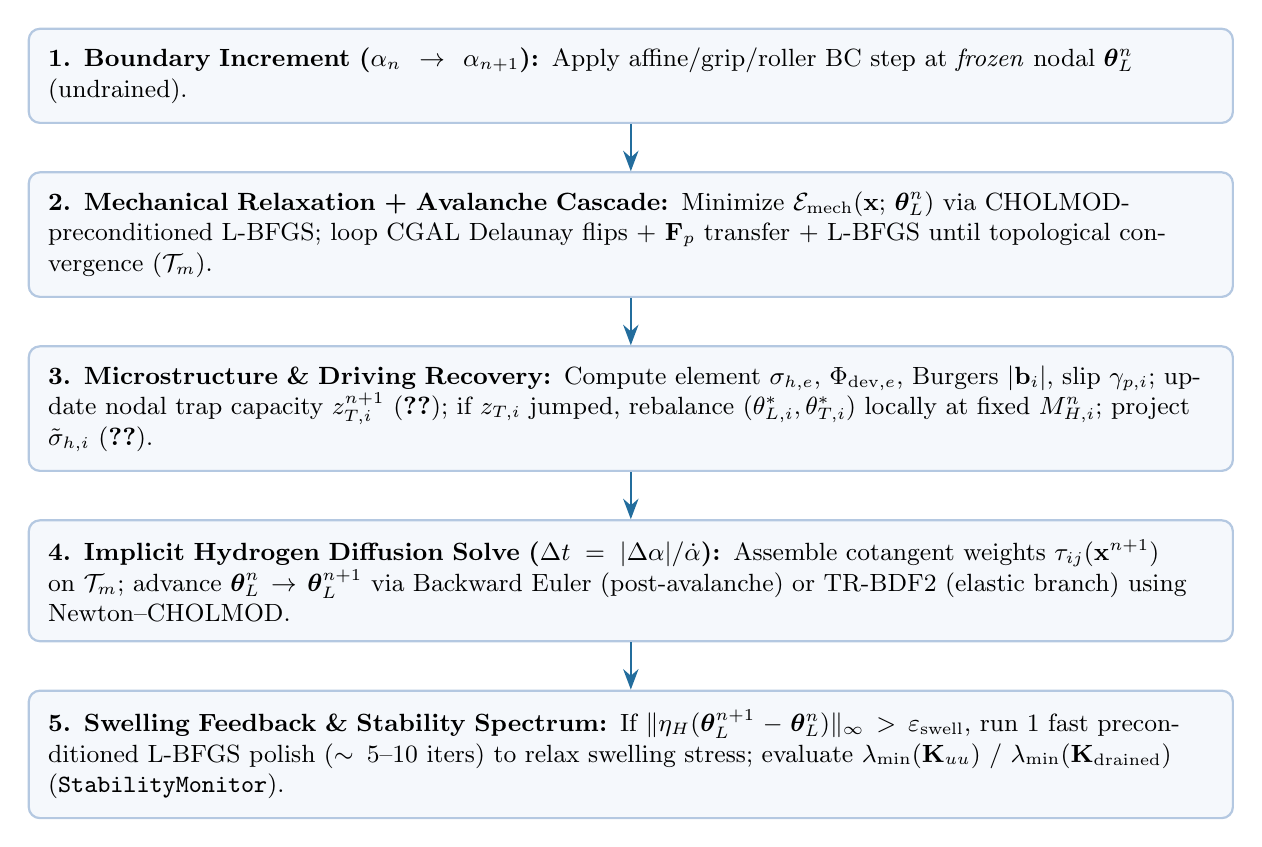
\begin{tikzpicture}[
  node distance=6mm and 10mm,
  stepbox/.style={draw=boxframe,fill=boxbg,rounded corners=4pt,thick,align=left,font=\small,text width=14.8cm,inner sep=7pt},
  arrow/.style={-{Stealth[length=2.6mm]},thick,draw=atomblue!85!black}
]
  \node[stepbox] (s1) {\textbf{1. Boundary Increment ($\alpha_n \to \alpha_{n+1}$):} Apply affine/grip/roller BC step at \emph{frozen} nodal $\boldsymbol{\theta}_L^n$ (undrained).};
  \node[stepbox,below=of s1] (s2) {\textbf{2. Mechanical Relaxation + Avalanche Cascade:} Minimize $\mathcal{E}_{\text{mech}}(\mathbf{x};\,\boldsymbol{\theta}_L^n)$ via CHOLMOD-preconditioned L-BFGS; loop CGAL Delaunay flips + $\mathbf{F}_p$ transfer + L-BFGS until topological convergence ($\mathcal{T}_m$).};
  \node[stepbox,below=of s2] (s3) {\textbf{3. Microstructure \& Driving Recovery:} Compute element $\sigma_{h,e}$, $\Phi_{\text{dev},e}$, Burgers $|\mathbf{b}_i|$, slip $\gamma_{p,i}$; update nodal trap capacity $z_{T,i}^{n+1}$ \eqref{eq:trap_density}; if $z_{T,i}$ jumped, rebalance $(\theta_{L,i}^*, \theta_{T,i}^*)$ locally at fixed $M_{H,i}^n$; project $\tilde{\sigma}_{h,i}$ \eqref{eq:l2_stress_recovery}.};
  \node[stepbox,below=of s3] (s4) {\textbf{4. Implicit Hydrogen Diffusion Solve ($\Delta t = |\Delta\alpha|/\dot{\alpha}$):} Assemble cotangent weights $\tau_{ij}(\mathbf{x}^{n+1})$ on $\mathcal{T}_m$; advance $\boldsymbol{\theta}_L^n \to \boldsymbol{\theta}_L^{n+1}$ via Backward Euler (post-avalanche) or TR-BDF2 (elastic branch) using Newton--CHOLMOD.};
  \node[stepbox,below=of s4] (s5) {\textbf{5. Swelling Feedback \& Stability Spectrum:} If $\|\eta_H(\boldsymbol{\theta}_L^{n+1}-\boldsymbol{\theta}_L^n)\|_\infty > \varepsilon_{\text{swell}}$, run 1 fast preconditioned L-BFGS polish ($\sim 5$--$10$ iters) to relax swelling stress; evaluate $\lambda_{\min}(\mathbf{K}_{uu})$ / $\lambda_{\min}(\mathbf{K}_{\text{drained}})$ (\code{StabilityMonitor}).};

  \draw[arrow] (s1) -- (s2);
  \draw[arrow] (s2) -- (s3);
  \draw[arrow] (s3) -- (s4);
  \draw[arrow] (s4) -- (s5);
\end{tikzpicture}
\caption{Staggered chemo-plastic MTM solution sequence within one load step $\alpha_n \to \alpha_{n+1}$.}
\label{fig:flowchart}
\end{figure}

\noindent
Notice Step~3's local conservation detail: when an avalanche increases $z_{T,i}^n \to z_{T,i}^{n+1}$ by nucleating a new dislocation core, total nodal hydrogen $M_{H,i}^n$ has not yet had time to diffuse in from far away, so solving the scalar quadratic equation $z_L \theta_{L,i}^* + z_{T,i}^{n+1}\theta_T(\theta_{L,i}^*) = M_{H,i}^n$ locally depletes adjacent interstitial sites right before Step~4 draws fresh hydrogen into the core over $\Delta t$!

\subsection{Temporal Integration Order: Why L-Stability Matters Across Avalanches}

Let $A_i = \frac{1}{3}\sum_{e \ni i} A_{0,e}$ be the lumped nodal reference area ($N_L A_i = z_L A_i / \Omega_0$). Semi-discretizing \eqref{eq:h_conservation} gives the stiff nonlinear ODE system
\begin{equation}
  \frac{A_i}{\Omega_0}\frac{d M_{H,i}(\theta_{L,i})}{dt} + \sum_{j \in \mathcal{N}(i)} F_{ij}^{\text{FD}}(\boldsymbol{\theta}_L) = 0,
  \qquad i = 1, \dots, N.
  \label{eq:ode_system}
\end{equation}
Which temporal order should integrate \eqref{eq:ode_system}?
\begin{itemize}[nosep]
  \item \textbf{Never use explicit Euler/RK4:} The diffusive CFL limit $\Delta t_{\text{CFL}} \sim a_0^2 / (4 D_H)$ restricts $\Delta t$ to nanoseconds on an atomic-scale mesh, defeating MTM's ability to reach $\Pi \gtrsim 1$.
  \item \textbf{Avoid pure Crank--Nicolson (trapezoidal 2nd order) across avalanches:} Crank--Nicolson is A-stable ($|R(\infty)| = 1$) but \emph{not} L-stable. Whenever an avalanche occurs in Step~2, $\psi_i$ jumps discontinuously, exciting high-wavenumber modes that oscillate with $(-1)^k$ temporal ringing under Crank--Nicolson.
  \item \textbf{Recommended adaptive temporal order:}
  \begin{enumerate}[nosep]
    \item \textbf{First-order Backward Euler (BDF1, $O(\Delta t)$, L-stable with $R(\infty)=0$)} on any step where an avalanche / Delaunay edge flip occurred (and as the robust default):
    \begin{equation}
      R_i(\boldsymbol{\theta}_L^{n+1}) \;\equiv\;
      \frac{A_i}{\Omega_0}\Bigl[M_{H,i}(\theta_{L,i}^{n+1}) - M_{H,i}^n\Bigr]
      + \Delta t \sum_{j \in \mathcal{N}(i)} F_{ij}^{\text{FD}}(\boldsymbol{\theta}_L^{n+1}) \;=\; 0.
      \label{eq:bdf1_residual}
    \end{equation}
    \item \textbf{Second-order TR-BDF2 ($O(\Delta t^2)$, \emph{also} L-stable with $R(\infty)=0$!)} on smooth elastic branches when higher temporal accuracy is needed at $\Pi \sim 1$: perform one trapezoidal half-step to $t_n + \gamma\Delta t$ ($\gamma = 2 - \sqrt{2}$), followed by a BDF2 step from $(t_n,\, t_n + \gamma\Delta t)$ to $t_{n+1}$. Both stages use the exact same Newton solver structure as \eqref{eq:bdf1_residual}.
  \end{enumerate}
\end{itemize}

\subsection{Quadratic Newton--Raphson Inner Loop with Sparse Factorization}

At each implicit diffusion step, solve $\mathbf{R}(\boldsymbol{\theta}_L) = \mathbf{0}$ in \eqref{eq:bdf1_residual} via damped Newton--Raphson ($\boldsymbol{\theta}_L^{(k+1)} = \boldsymbol{\theta}_L^{(k)} + \omega \Delta\boldsymbol{\theta}_L$, clamping line-search $\omega \in (0,1]$ so $\theta_{L,i}^{(k+1)} \in [10^{-15}, 1 - 10^{-12}]$). From \eqref{eq:ceff} and \eqref{eq:fd_log_mean}, the exact $N \times N$ sparse Jacobian $\mathbf{J} = \partial \mathbf{R} / \partial \boldsymbol{\theta}_L$ has entries
\begin{align}
  J_{ii} &= \frac{A_i}{\Omega_0}\left(z_L + z_{T,i}\frac{d\theta_T}{d\theta_L}\Big|_i\right)
           + \Delta t \sum_{j \in \mathcal{N}(i)} D_H N_L \tau_{ij}
             \left(1 + \frac{\partial M_{ij}^{\text{log}}}{\partial \theta_{L,i}}(\psi_i - \psi_j)\right),
  \label{eq:jac_diag}\\
  J_{ij} &= -\Delta t\, D_H N_L \tau_{ij}
             \left(1 - \frac{\partial M_{ij}^{\text{log}}}{\partial \theta_{L,j}}(\psi_i - \psi_j)\right),
  \qquad j \in \mathcal{N}(i).
  \label{eq:jac_offdiag}
\end{align}
Note a key linear-algebra detail:
\begin{itemize}[nosep]
  \item In the symmetric chemical-potential variable $u_i = \ln\frac{\theta_{L,i}}{1-\theta_{L,i}} + \psi_i$ (or under semi-implicit mobility lagging where $M_{ij}^{\text{log}}$ in the drift term is evaluated at iterate $(k)$, i.e.\ Picard--Newton), the linear system matrix $\tilde{\mathbf{J}}$ is \textbf{strictly Symmetric Positive Definite (SPD)}!
  \item Therefore, your existing \code{SparseCholesky} (CHOLMOD supernodal $LL\T$ in \code{include/\allowbreak{}optimization/\allowbreak{}SparseCholesky.h}) solves each scalar $N \times N$ iteration directly in $< 1\,\mathrm{ms}$ for $N = 40{,}000$ nodes ($199 \times 199$ crystal), converging to $\|\mathbf{R}\|_\infty < 10^{-12}$ in $3\text{--}5$ iterations (or use Eigen's \code{SparseLU} / \code{BiCGSTAB} if retaining the tiny unsymmetric $\partial M_{ij}^{\text{log}}/\partial\theta_L$ term for exact quadratic convergence in $2\text{--}3$ iterations).
\end{itemize}

% ============================================================================
\section{Codebase Integration Map}
\label{sec:code_map}
% ============================================================================

Table~\ref{tab:codebase} summarizes how each mathematical component maps cleanly onto the existing MTM C++ architecture without breaking backward compatibility when hydrogen is disabled ($\theta_L \equiv 0$).

\begin{table}[ht!]
\centering
\small
\renewcommand{\arraystretch}{1.22}
\begin{tabular}{@{}p{4.1cm}p{5.3cm}p{5.8cm}@{}}
\toprule
\textbf{MTM Module / File} & \textbf{Added State / Parameter} & \textbf{Role in Coupled Algorithm} \\
\midrule
\code{Point2D.h} & \code{double theta\_L}, \code{theta\_T}, \code{M\_H} & Conserved nodal H state ($P_1$ DOFs); invariant across Delaunay flips. \\
\code{ElementTriangle2D.h} & \code{double theta\_L\_elem}, \code{theta\_tot\_elem} & Element averages $\frac{1}{3}\sum_{a=1}^3 \theta_{i_a}$; exposes \code{cumulative\_plastic\_slip} $\gamma_p$. \\
\code{EnergyFunctions.h} & Per-element $b_0 = J_H^2(\theta_L)$, $s_{\text{HELP}}$, $K(\theta_{\text{tot}})$ & Evaluates $W_{\text{mech}}$, $\partial W_{\text{mech}}/\partial\mathbf{C}$, and $\partial^2 W_{\text{mech}}/\partial\mathbf{C}^2$ in \eqref{eq:w_mech_coupled}. \\
\code{FEMHessianAssembler.h} & Reads element $(s_{\text{HELP}}, \tilde{K}, J_H^2)$ & Assembles exact $2N\times 2N$ $\mathbf{K}_{uu}$ (and optional $\mathbf{K}_{\text{drained}}$ Schur complement). \\
\code{HydrogenSolver.h/.cpp} \emph{(new)} & $\eta_H$, $D_H$, $\dot{\alpha}$, $T$, $E_B$, $\alpha_{\text{HELP}}$, $\alpha_{\text{HEDE}}$ & Lumped $L^2$ $\tilde{\sigma}_{h,i}$ projection \eqref{eq:l2_stress_recovery}, cotangent $\tau_{ij}$ \eqref{eq:cotangent}, BDF1/TR-BDF2 + CHOLMOD solve. \\
\code{triangulation\_to\_vtk.h} & \code{POINT\_DATA} scalars $\theta_L$, $\theta_T$, $C_{\text{tot}}$, $\tilde{\sigma}_h$ & Visualizes Cottrell atmospheres, GB segregation, and soft-mode quiver arrows in \code{Lattice Launcher}. \\
\bottomrule
\end{tabular}
\caption{Direct mapping of the coupled hydrogen--plasticity formulation into the MTM C++ repository.}
\label{tab:codebase}
\end{table}

\end{document}
